
\chapter{Методы моделирования ондуляторного излучения от пучка с конечным эмиттансом} \label{chapt2}
В представленной работе внимание будет уделено исключительно ондуляторному излучению. Отчасти это мотивировано относительной простотой рассмотрения ондуляторного излучения, по сравнению, например, с вигглерным \cite{geloni_brightness_2014}, с другой ондуляторные источники излучения преимущественно применяются в задачах имиджинга, где дифракционные эффекты играют решающую роль. Тем не менее, формула~\ref{eq:E_bunch}, конечно же, применима как для ондуляторного излучения, так и для вигглерного и излучения из поворотного магнита. 

В случае полностью некогерентного источника для решения задачи моделирования источника излучения подойдёт метод трассировки лучей, а для полностью когерентного источника излучения, т.е. дифракционно ограниченного источника, необходимо использовать подходы волновой оптики. Один из таких подходов реализован в коде SRW  \cite{chubar_accurate_1998}, \cite{chubar_simulation_2006}, где возможно посчитать излучение релятивистского электрона, через произвольную магнитную систему, и далее, полученное излучение, пропагировать через оптическую систему. Также в коде есть возможность расчёта излучения от электронного пучка с конечным эмиттансом, что будет обсуждаться в настоящей Главе. \rr{переписать и сказать про метод сложения амплитуд}.

Альтернативный подход в моделировании частично когерентного излучения основывается на декомпозиции функции взаимной когерентности синхротронного излучения на Гауссовы-Шелл моды (разложение по полиномам Эрмита) описываемый в работах \cite{singer_modelling_2011}, \cite{hua_application_2012}, \cite{khubbutdinov_coherence_2019}, \cite{noauthor_iucr_nodate}. Однако, как отмечают сами авторы в \cite{khubbutdinov_coherence_2019}, \cite{noauthor_iucr_nodate} и аналитически описывается в \cite{geloni_transverse_2008}, разложение по полиномам Эрмита не применимо в случае, когда источник имеет высокую степень когерентности. Так как область когерентности на источнике весьма высока и функции, которые описывают поведение ондуляторного излучения как в дальней зоне, так и на источнике, имеют не гауссову природу.

В текущей главе описывается новый алгоритм моделирования синхротронного излучения, для краткости называемый СЕРВАЛ. Алгоритм основывается на прямом моделировании стохастических процессов при генерации синхротронного излучения, вызванных дробовым шумом в электронном пучке, с последующим ограничением пространственных гармоник шума огибающими излучения. По своей природе алгоритм имеет оценочный характер, именно поэтому в главе приведён сравнительный анализ результатов СЕРВАЛа с методом сложения амплитуд\footnote{Для определённости, в текущей главе также будет дано принципиальное описание МСА}, на примере некоторых оптических систем. СЕРВАЛ показал себя как мощный инструмент для оценки когерентных свойств синхротронного излучения, с точностью мало уступающей методу сложения амплитуд, а главное имеющий преимущество в быстродействии. 
\section{Численное моделирование ондуляторного излучения}
%\begin{align}
%\widetilde{E}_{\bot}(0, \vec{r}_{\bot}) =
%i \frac{e A_{JJ} \omega}{2 c^2}\frac{K}{\gamma} \times \bigg [\pi - 2\text{Si} \bigg( \cfrac{i \omega \vec{r}_{\bot}^{2}}{L_w c}\bigg)\bigg].
%\label{eq:single_electron_near_field_z=0}
%\end{align}

Формула~\ref{eq:E_bunch} используется напрямую при моделирования ондуляторного излучения, как продольно когерентного так и некогерентного. Общий вид поля ондуляторного излучения от одного электрона с некоторыми углом $\vec{\eta}_k$ и координатой $\vec{\l}_k$ может быть записан как \cite{geloni_fourier_2007} \rr{спросить Джанлуку про эту формулу}: 
\begin{align}
	\bar{E}_{\bot}(z_0, \omega, \vec{\eta}_k, \vec{l}_k, \vec{\theta} \;) =
&	-\frac{\omega e A_{JJ} L_s}{2c^2z_0}\frac{K}{\gamma}\exp{\bigg[i \frac{\omega z_0}{2c} \bigg|\vec{\theta} - \vec{\l}/z_0\bigg|^2 \bigg]} \cr & \times \sinc \bigg[\bigg(k_w \frac{\Delta \omega}{\omega} + \frac{\omega |\vec{\theta} - (\vec{\l}/z_0) - \vec{\eta}|^2}{2c}\bigg)\cfrac{L_s}{2}\bigg],
	\label{eq:single_electron_far_field}
\end{align}
где $\vec{\theta} = \vec{r}/z_0$ \rr{пояснить все новые параметры}. Формула \ref{eq:single_electron_far_field} даёт распределение амплитуды поля в дальней зоне ($z_0 \gg L_w$\rr{и что-то ещё}). Чтобы получить более точно выражение это поле должно быть отпропагировано назад в центр ондулятора с помощью пропагатора свободного пространства. Распределение поля в мнимом источнике излучения: \rr{Откуда взялась информация, которой не было. Нужна пояснительная команда.}
\begin{align}
	\widetilde{E}_{\bot}(0, \vec{\eta}, \vec{\l}, \vec{r}_{\bot}) =
	i \frac{e A_{JJ} \omega}{2 c^2}\frac{K}{\gamma} &\exp{\big[i \frac{\omega}{c} (\vec{r}_{\bot} - \vec{l})\big]}\cr & \times \bigg [\pi - 2\text{Si} \bigg( \cfrac{i \omega |\vec{r}_{\bot} - \vec{l}|^2}{L_w c}\bigg)\bigg], 
	\label{eq:single_electron_near_field_z=0}
\end{align}
после этого поле можно распространять на любую дистанцию вдоль оптической оси $z_0$. Снова применяя пропагатор свободно пространства, получаем:
\begin{align}
	\bar{E}_{\bot}(&z_0, \omega, \vec{\eta}_k, \vec{\l}_k, \vec{r}) =
		\frac{e A_{JJ} \omega}{2 c^2}\frac{K}{\gamma} \exp{\bigg[i \frac{\omega}{2 z_0 c} (|\vec{r}_{\bot} - \vec{l}|^2 - |\vec{r}_{\bot} - \vec{l} - z_0 \vec{\eta}|^2) \bigg]} \cr & \times	\bigg \{ \text{Ei} \bigg[ \cfrac{i \omega (\vec{r}_{\bot} - \vec{l} - z_0 \vec{\eta})^2}{2z_0c - L_w c}\bigg] - \text{Ei} \bigg[ \cfrac{i \omega (\vec{r}_{\bot} - \vec{l} - z_0 \vec{\eta})^2}{2z_0c + L_w c} \bigg] \bigg\}.
	\label{eq:single_electron_near_field}
\end{align}
Рассчитанное таким образом поле может быть рассчитано для любого значения $z_0$, такое поле называют поле в приближении ближней зоны, так как эта формула применим для значение $z_0 \sim L_w$. Обе формулы \ref{eq:single_electron_far_field} и \ref{eq:single_electron_near_field} имеют практическую ценность при моделировании, однако при использовании выражения \ref{eq:single_electron_near_field} время на моделирование значительно увеличивается, так как необходимо дважды численно взять интеграл $\textup{Ei}(\cdot)$.
 
После расчёта суммарного поля c $N_e$ электронами получившиеся монохроматическое поле по своей сути есть одна статистическая реализация поля. \rr{переформулировать следующее предложение} Физически это значит следующее, если экспериментатор измерит распределение интенсивности поля на детекторе от пролёта одного электронного пучка, используя монохроматор с разрешением, которое позволит разрешить одну продольную моду излучения, то на детекторе будет распределение эквивалентное по своим статистическим свойствам распределению, представленному на Рис.. 

После усреднения по $N_b$ реализациям (с идеальным монохроматором\footnote{другими словами, монохроматором разрешается одна поперечная мода}), наблюдаемая интенсивность даётся выражением: 
\begin{align}
	I_{\omega} = \bigg \langle \bigg|\sum\limits_{k=1}^{N_e} \bar{E}(\vec{\eta}_k, \vec{\l}_k, z, \vec{r}, \omega) \exp{(i \omega t_k)}\bigg|^2 \bigg \rangle,
	\label{eq:I_MC} 
\end{align}
\begin{figure}[H] 
	\centering 	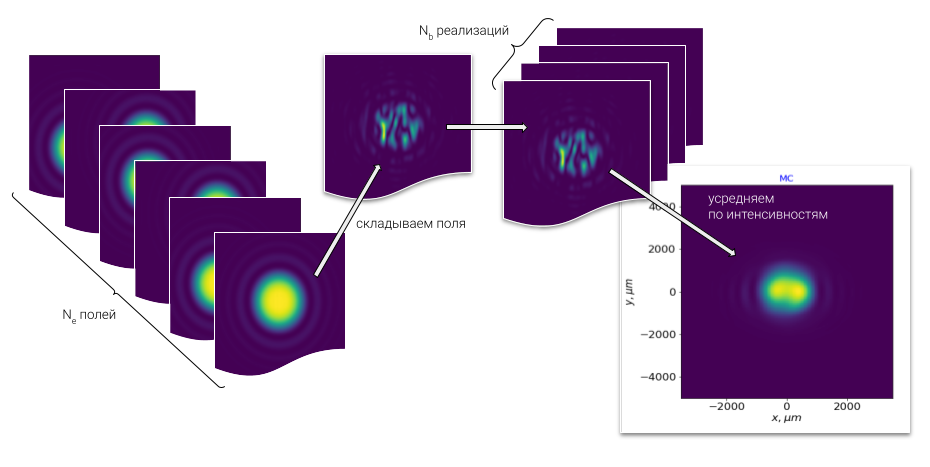
\includegraphics[width=0.99\linewidth]{MC_scheme.png}
	\caption{Схема работы метода сложения амплитуд}
	\label{fig:SRW_scheme}
\end{figure}
\rr{сделать заметку, что чем хуже когерентности тем больше реализаций нужно, чтобы получить гладкое решение}
\noindent результирующая интенсивность будет сходиться к некоторой огибающей. В грубом приближении огибающая является свёрткой распределения расходимости излучения и распределения расходимости электронного пучка. Данный подход является наиболее прямым подходом к задаче моделирования частично когерентного излучения, однако время расчёта в таком случае может быть оценено как время затрачиваемое на расчёт одной одного поля $N_e$ раз по формуле~\ref{eq:single_electron_far_field} или~\ref{eq:single_electron_near_field}, в последней, как уже упоминалось, необходимо дважды численно взять интеграл $\textup{Ei}(\cdot)$ и потом усреднить по $N_b$ реализациям поля $\bar{E}_{b}$. Итого, если за $\tau_{calc}$ взять время расчёта одного поля, то расчёт одного результирующего поля в сумме займёт $T_{calc} = \tau_{calc} \cdot N_e \cdot N_b$.

Однако в случае полностью некогерентного излучения время расчёта можно сократить за счёт фазового фактора $\exp{(i \omega t_k)}$, который эффективно приводит к тому, что отдельный электрон в электронном пучке коррелирует только с самим собой \cite{geloni_transverse_2008}. Таким образом формула~\ref{eq:I_MC} упрощается до 
\begin{align}
 	I_{\omega} = \sum\limits_{k=1}^{N_e} \bigg|\bar{E}(\vec{\eta}_k, \vec{\l}_k, z, \vec{r}, \omega)\bigg|^2,
 	\label{eq:I_SRW} 
\end{align}
\begin{figure}[H] 
	\centering 	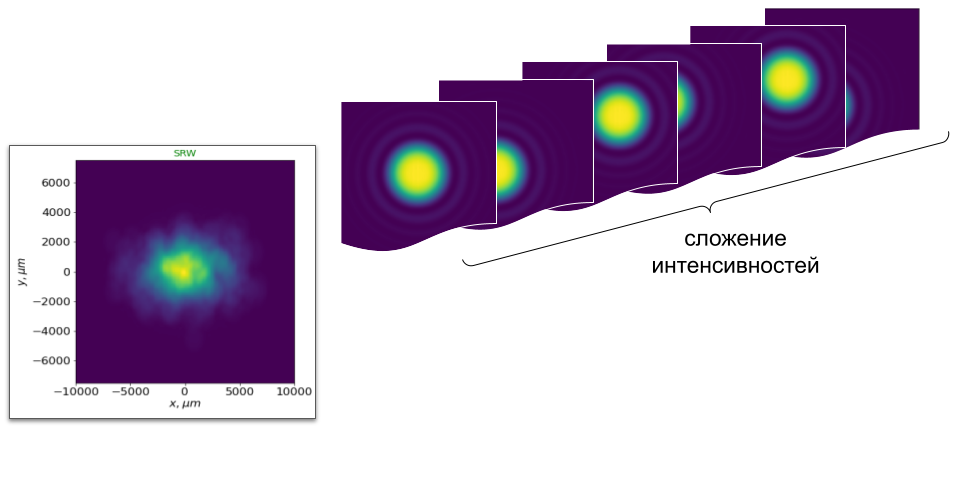
\includegraphics[width=0.99\linewidth]{SRW_scheme.png}
	\caption{Схема метода сложения интенсивностей}
	\label{fig:SRW_scheme}
\end{figure}
\noindent а время расчёта уменьшается до $T_{calc} = \tau_{calc} \cdot N_e$. Недостатком такого подхода можно считать потерю фазовой информации о излучение и, следовательно, невозможности расчёта поперечной автокрелляционной функции первого порядка \rr{Можно ли через второй порядок найти первый? Нужна пояснительная команда}. Тем не менее, подход основанный на формуле~\ref{eq:I_SRW} даёт мощный метод расчёта частично когерентного излучения. Именно этот подход реализован в широко распространённом коде SRW \rr{cite}.
 
\subsection{Влияние размера электронного пучка на расходимость излучения}
\rr{где такой эффект можно неожиданно встретить?}

\rr{продольно когерентный случай, CSR}
\begin{figure}[H] 
	\centering 	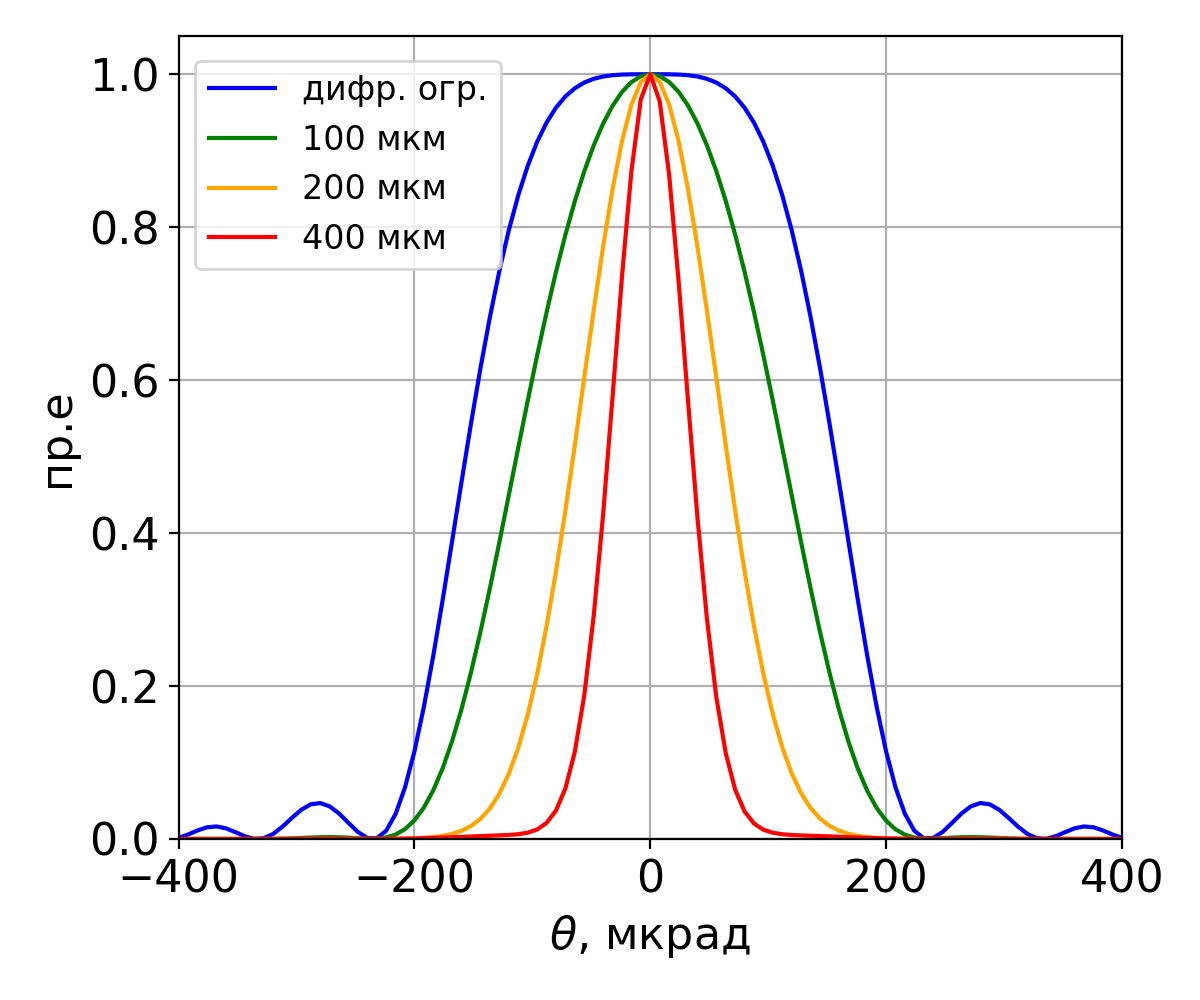
\includegraphics[width=0.99\linewidth]{diff_divergence_coh.png}
	\caption{\rr{Подпись, изменить цвет линий на синий зелёный, легенда}}
	\label{fig:diff_coh_incoh_rad}
\end{figure}

\rr{некогерентный случай, варианты с различной бета-функцией}
\begin{figure}[H] 
	\centering 	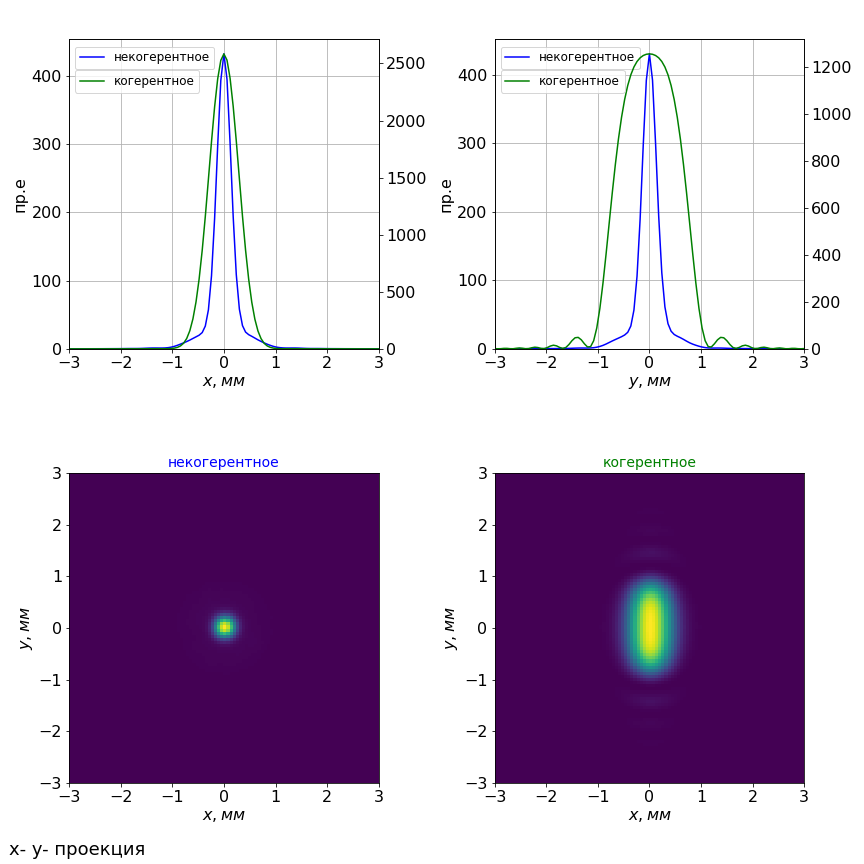
\includegraphics[width=0.99\linewidth]{diff_divergence_incoh.png}
	\caption{\rr{Подпись, изменить цвет линий на синий зелёный, легенда}}
	\label{fig:diff_coh_incoh_rad}
\end{figure}

\subsection{Различие расходимости излучения для случая продольно полностью когерентного и некогерентного пучка}
В зависимости от длительности электронного пучка результирующее поле $\bar{E}_{b}$ будет вести себя по-разному. В случае короткого электронного пучка: $\omega \sigma_T \ll 1$, где $\sigma_T$ -- длительность электронного сгустка, излучение будет продольно когерентным, в иностранной литературе этот эффект называется Coherent Synchrotron Radiation (CSR). Методы моделирования такого излучения рассмотрены в работах \rr{cite}. Приближение короткого электронного пучка справедливо для низких энергий \rr{каких?}. Случай длинного электронного пучка, а именно  $\omega \sigma_T \gg 1$ соответствует случаю продольно некогерентного излучения, а для уравнения~\ref{eq:E_bunch} это означает, что показатель экспоненты $\omega \sigma_T$ равномерно распределён в интервале от $0$ до $2 \pi$. 

\rr{отличие на $\sqrt{2}$}

\rr{где такой эффект можно неожиданно встретить? Вероятнее всего на XFEL, в случае когда пучок обычный (16 фс) и скомпрессированный пучок}
\begin{figure}[H] 
	\centering 	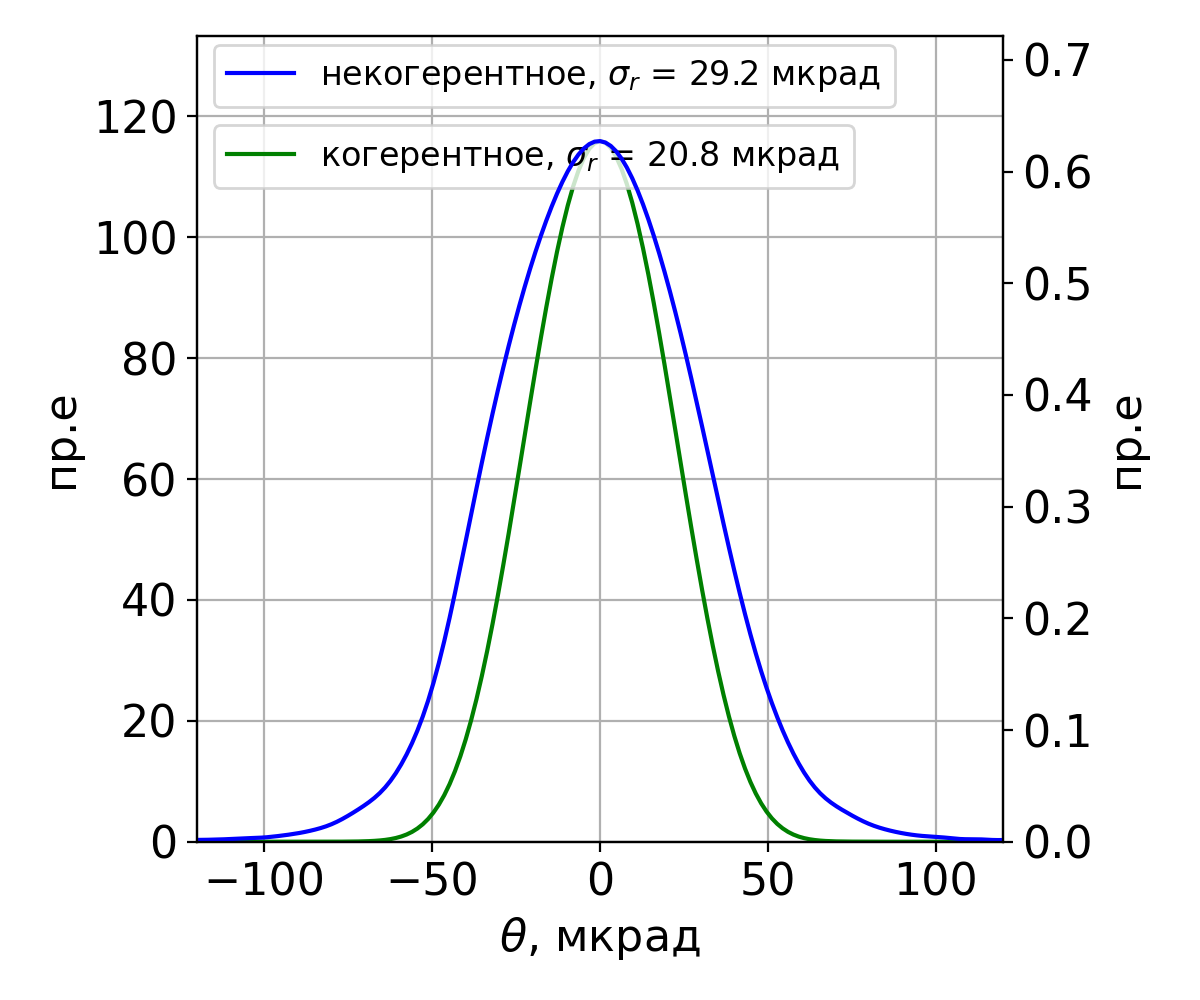
\includegraphics[width=0.99\linewidth]{diff_coh_incoh_rad.png}
	\caption{Интенсивность комплексного гауссового шума \rr{перерисовать в чб}}
	\label{fig:diff_coh_incoh_rad}
\end{figure}
\section{Метод ограничения пространственных гармоник огибающими: СЕРВАЛ}
Предлагаемый метод основывается на моделировании стохастического характера ондуляторного синхротронного излучения комплексным гауссовым шумом с последующим его ограничением огибающими поля. Для начала алгоритм будет представлен в общем виде, без уточнения чем определяются распределение огибающих, задающих размер и расходимость излучения и, в целом, безотносительно характера ондуляторного источника излучение. 
\subsection{Алгоритм создания поля}
Алгоритм создания поля представлен ниже: 
\begin{enumerate}
\item \label{noise} Создание комлексного гауссового шума $Z = X + iY$ в $r\omega$-пространстве, где величины $X$ и $Y$ подчиняются нормальному распределению.
\begin{figure}[H] 
	\centering 	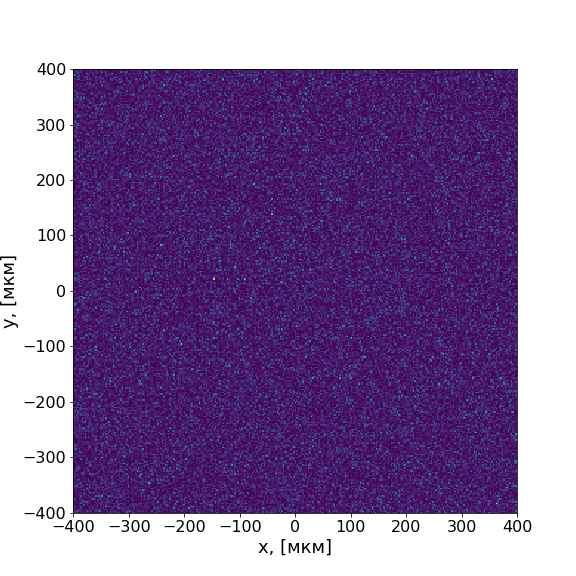
\includegraphics[width=0.45\linewidth]{1-X_noise.png}
	\caption{Интенсивность комплексного гауссового шума}
	\label{fig:1-noise}
\end{figure}
\item \label{beam_s} Ограничение шума эффективным размером электромагнитного излучения в источнике излучения в \textit{r$\omega$}-пространство.
\begin{figure}[H]
	\centering
	\begin{minipage}{0.45\textwidth}
		\centering
		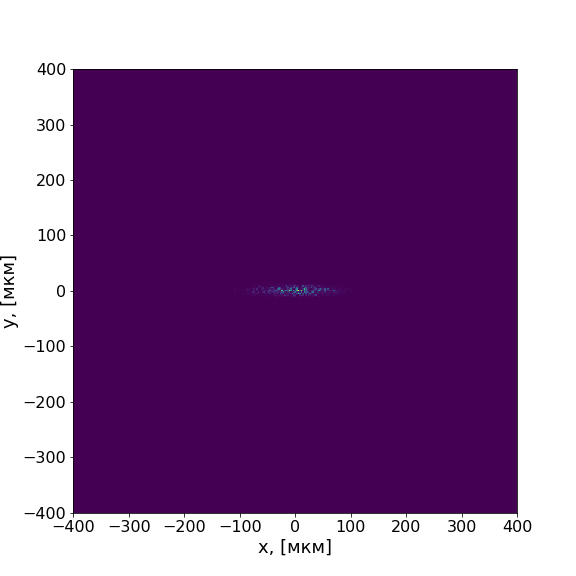
\includegraphics[width=1\linewidth]{2-X_e-beam-size.png}
		\caption{Размер электромагнитного излучения в перетяжке наложенный на шум}
		\label{fig:2-beam_size_k}
	\end{minipage}
	\begin{minipage}{0.45\textwidth}
		\centering
		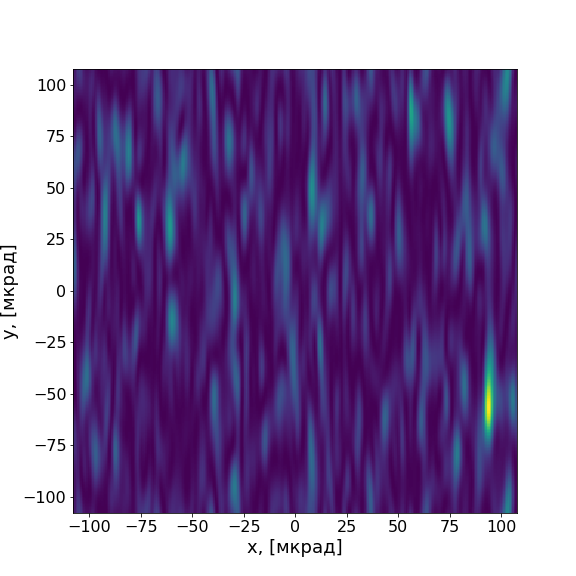
\includegraphics[width=1\linewidth]{2-X_e-beam-divergence.png}
		\caption{Получившиеся моды в $k\omega$-пространстве от размера электронного пучка}
		\label{fig:2-beam_size_s}
	\end{minipage}\hfill
\end{figure}
\item \label{beam_k} Ограничение пространственных мод эффективной расходимостью излучения в \textit{k$\omega$}-пространстве
\begin{figure}[H]
	\centering
	\begin{minipage}{0.45\textwidth}
		\centering
		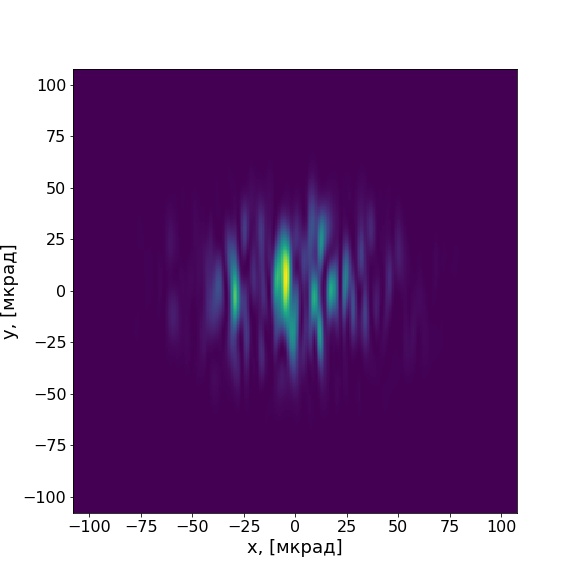
\includegraphics[width=1\linewidth]{3-X_radaition_divergence.png}
		\caption{Расходимость излучения в источнике}
		\label{fig:3-beam_s}
	\end{minipage}
	\begin{minipage}{0.45\textwidth}
		\centering
		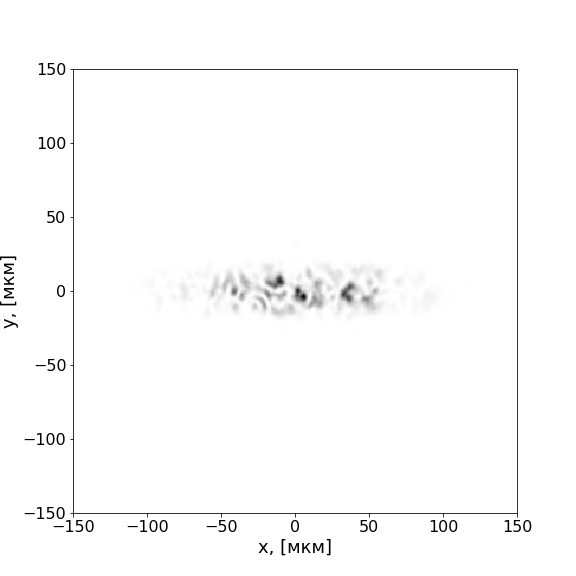
\includegraphics[width=1\linewidth]{3-X_radaition_size.png}
		\caption{Размер излучения в источнике}
		\label{fig:3-beam_k}
	\end{minipage}
\end{figure}
\item Получившиеся распространение поля есть распределение поля в источнике излучения (центр ондулятора).
\end{enumerate}
Быстродействие алгоритма можно оценить следующим образом: алгоритм генерирует $N_x \cdot N_y \cdot N_b$ случайный величин подчиняющихся распределению $Z$, где $N_b$ -- количество реализаций поля, одно Фурье преобразование поля (преобразование поля на Рис.~\ref{fig:2-beam_size_k} в поле на Рис.~\ref{fig:2-beam_size_s}) и две операции умножения на огибающие поля. Получившиеся поле, представленное на Рис.~\ref{fig:3-beam_k}, уже готово к пропагации, так как пропагатор через свободное пространство работает именно в $kf$-пространстве.
\subsection{Выбор подходящих огибающих}
До этого момента, в работе не обсуждался выбор подходящих огибающих для поля. Вопрос выбора таких огибающих сводится нахождению распределения поля в центре ондулятора. Поле в центре может быть получено, обратной пропагацией излучения из дальней зоны обратно в центр ондулятора при помощи пропагатора излучения в свободном пространстве \rr{cite}. Однако, нахождение аналитического решения уравнения Максвелла в дальней зоне от целого электронного пучка -- не тривиальная задача.  Для оценки можно предположить, что распределение поля ондуляторного излучения от электронного пучка с конечным эмиттансам, в целом, может быть представлено как свёртка распределения поля ондуляторного излучения от одного электрона с распределением фазового пространства электронного пучка.

Для SERVAL можно предложить, как минимум, три вида огибающих для пространственного распределения источника в $r$-пространстве:
\begin{enumerate}[label=\Roman*.]
	\item \label{amplitude} ${A}_{b} (\vec{r}_{\bot}) = \big(\widetilde{E}_{\bot}(0, \vec{l}, \vec{\eta}, \vec{r}_{\bot}) \ast f_l(\vec{l})\big)(\vec{l})$ \\

	\item \label{intensity} ${A}_{b} (\vec{r}_{\bot}) = \sqrt{\big(\widetilde{E}^2_{\bot}(0,  \vec{l}, \vec{\eta}, \vec{r}_{\bot}) \ast f_l^2(\vec{l})\big)(\vec{l})}$ \\

	\item \label{e-beam} ${A}_{b} (\vec{r}_{\bot}) = f_l(\vec{l})$,
\end{enumerate}
и три вида огибающих для распределения расходимости источника ($k$-пространство):
\begin{enumerate}[label=\Roman*.]
	\item \label{amplitude} $\hat{{A}}_{b} (\vec{\theta}_{\bot}) = \big(\hat{\widetilde{E}}_{\bot}(0,  \vec{l}, \vec{\eta}, \vec{\theta}_{\bot}) \ast \hat{f}_{\eta}(\vec{\eta})\big)(\vec{\eta})$\\
	
	\item \label{intensity} $\hat{{A}}_{b} (\vec{\theta}_{\bot}) = \sqrt{\big(\hat{\widetilde{E}^2}_{\bot}(0,  \vec{l}, \vec{\eta}, \vec{\theta}_{\bot}) \ast \hat{f_{\eta}^2}(\vec{\eta})\big)(\vec{\eta})}$\\
	
	\item \label{e-beam} $\hat{{A}}_{b} (\vec{\theta}_{\bot}) = \hat{f}_{\eta}(\vec{\eta})$,
\end{enumerate}
где ${A}_{b} (\vec{r})$ и $\hat{{A}}_{b} (\vec{\theta})$ огибающие в $r$- и $k$-пространствах соответствующие шагам~\ref{beam_s} и~\ref{beam_k} в алгоритме,  $f(\vec{l}, \vec{\eta}) = f_l(\vec{l}) f_{\eta}(\vec{\eta})$ фазовое распределение электронного пучка, и поле $\widetilde{E}_{\bot}(z=0, \vec{\l}, \vec{\eta}, \vec{r}_{\bot})$, $\hat{\widetilde{E}}_{\bot}(z=0 , \vec{\l}, \vec{\eta}, \vec{\theta}_{\bot})$ -- распределение поля взятого в центре ондулятора по формулам \ref{eq:single_electron_far_field}(или более точно \ref{eq:single_electron_near_field}) и \ref{eq:single_electron_near_field_z=0}.

Для выбора подходящих амплитуд было проведено моделирование с различными огибающими в сравнение с эталонным в этой работе методом сложения амплитуд. Для начала необходимо проверить распределение интенсивности поля на источнике. Для метода сложения амплитуд поле было рассчитано в дальней зоне и отпропагировано назад в центр ондулятора. Результаты сравнения приведены на Рис.~\ref{fig:SERVAL_envelopes_comparison_far_zone} при параметрах электронного пучка \rr{параметры электронного пучка}
\begin{figure}[H] 
	\centering 	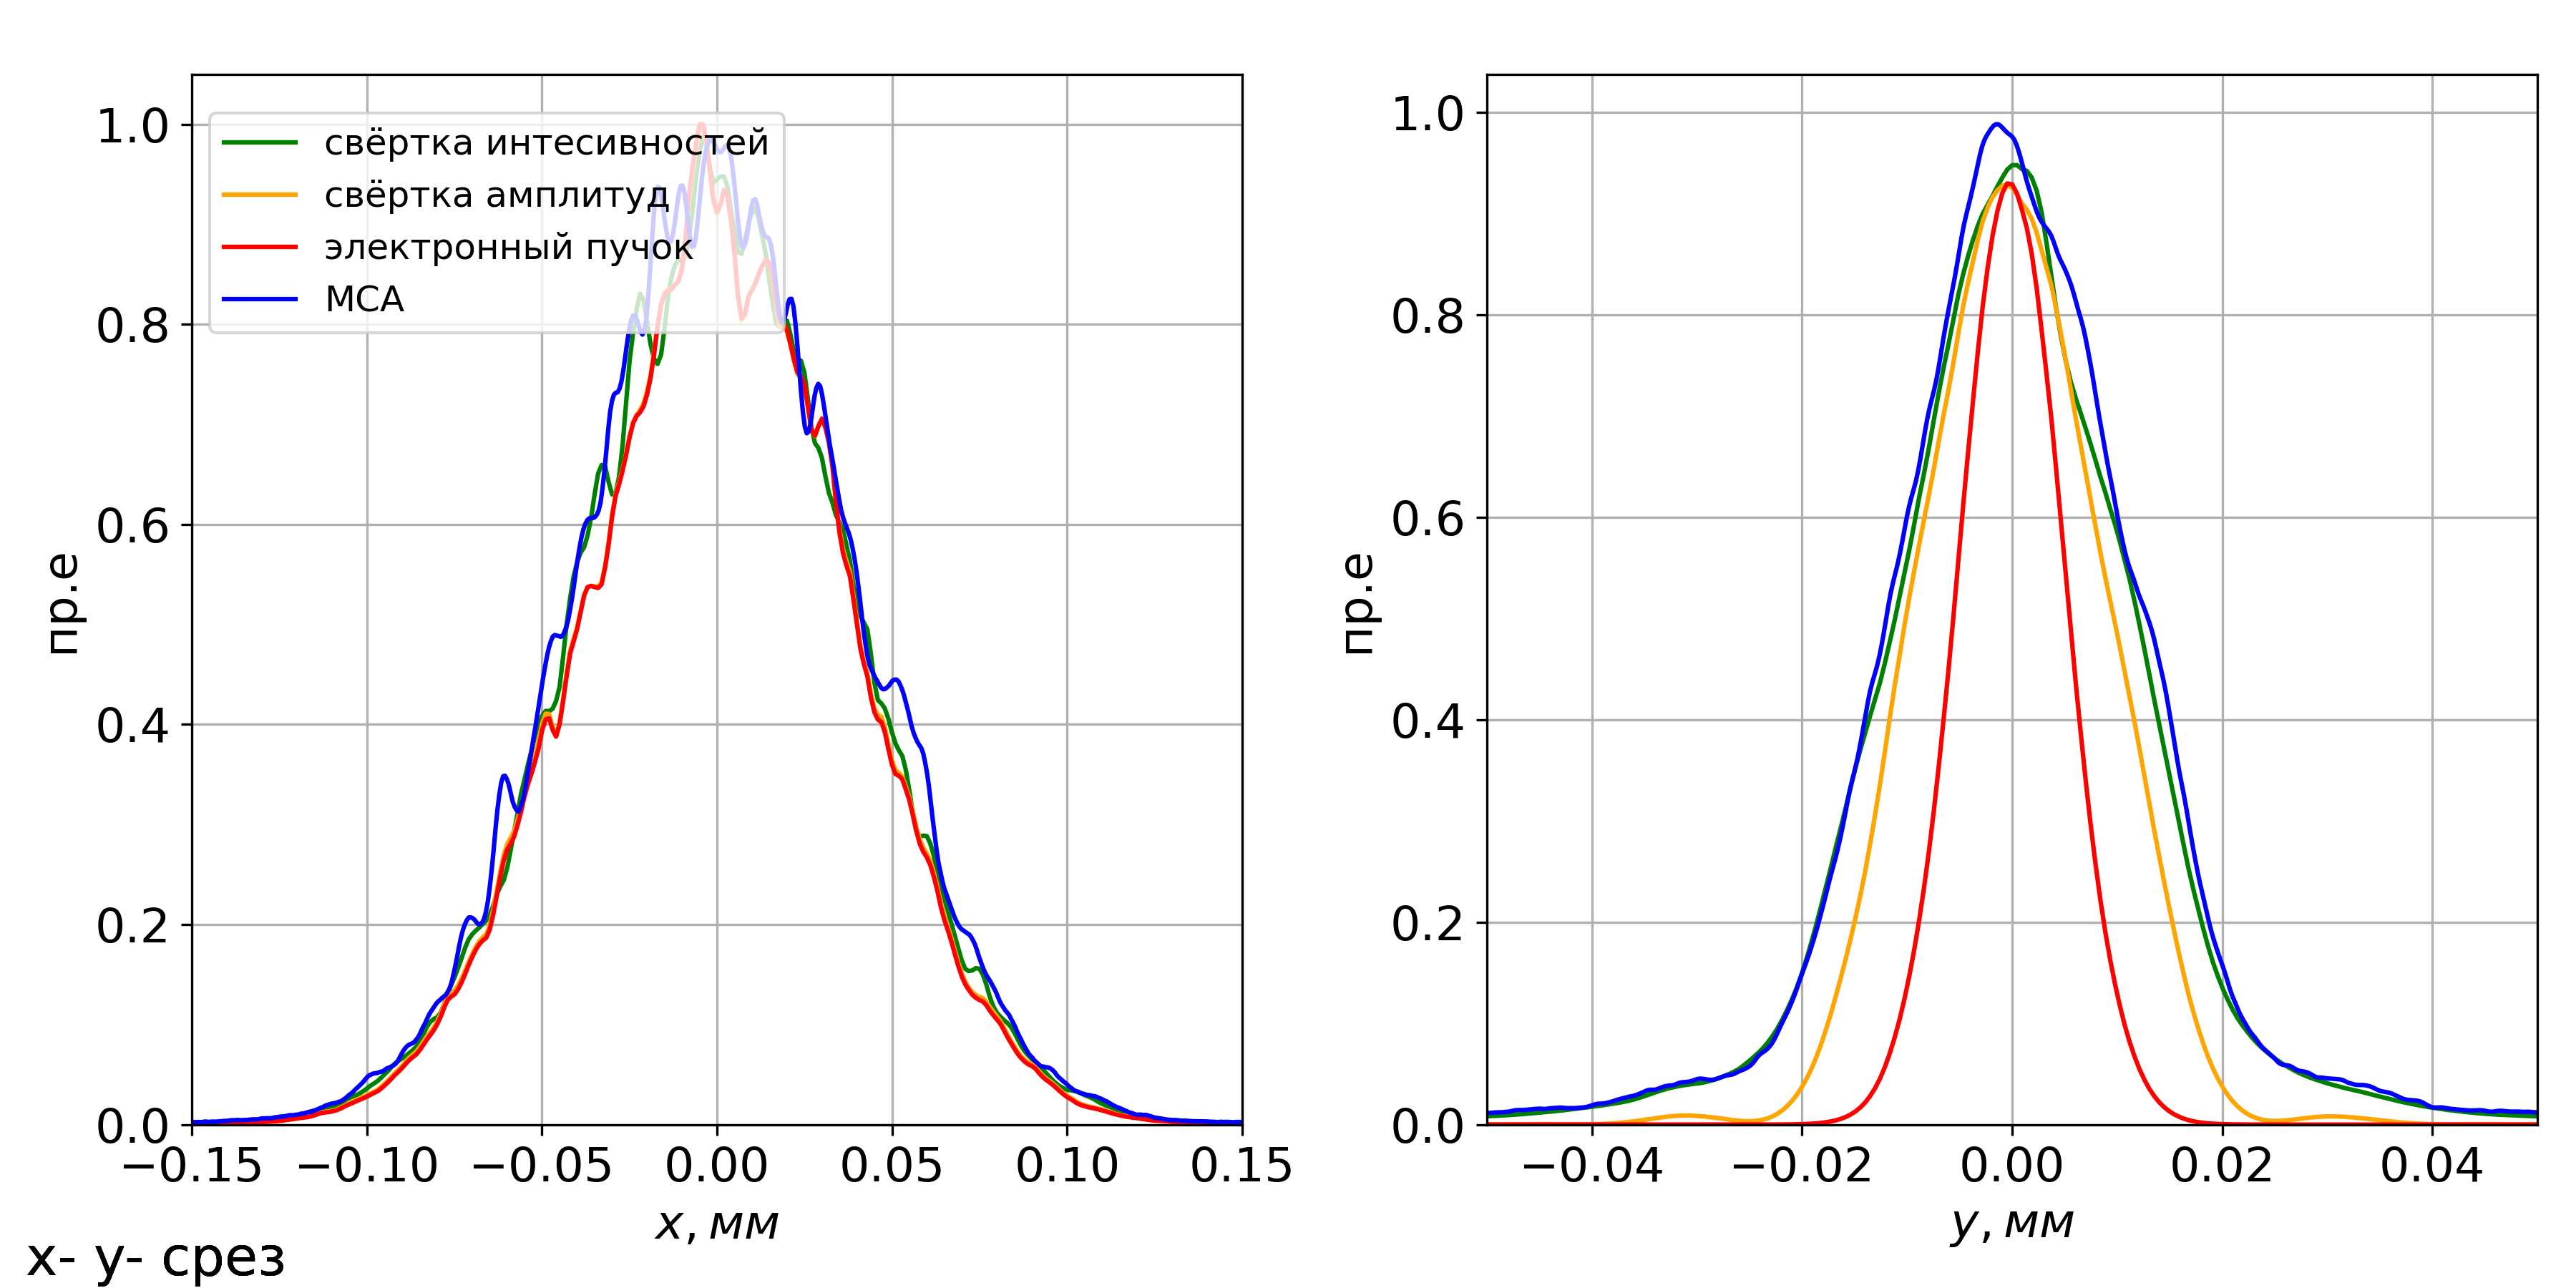
\includegraphics[width=0.99\linewidth]{SERVAL_envelopes_comparison_source.png}
	\caption{Распределение поля в источнике излучения}
	\label{fig:SERVAL_envelopes_comparison_far_zone}
\end{figure}
Видно, что оптимальные результаты достигаются при использовании свёртки~\ref{intensity}. Однако, если $N \ll 1$ или даже просто $N > 1$, то можно использовать любые из представленных огибающих для $r$-пространства. Необходимо так же сравнить корреляционные функции получившихся полей~\ref{fig:diff_coh_incoh_rad}, используя формулу~\ref{eq:g1}.
\begin{figure}[H] 
	\centering 	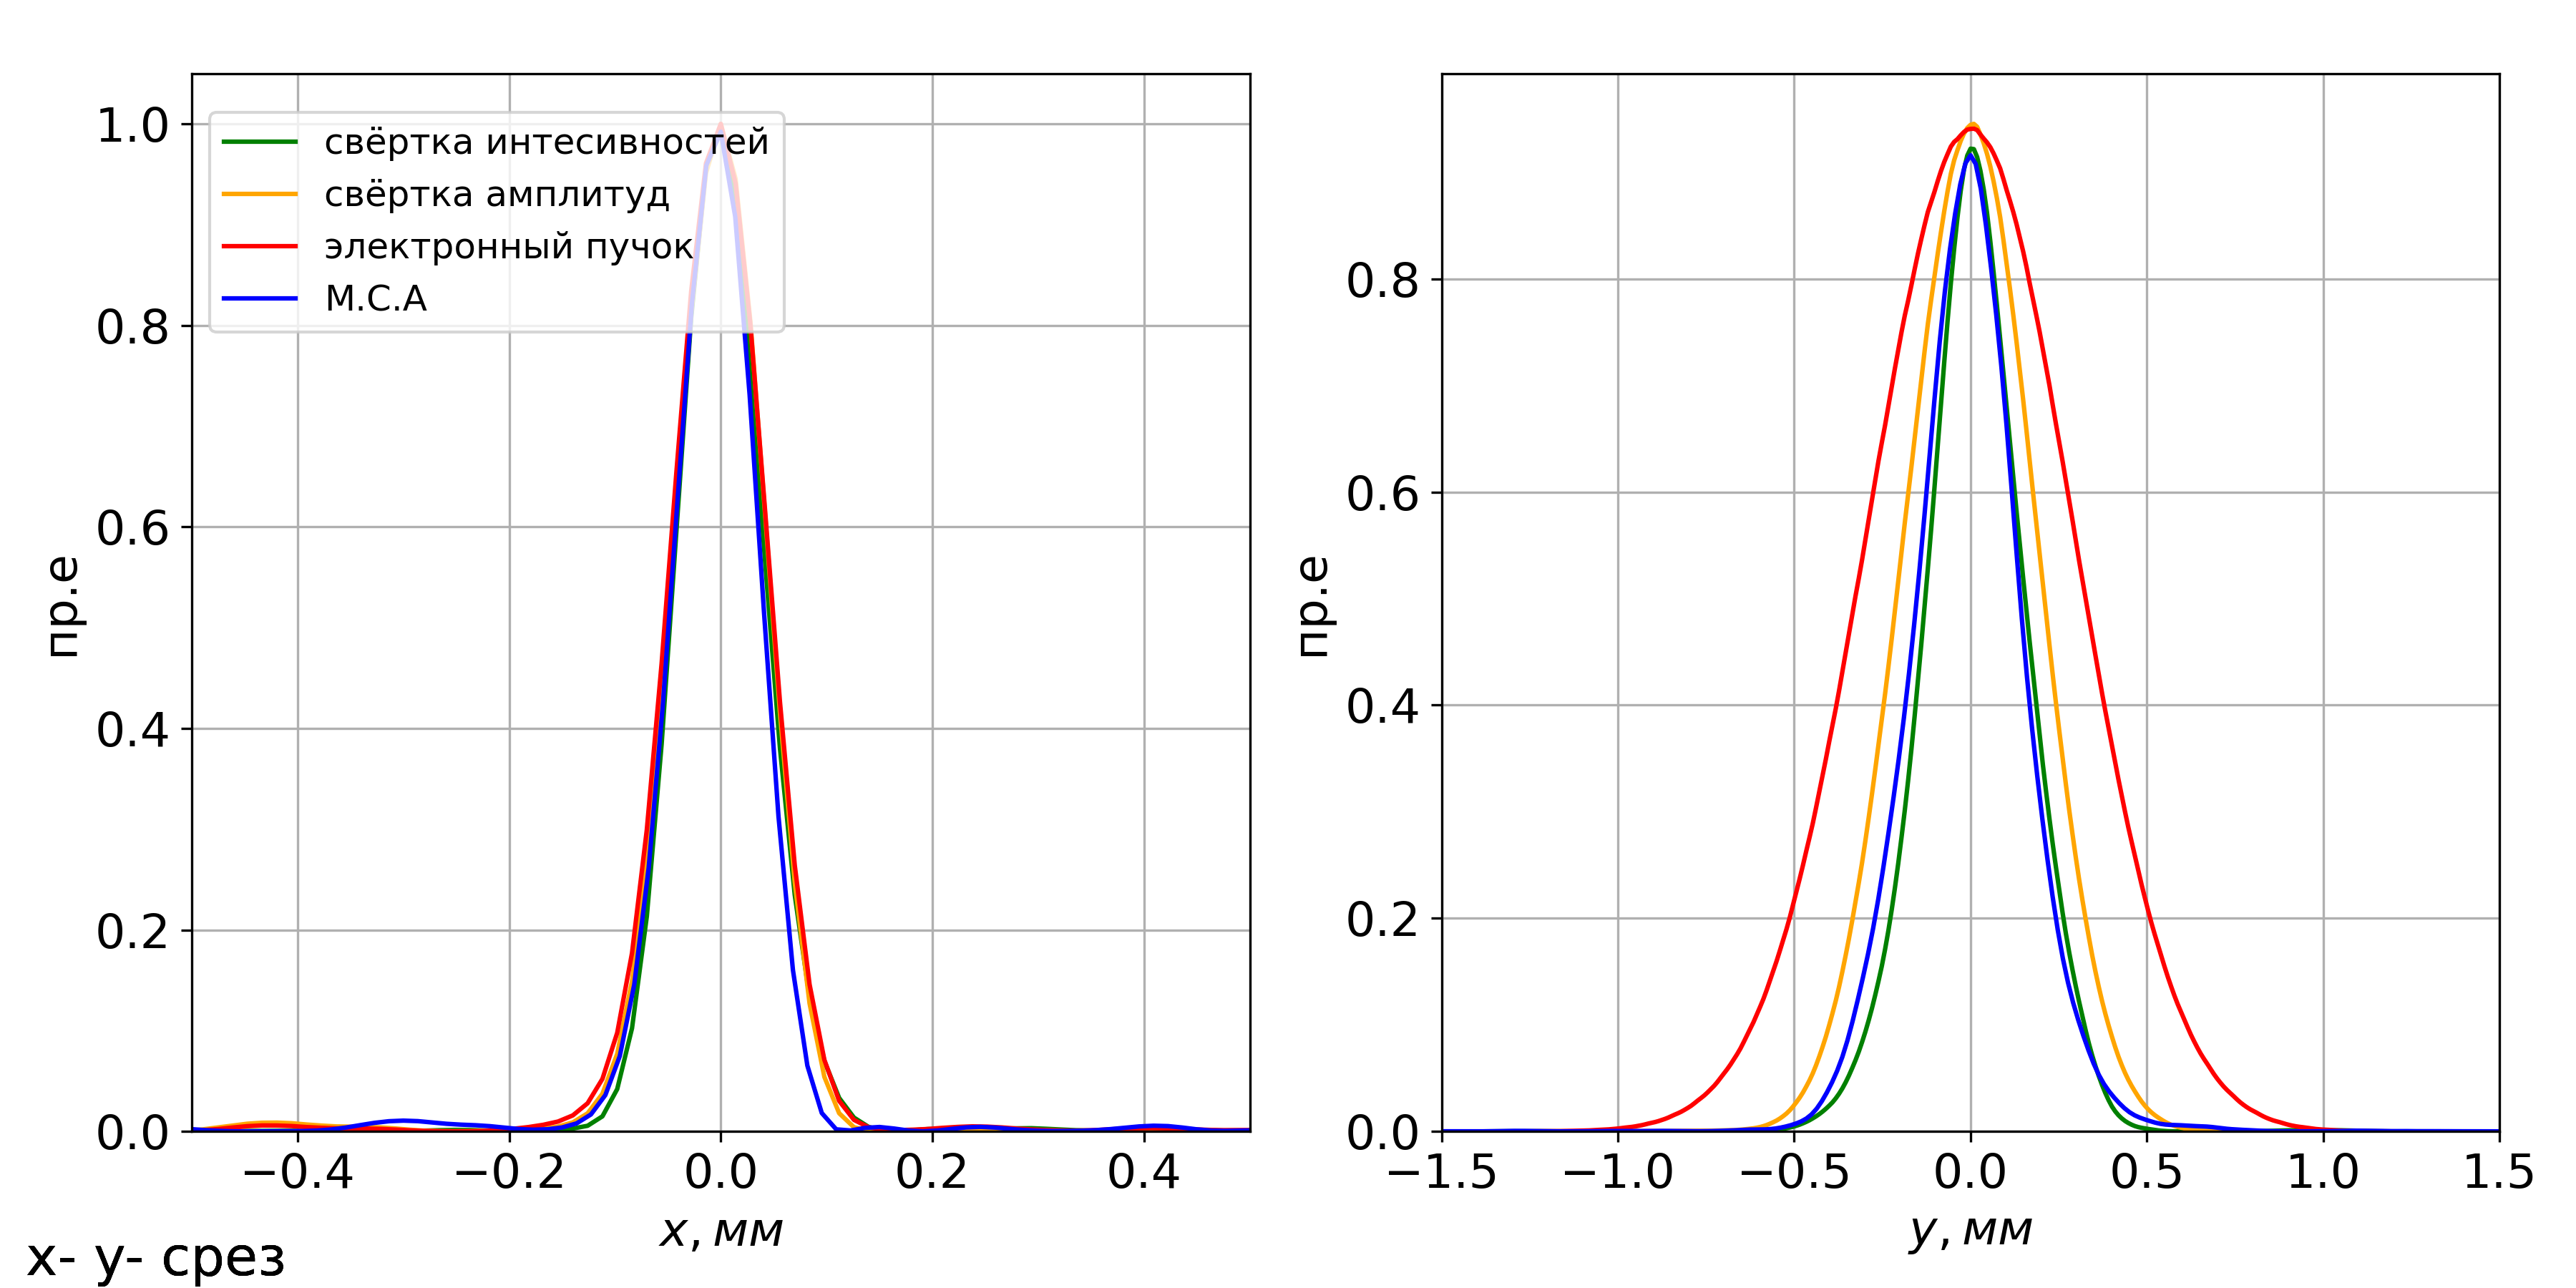
\includegraphics[width=0.99\linewidth]{SERVAL_corr_comparison.png}
	\caption{Функция взаимной когерентности на расстоянии $25$ м от источника}
	\label{fig:SERVAL_corr_comparison}
\end{figure}
Для распределения расходимости следует так же использовать использовать свёртку интенсивностей.
\begin{figure}[H] 
	\centering 	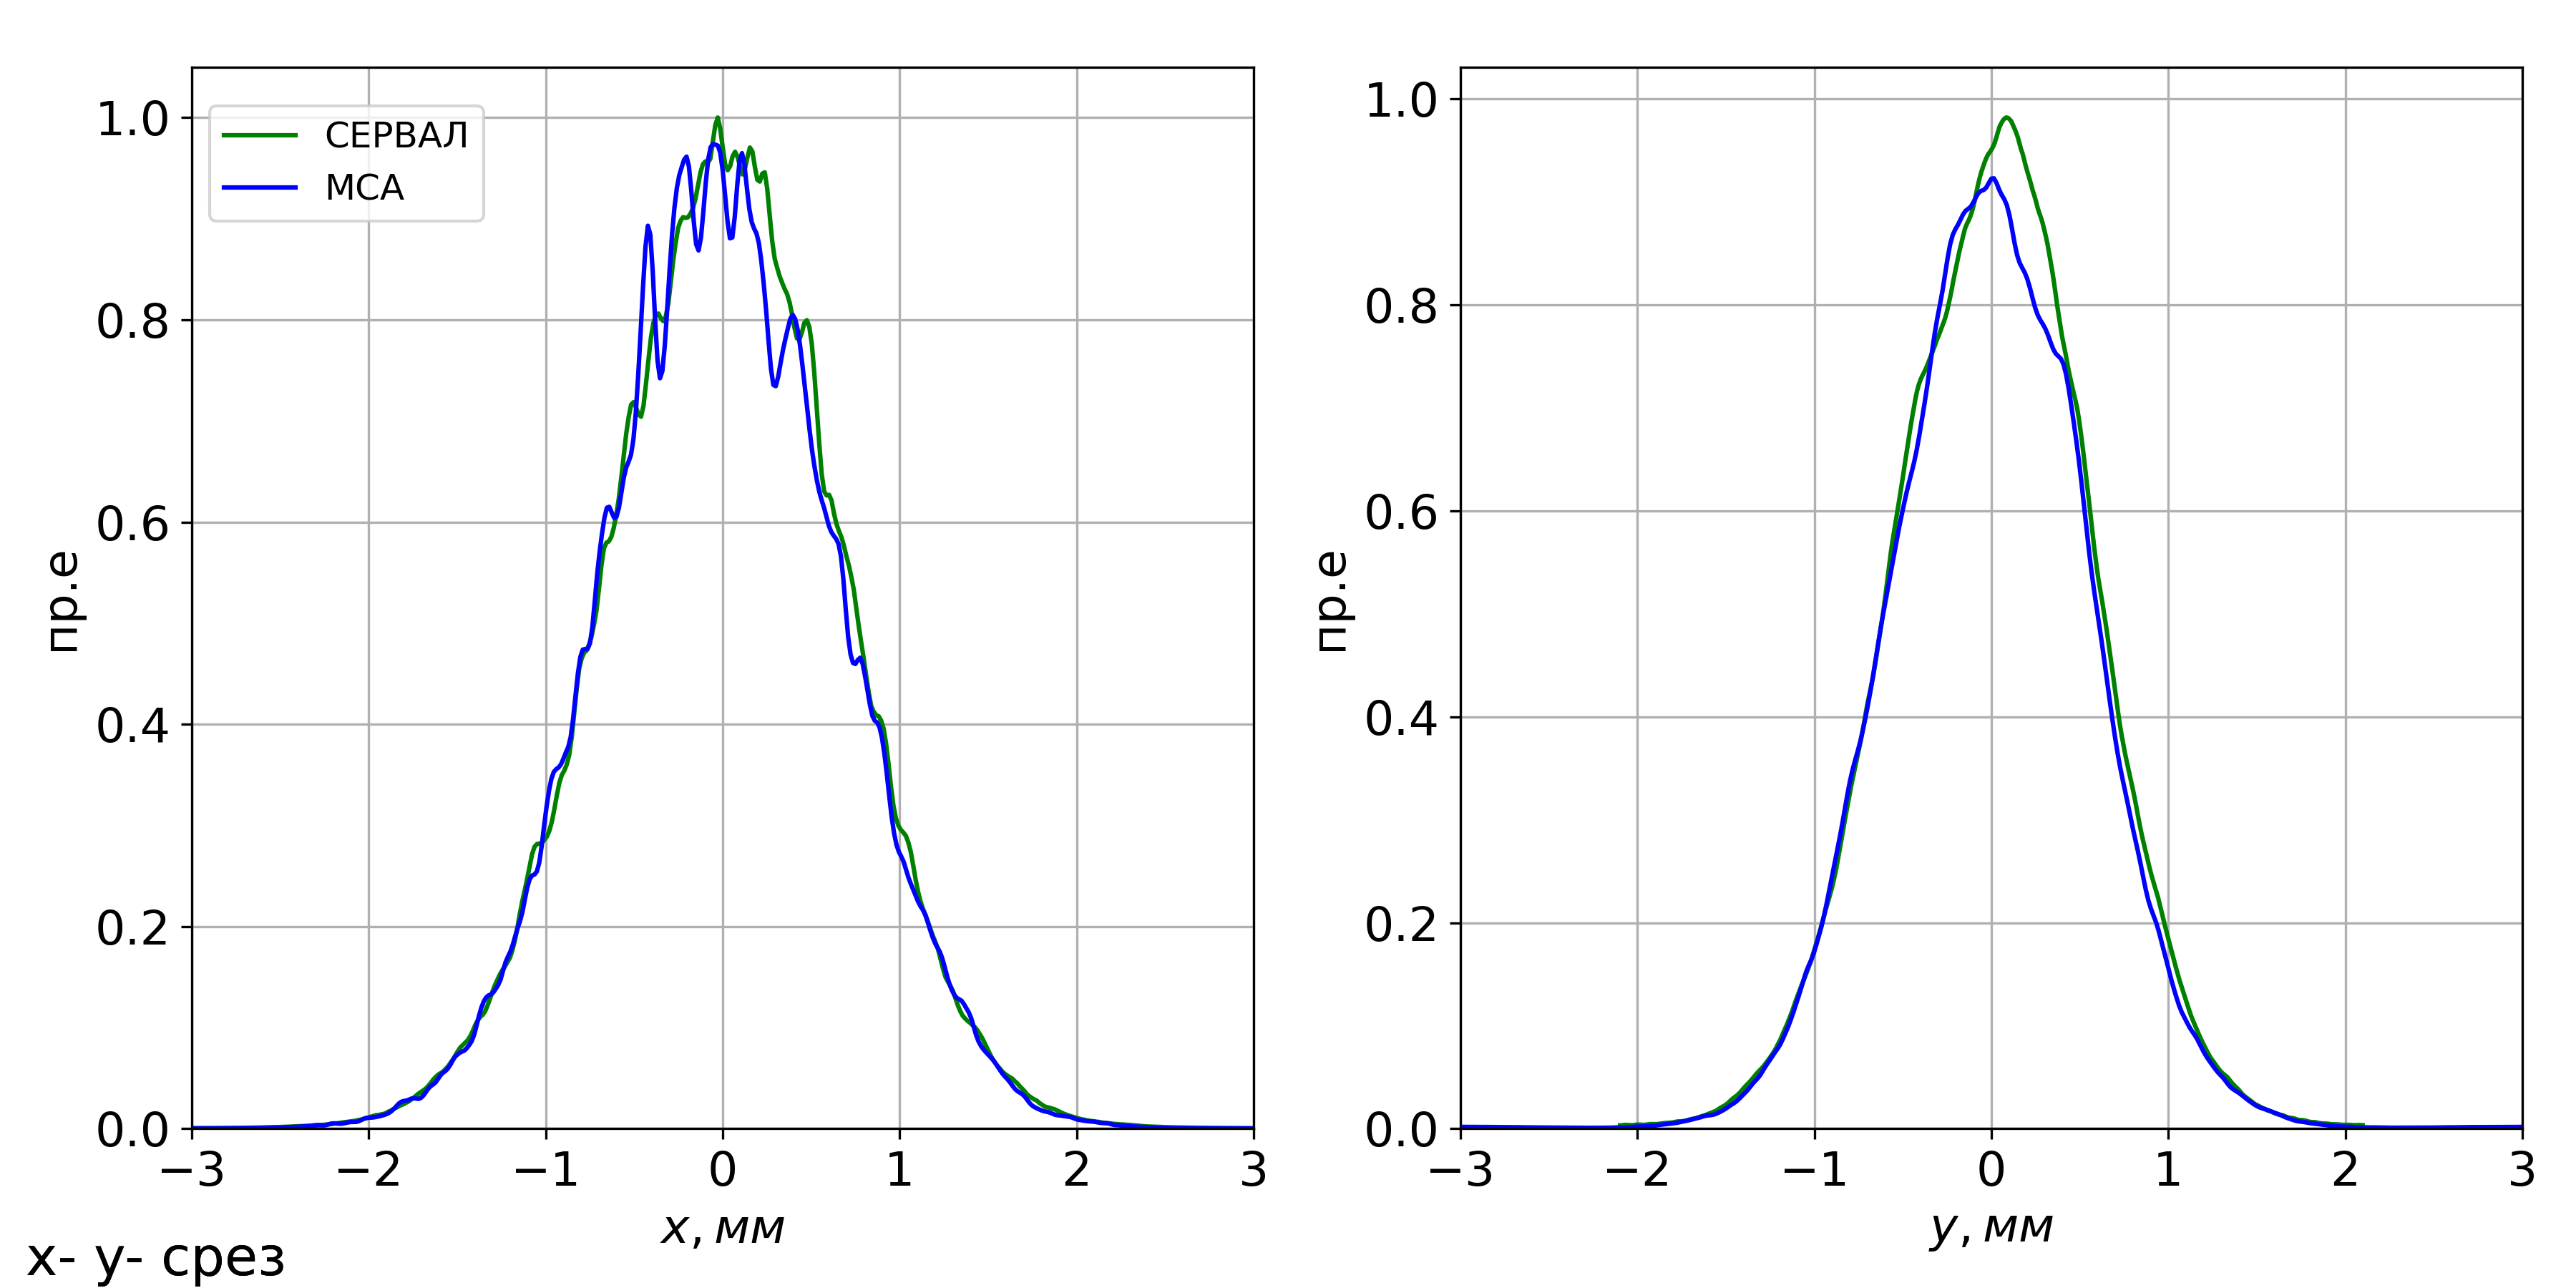
\includegraphics[width=0.99\linewidth]{SERVAL_envelopes_comparison_far_zone.png}
	\caption{Распределением на источнике \rr{перерисовать с большей плотностью точек и другими цветами линий}}
	\label{fig:diff_coh_incoh_rad}
\end{figure}
В большинстве случаев можно выбирать свёртку интенсивностей по~\ref{intensity}. Однако, стоит отметить, что SERVAL -- это оценочный метод и в случаее дифракционного ограниченного источника необходимо перед проведением расчётов сделать подобный анализ подходящих огибающих. 

\chapter{Применение СЕРВАЛа} \label{chapt3}
СЕРВАЛ является эффективным алгоритмом для моделирования частично когерентного синхротронного излучения, в случаях когда есть заметная степень когерентности источника излучения. Уже было показано совпадение распределений интенсивности в дальней зоне и на источнике излучения, а так же совпадение корреляционных функций с методом сложения амплитуд, который может считаться методом, дающий результат «из первых принципов» во всех ситуациях\footnote{необходимо помнить, что число $N_e$ должно быть достаточно велико для получения достоверного результата}. Этот сравнительный анализ свойств источника излучения даёт все предпосылки, что весьма ресурсозатратный по времени метод сложения амплитуд может быть заменён СЕРВАЛом без потери точности и физичности результатов. В этой главе мы приведём ещё один сравнительный анализ СЕРВАЛа и метода сложения амплитуд на примере фокусирующей системы с конечной апертурой, а так же два практических применения СЕРВАЛа на примере простого эксперимента Юнга и нетривиальной задачи отражения частично когерентного излучения от рентгеновского зеркала с шероховатостями. Расчёты будут проводиться для параметров электронного пучка ЦКП «СКИФ», которые представлены в Таблице~\ref{tab:SKIF parameters}
\begin{table}[H]
	\caption{Параметры ондулятора}
	\label{tab:undulator_parameters}	
	\begin{tabular}{l|c|r}	
		$E_{ph},  [\textup{эВ}]/\lambda, [\textup{\AA}$]& $\lambda_w, [\textup{mm}]$ & $L, [\textup{m}]$\\ 
		\hline	%0.65-1.35
		2167/5.72    &  18      & 3.6   
	\end{tabular}
\end{table}
В работе использовались следующий параметры ондулятора~\ref{tab:undulator_parameters}
\begin{table}[H]
	\caption{Параметры электронного пучка}
	\label{tab:SKIF parameters}	
	\begin{tabular}{l|c|c|c|r}
		$E, \textup{[GeV]}$ & $\sigma_x, \textup{[мкм]}$ & $\sigma_y, \textup{[мкм]}$ & $\sigma_{x'}, \textup{[мкрад]}$ & $\sigma_{y'}, \textup{[мкрад]}$ \\ 
		\hline
		3          &38                          & 4.7                        & 25                          & 20 
	\end{tabular}
\end{table} 
Однако, отдельно необходимо отметить, когда источник дифракционно ограничен, целесообразно применять метод сложения амплитуд или метод сложения интенсивностей, которые очень быстро дадут сходимость. В этом случае для СЕРВАЛа потребуется тщательный анализ подходящих огибающих и, строго говоря, метод \textit{не моделируют} фундаментальную моду ондуляторного излучения -- случай излучения электронного пучка с бесконечно малым эмиттансом\footnote{случай, когда эмиттанс излучения много больше эмиттанса электронного пучка}. Для источников с низкой степенью когерентности имеет смысл рассмотреть метод трассировки лучей, в этом случае все три волновых метода будут иметь весьма низкую сходимость и придётся моделировать большое число статистических реализаций для получения сходимости. В любом случае, в каждом из рассмотренных случаев прежде чем проводить оптический расчёт, необходимо изучить свойства источника излучения, например при помощи программы SPECTRA~\cite{tanaka_spectra_2001}, оценить ожидаемую степень когерентности и только исходя из свойств источника применять один из описанных методов моделирования. Именно такой подход даст оптимальный результат в смысле затраченного времени и физичности полученных результатов. 

\section{Фокусирующая система с конечной апертурой}\label{section:focusing_system_with_aperture}
Рассмотрим оптическую систему состоящую из источника излучения -- ондулятора, апертуры и фокусирующего элемента. Для SERVAL были выбраны огибающие~\ref{intensity}. Этот расчёт будет сопровождаться сравнением результатов метода СЕРВАЛ с результатами метода сложения амплитуд (МСА).

\begin{figure}[H] 
	\centering 	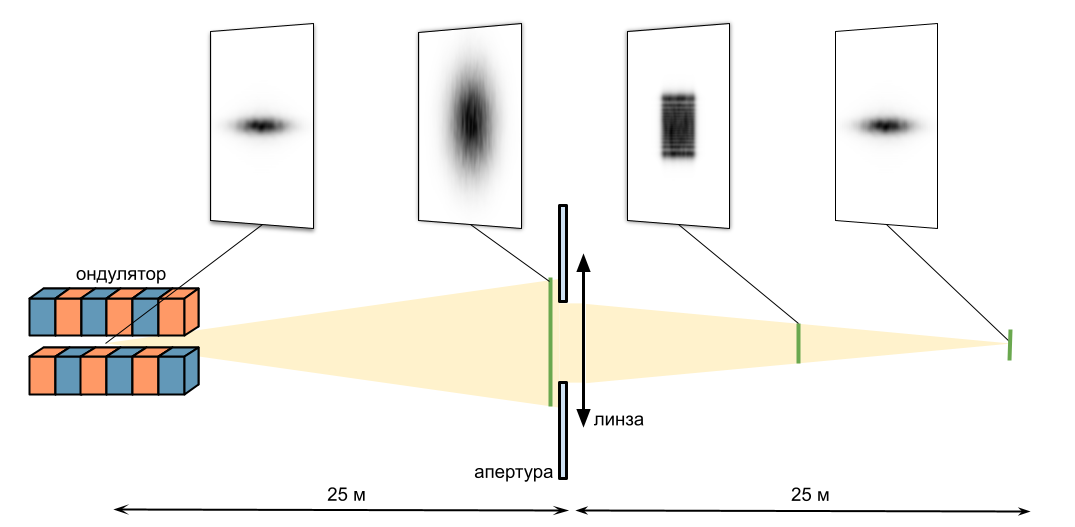
\includegraphics[width=0.99\linewidth]{beamline.png}
	\caption{Схема оптики}
	\label{fig:beamline}
\end{figure}
Распределение поля в дальней зоне на 25 м от ондулятора представлено на Рис.~\ref{fig:focusing_system_far_zone}.
\begin{figure}[H] 
	\centering 	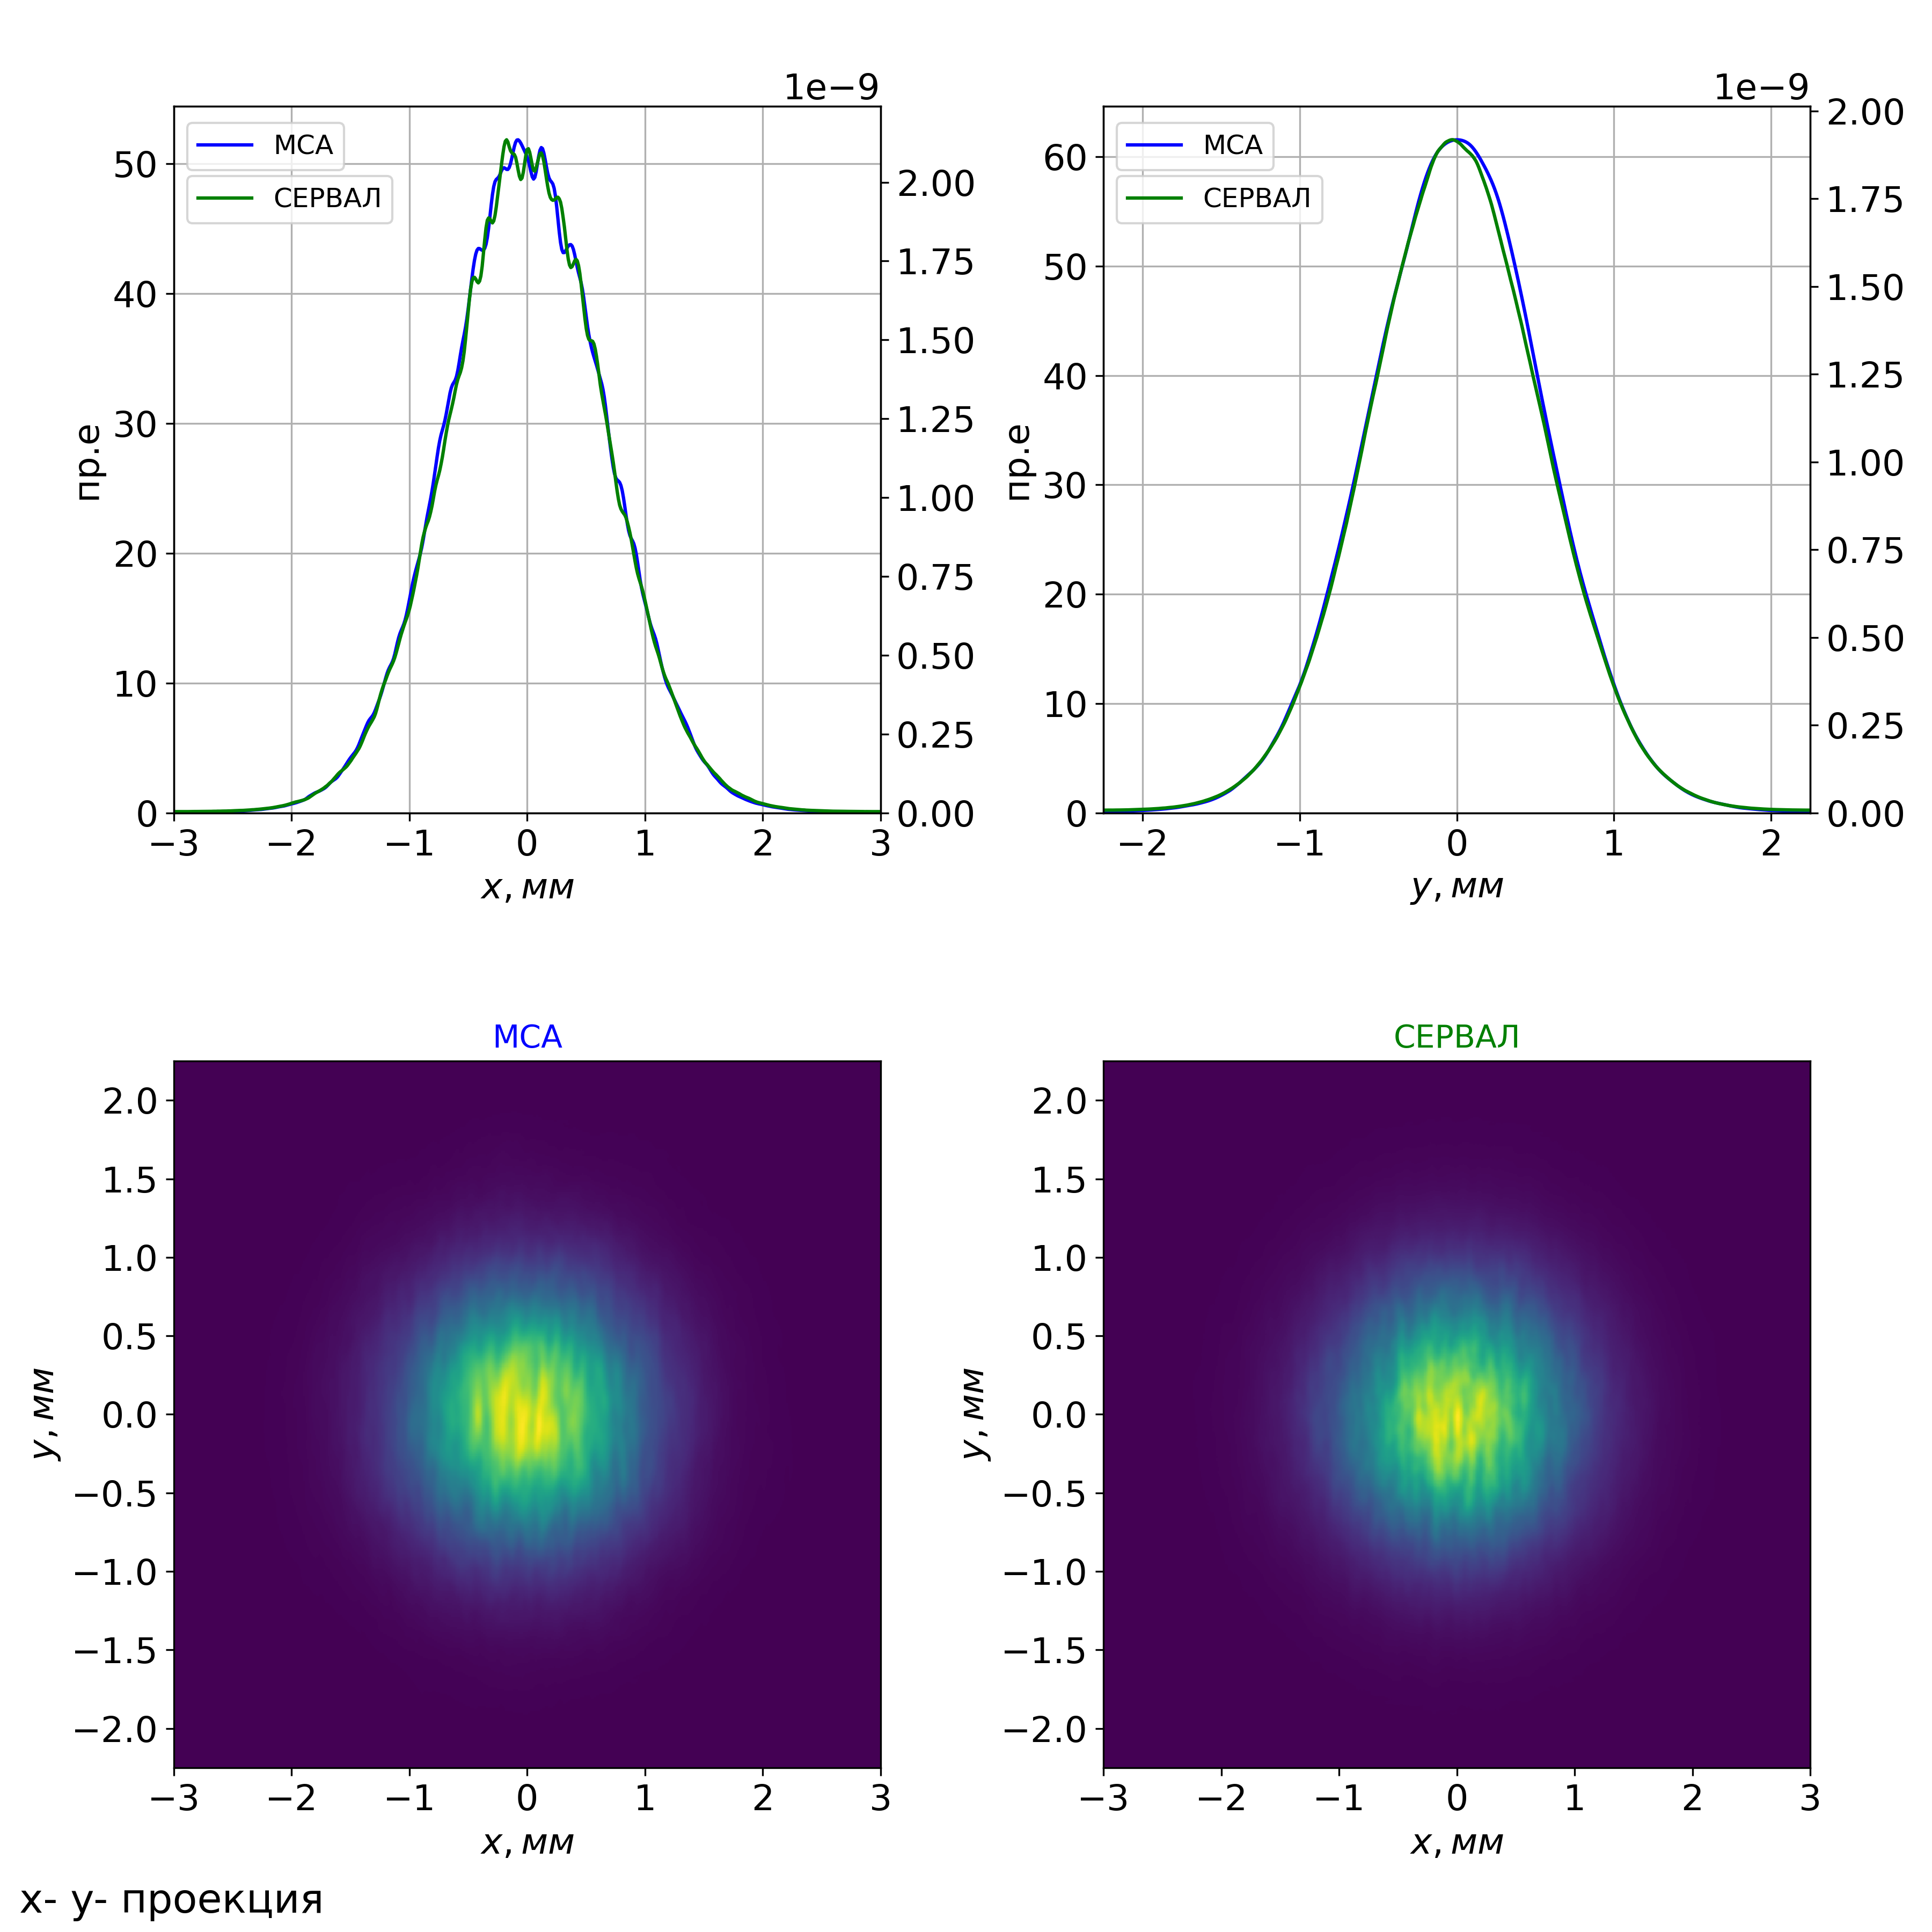
\includegraphics[width=0.99\linewidth]{1-far_zone_25_m3.80E-05_um_4.68E-06_um_2.50E-05_urad_2.00E-05_urad_example_beamline.png}
	\caption{Распределение интенсивности излучения в дальней зоне. \rr{$MCA_x, СЕРВАЛ_x = 1500$ мкм, $MCA_x, СЕРВАЛ_x = 1270$ мкм}}
	\label{fig:focusing_system_far_zone}
\end{figure}
Для усреднения было выбрано 300 реализаций, что даёт достаточную сходимость. Однако в структуре излучения всё ещё видна характерная модовая структура. Видно что количество мод в вертикальном направление меньше чем в горизонтальном, а их типичный размер говорит о длине поперечной когерентности в соответствующих направлениях. Размер пятна когерентности определяется через размер функции взаимной когерентности, представленной на Рис.~\ref{fig:focusing_system_corr}.
\begin{figure}[H] 
	\centering 	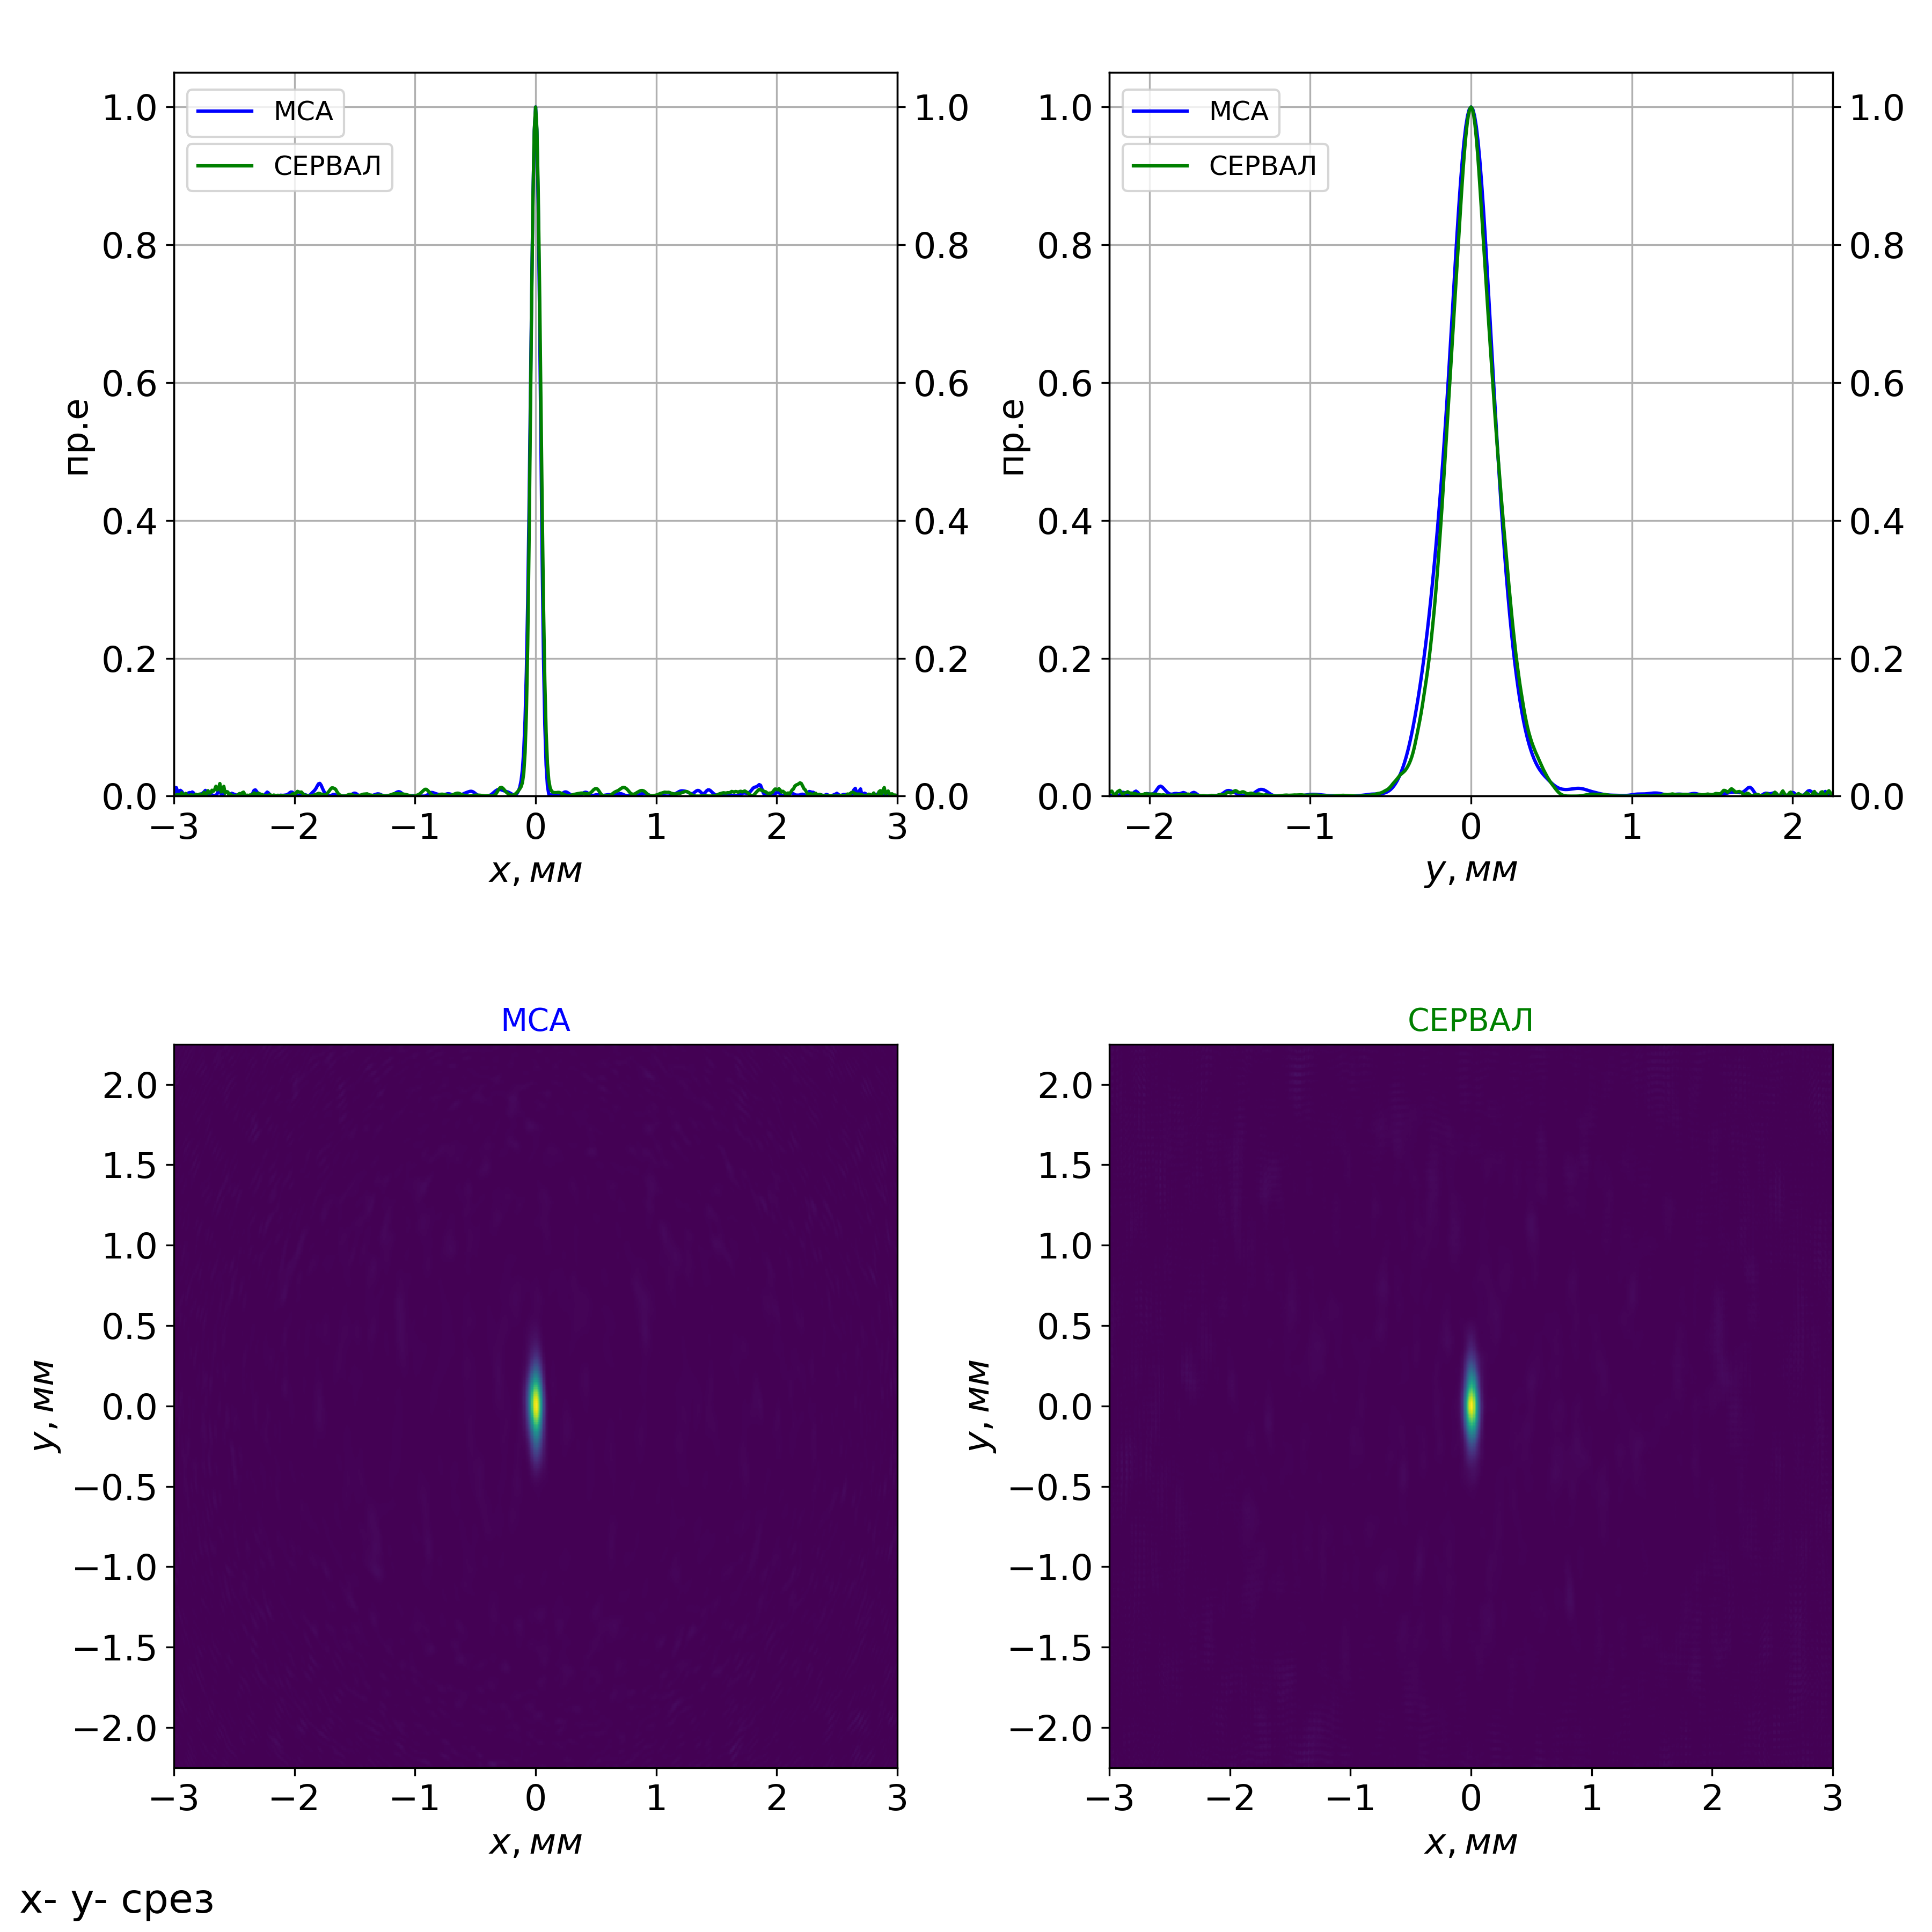
\includegraphics[width=0.99\linewidth]{corr3.80E-05_um_4.68E-06_um_2.50E-05_urad_2.00E-05_urad_example_beamline.png}
	\caption{Корреляционная функция, построенная по формуле~\ref{eq:g1}. \rr{$MCA_x, СЕРВАЛ_x = 87$ мкм, $MCA_x, СЕРВАЛ_x = 320$ мкм}}
	\label{fig:focusing_system_corr}
\end{figure}
\noindent После апертуры и 10 метров распространения поля через пустое пространство результат приведён на Рис.~\ref{fig:focusing_system_far_zone}
\begin{figure}[H] 
	\centering 	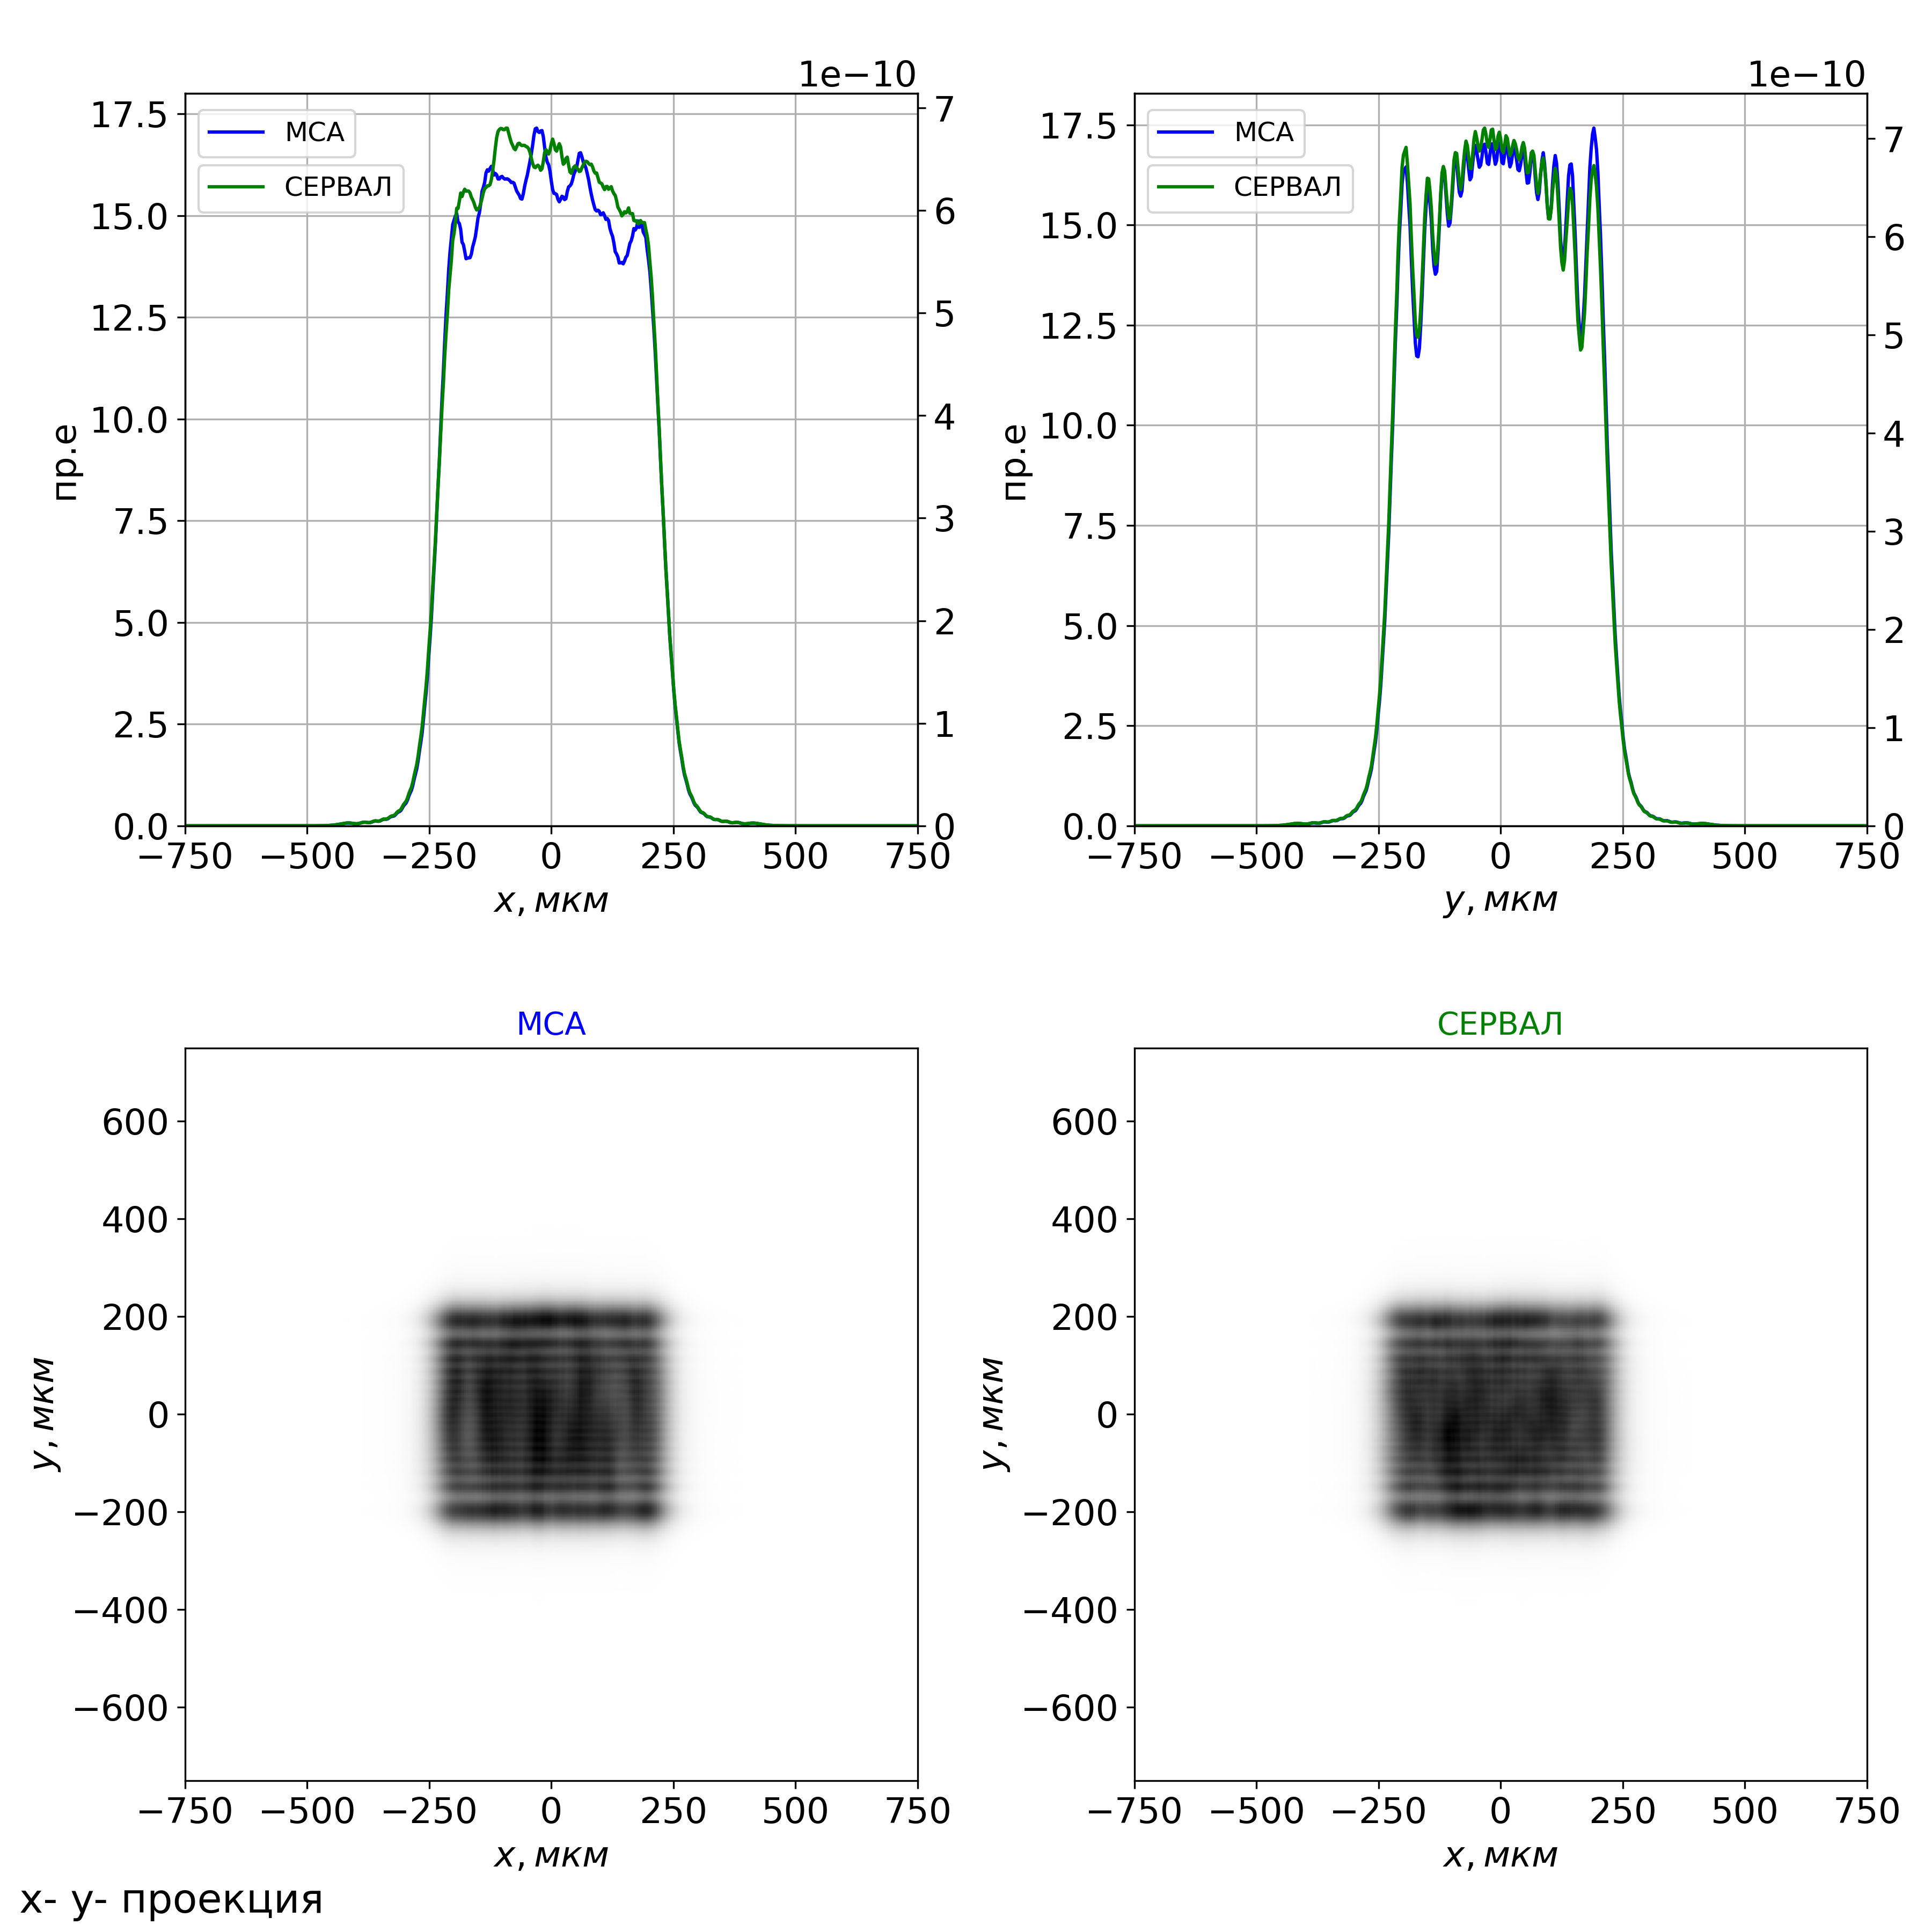
\includegraphics[width=0.99\linewidth]{2-far_zone_12_5_m_after_aperture3.80E-05_um_4.68E-06_um_2.50E-05_urad_2.00E-05_urad_example_beamline.png}
	\caption{\rr{$MCA_x, СЕРВАЛ_x = 453$ мкм, $MCA_x, СЕРВАЛ_x = 445, 442$ мкм}}
	\label{fig:focusing_system_after_aperture}
\end{figure}
\noindent Дифракционные картины отличаются для каждого из направлений, для вертикального дифракционные пики более выраженные ввиду большей длины когерентности, для горизонтального направления заметен только первый дифракционный максимум, что говорит о заметно меньшей степени когерентности.

Распределение поля в фокальной плоскости приведено на Рис.~\ref{fig:focusing_system_in_focus}.
\begin{figure}[H] 
	\centering 	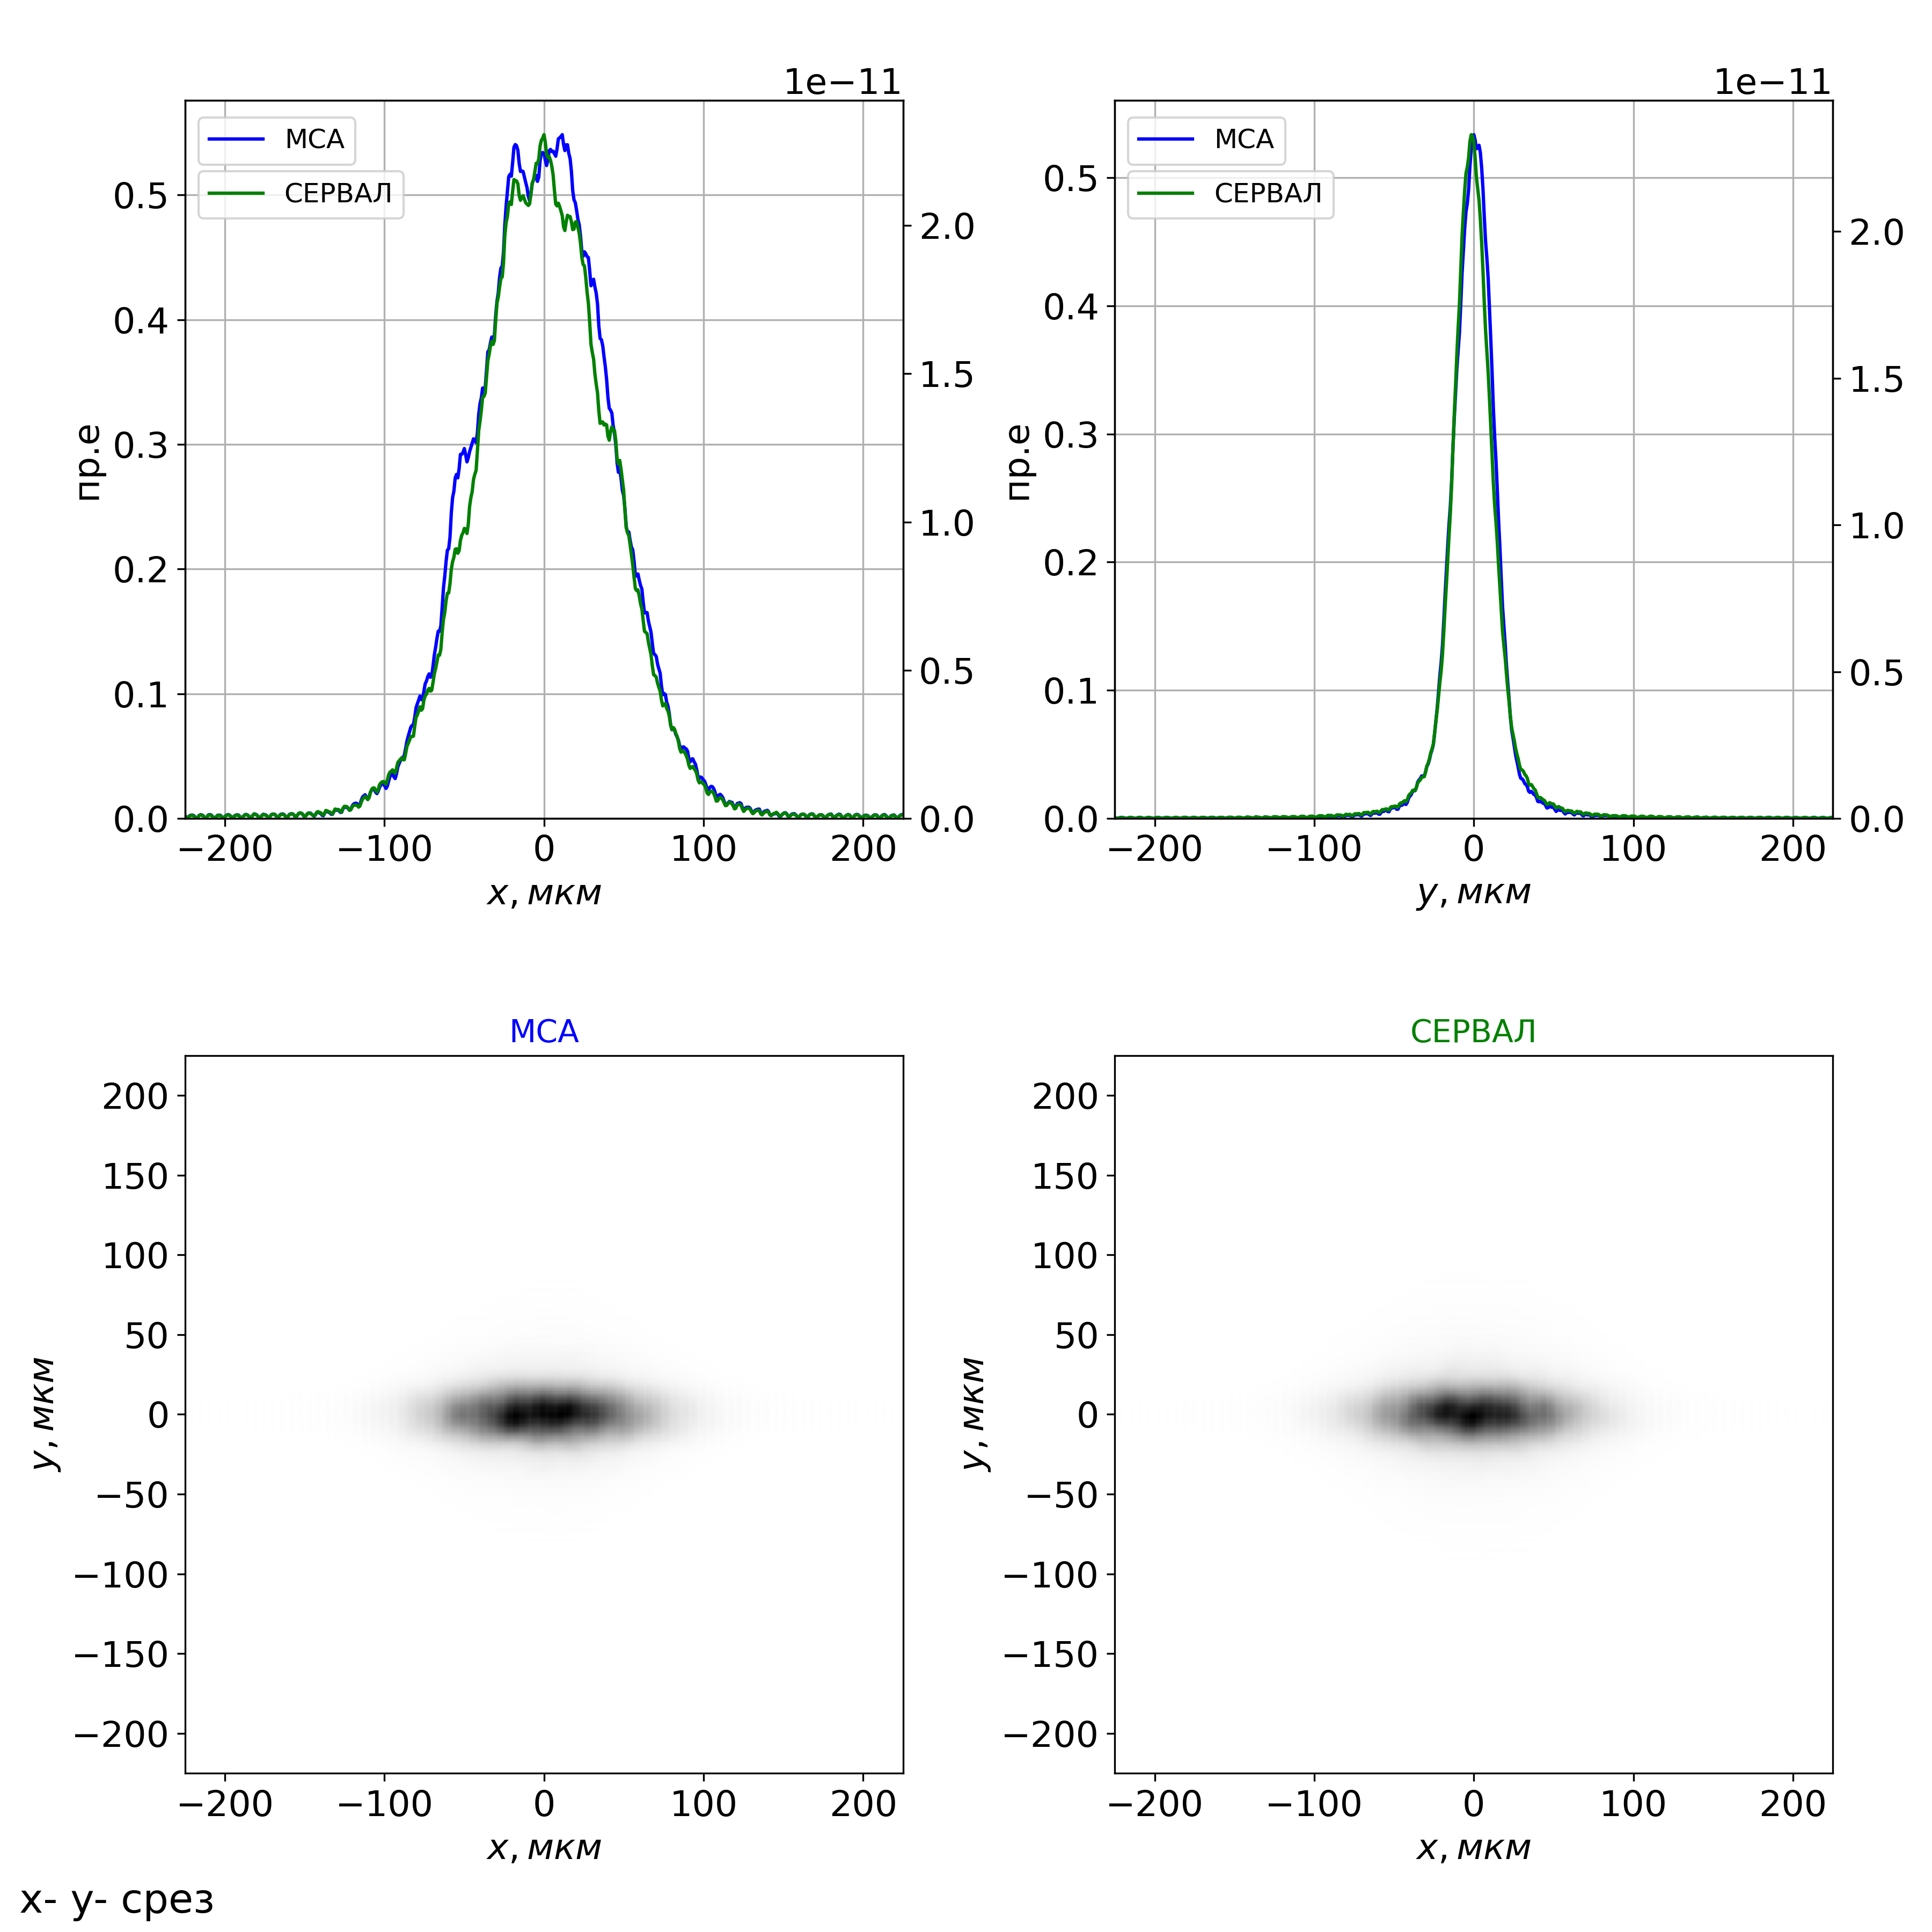
\includegraphics[width=0.99\linewidth]{3-70_m_focal_plane3.80E-05_um_4.68E-06_um_2.50E-05_urad_2.00E-05_urad_example_beamline.png}
	\caption{Распределение излучения в фокусе \rr{$MCA_x, СЕРВАЛ_x = 100$ мкм, $MCA_x, СЕРВАЛ_x = 26$ мкм}}
	\label{fig:focusing_system_in_focus}
\end{figure}
\noindent Для моделирования было выбрано соотношение плеч фокусирующей системы -- $1:1$. В горизонтально направлении источник можно считать гауссовым с полной шириной на полувысоте $80$ мкм, после фокусировки мы видим уширение изображения до $100$ мкм, которое приходит из-за апертуры и намного меньшее уширение в вертикальном направлении до $26$ мкм при истинном размере источника $24$ мкм. По критерию Релея $\theta_{diff} = 1.22 \lambda / D$, где $D$ размер апертуры, -- дифракционный предел для обоих направлений $0.7$ мкрад при видимом размере источника для горизонтального направления $3.2$ мкрад и $0.96$ мкрад -- для вертикального. Видно, что для горизонтального направления та же апертура будет вносить больший вклад в увеличение размера фокусного пятна.
\rr{заключение}
\section{Интерференционный эксперимент}
Чтобы наглядно продемонстрировать эффекты, связанные с частичной когерентностью, показательно будет провести классический опыт Юнга (двухщелевой интерферометр Юнга). Ниже на Рис.~\ref{fig:x_field_before_slit} и~\ref{fig:x_corr_before_slit} опять же приведён размер излучения на $25$ м от источника излучения и распределение корреляционной функции в увеличенном масштабе с наложенными щелями. Щели на рисунках обозначены зелёным цветом -- с межщелевым зазором $75$ мкм, красным -- $150$ мкм и оранжевым $300$ мкм, при характерном размере корреляционной функции полной шириной на половине высоты (ПШПВ) $87 \times 320$ $\textup{мкм}^2$. 
\begin{figure}[H]
	\centering
	\begin{minipage}{0.33\textwidth}
		\centering
		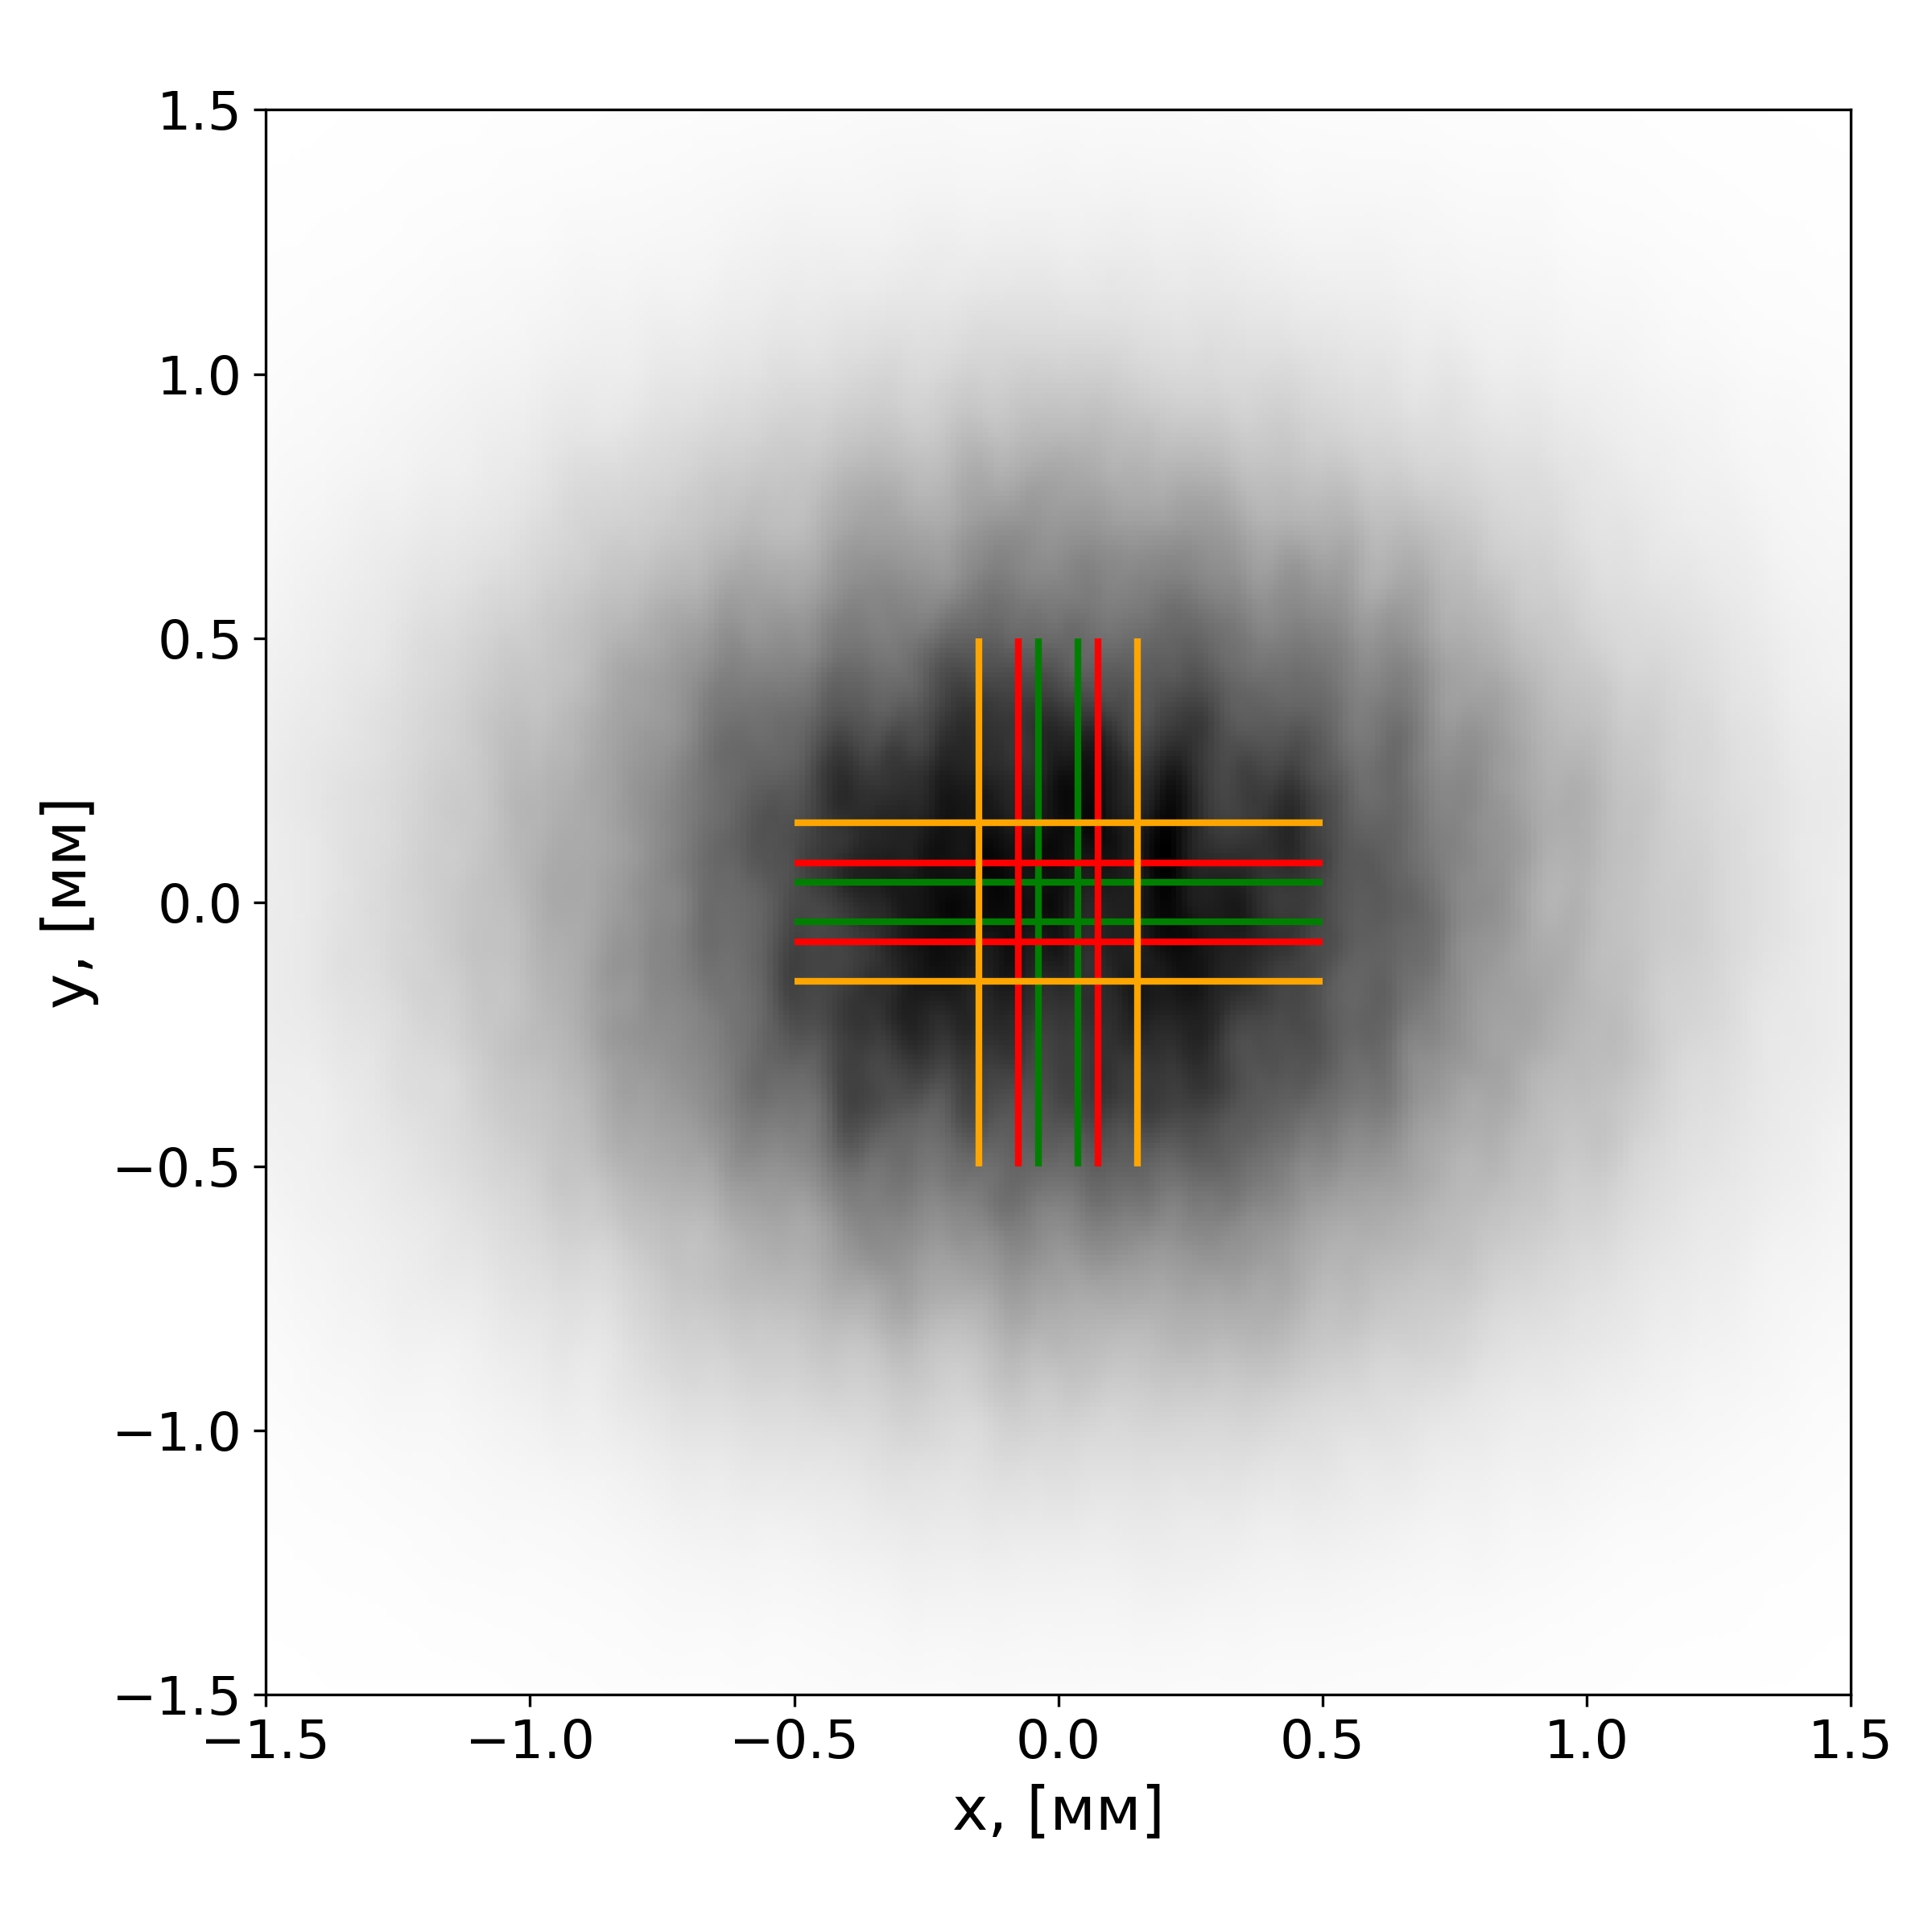
\includegraphics[width=1\linewidth]{field_before_slit.png}
		\caption{Размер излучения на $25$ м от источника с щелями, обозначенными цветными полосками  \rr{убрать горизонтальные полоски}}
		\label{fig:x_field_before_slit}
	\end{minipage}
	\begin{minipage}{0.33\textwidth}
		\centering
		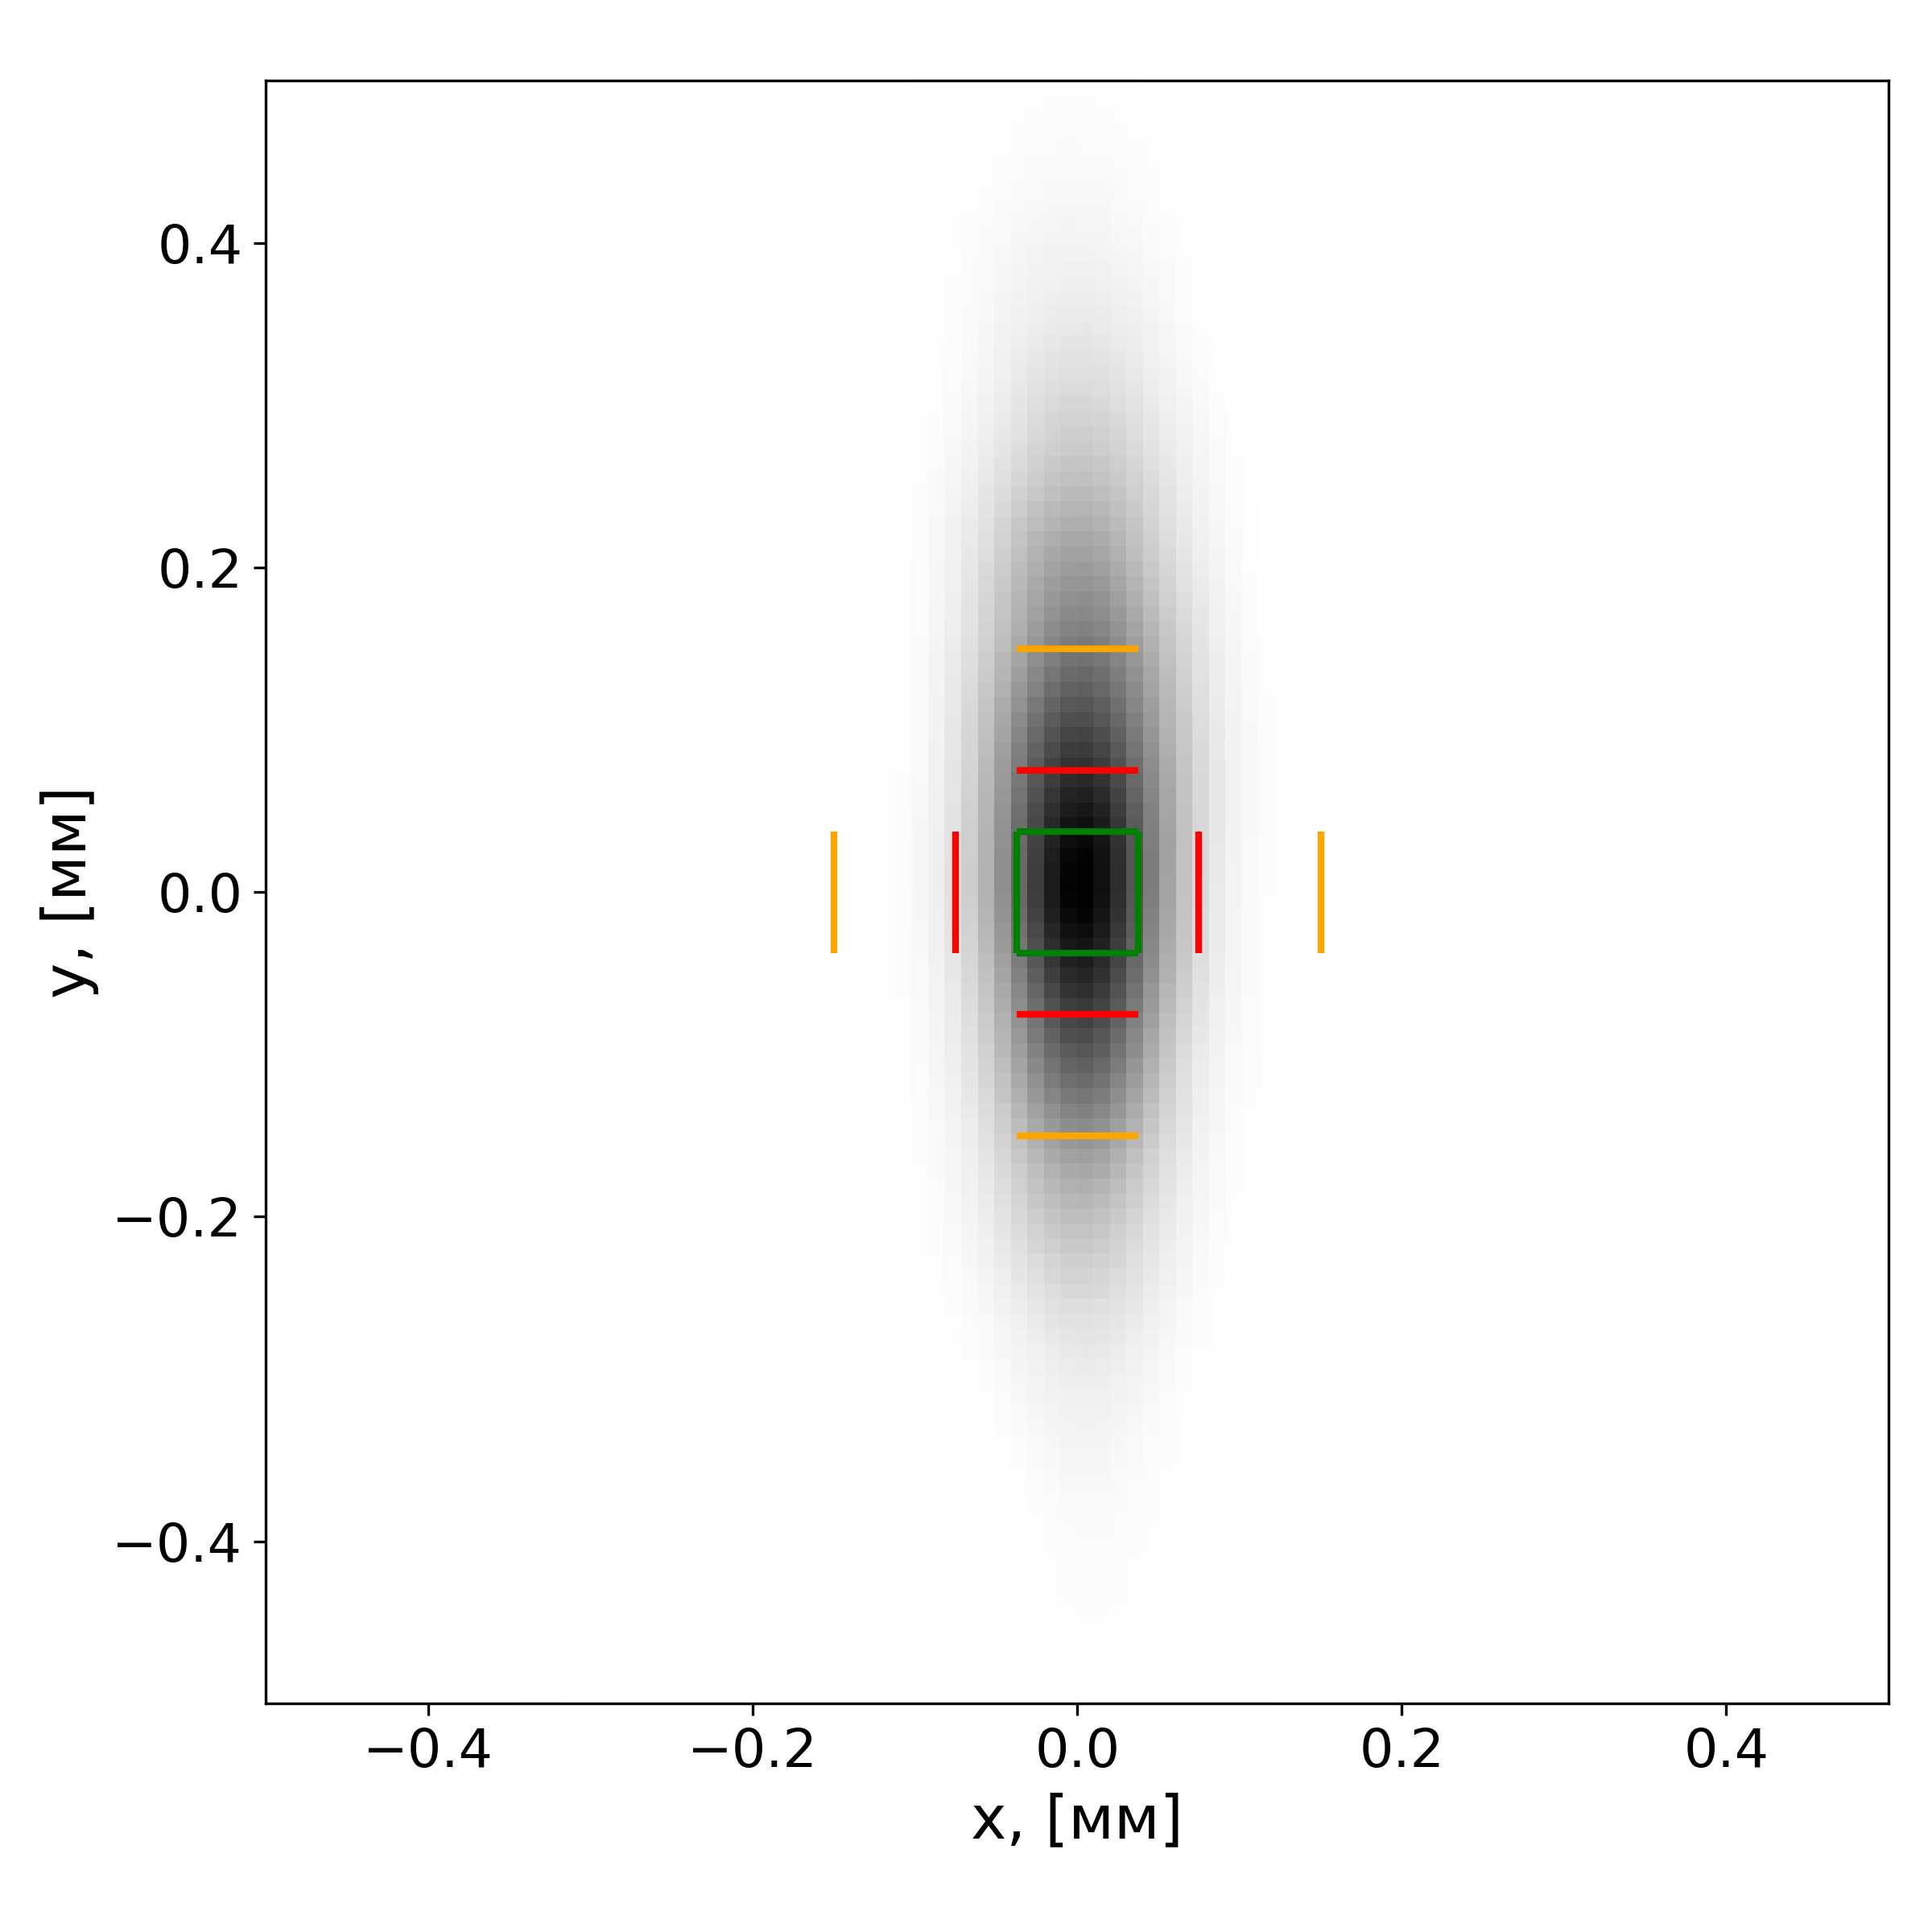
\includegraphics[width=1\linewidth]{corr_before_slit.png}
		\caption{Пятно когерентности на $25$ м от источника с щелями, обозначенными цветными полосками \rr{убрать горизонтальные полоски}}
		\label{fig:x_corr_before_slit}
	\end{minipage}\hfill
\end{figure}
\noindent Для начала продемонстрируем интерференционную картину отдельно от каждой из реализации и получившееся усреднённое по реализациям изображение, представленные на Рис.~\ref{fig:double slit experiment} для вертикального расположения щелей с щелевым зазором $75$ мкм.
\begin{figure}[H] 
	\centering 	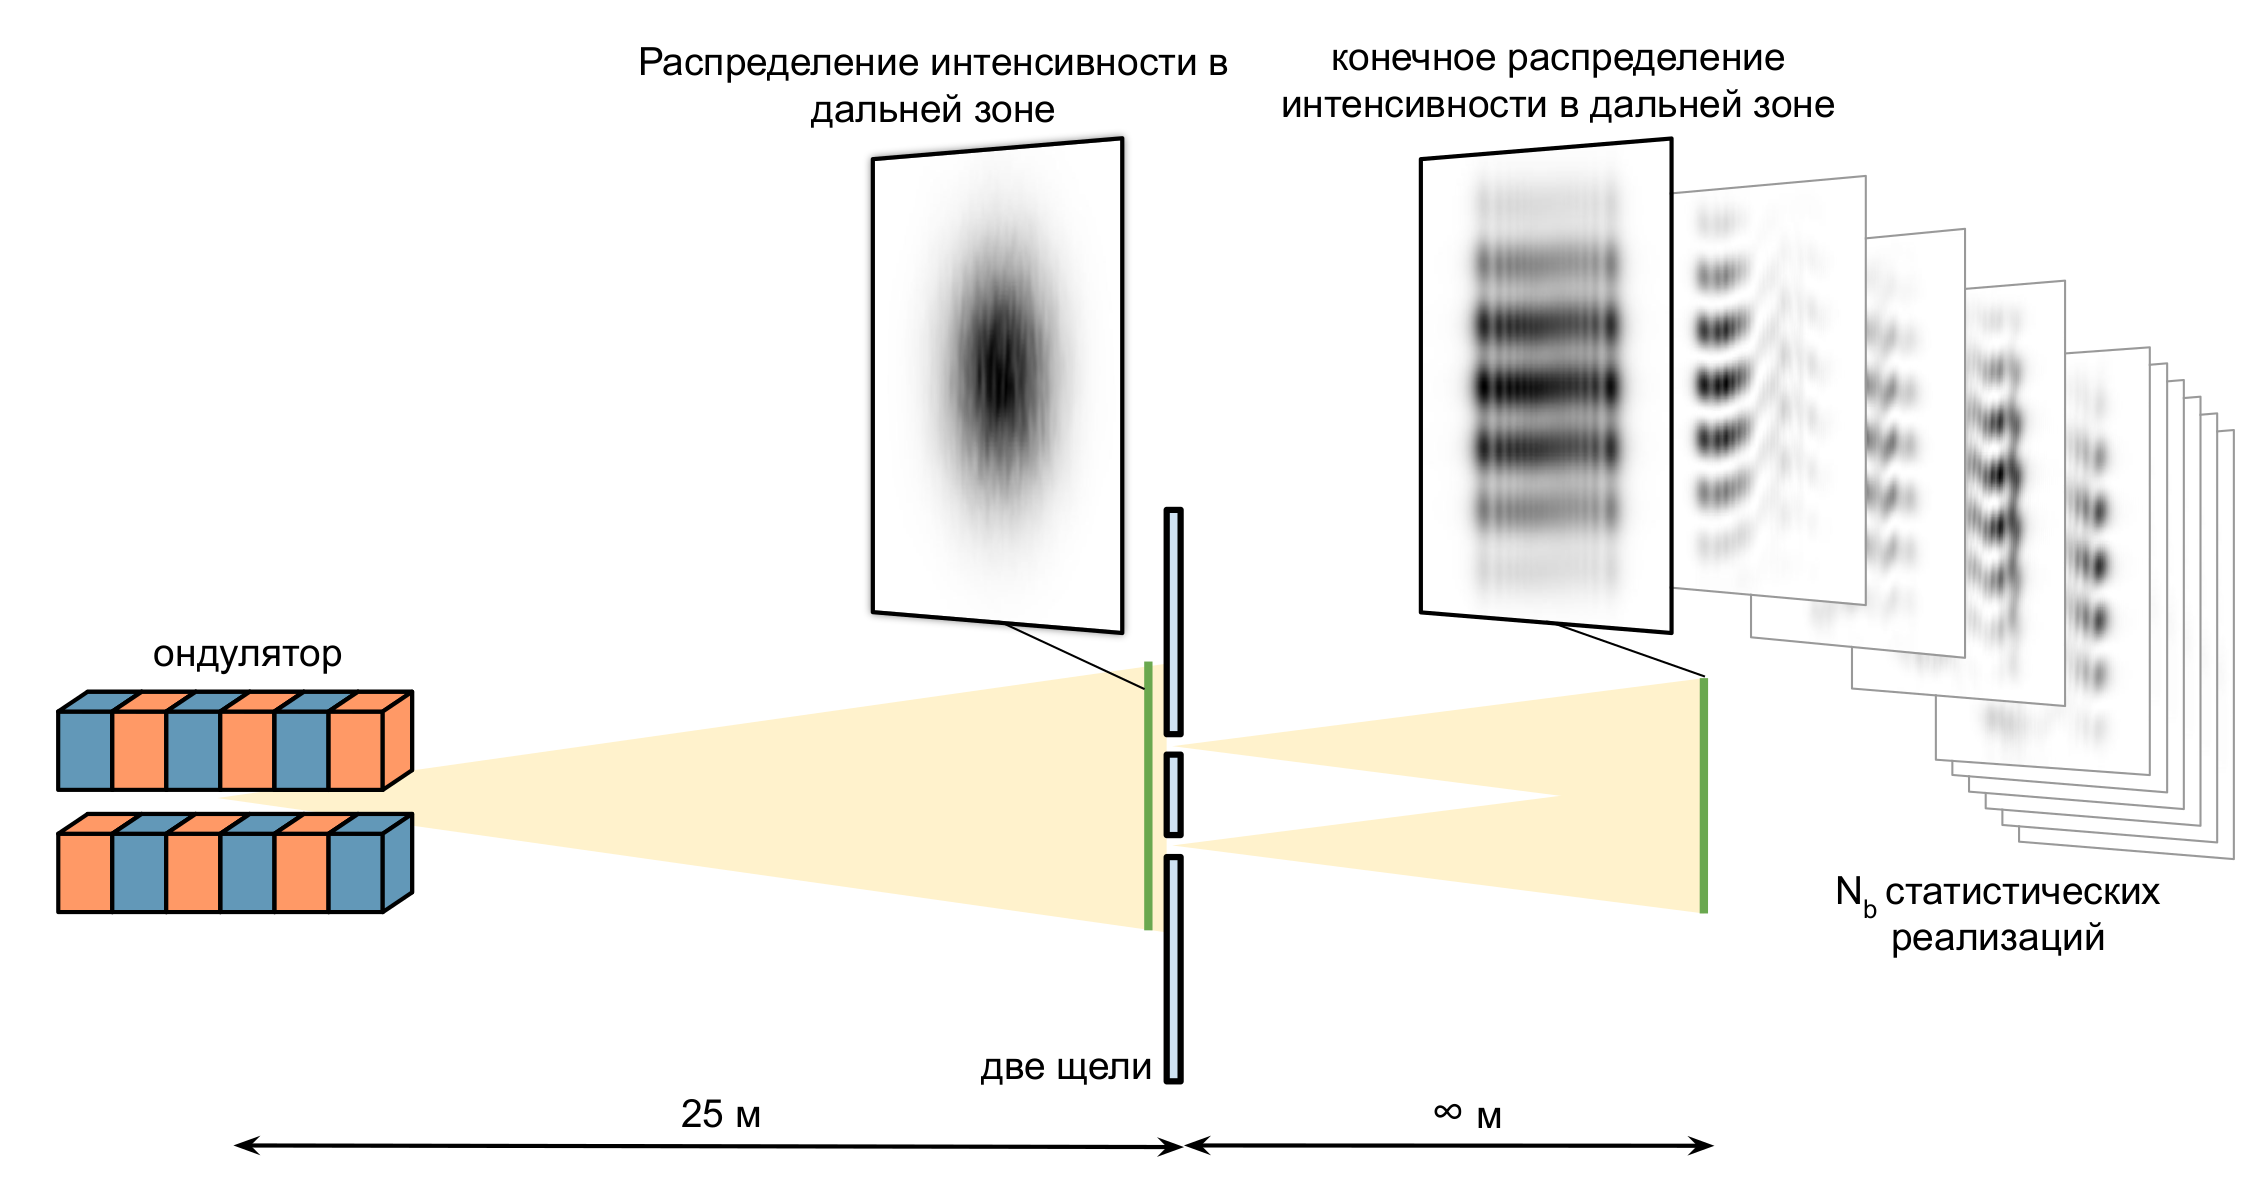
\includegraphics[width=0.99\linewidth]{double_slit_scheme.png}
	\caption{Схема двухщелевого эксперимента. После щелей -- интерферограмма усреднённая по 400 реализациям, а за ней интерферограммы для отдельных реализаций из этого статистического набора набора. Интерферограммы приведены в k-пространства сразу за щелями. Примечательно, что видность каждой из реализаций равна единице, но при усреднение по многим реализациям видность падает ввиду наличия частичной когерентности излучения]}
	\label{fig:double slit experiment}
\end{figure}
\noindent Дело в том, что «Хотя видность любой из этих отдельны интерферограмм соответствует значение $|\mu_{12}| = 1$\footnote{$\mu_{12}$ -- комплексный коэффициент когерентности, соответствующий $g^{(1)}$ в настоящей работе}, видность суперпозиции интерферограмм, вообще говоря, будет иной, поскольку фазы отдельных компонент будут изменяться от реализации к реализации. Таким образом, интерферограмма, усреднённая по ансамблю, вообще говоря, даст значения $|\mu_{12}|$, весьма отличные от единицы.», -- Дж. Гудмен, «Статистическая оптика», издательство «Мир», 1988, стр. $332-333$ или зарубежное издание~\cite{goodman_statistical_2015}.

Теперь можно представить усреднённые по реализациям интерферограммы для различных межщелевых расстояний, представленные на Рис.~\ref{fig:x_slits_75},~\ref{fig:x_slits_150},~\ref{fig:x_slits_300}. Указанные картины представлены для вертикального расположения щелей.
\begin{figure}[H]
	\centering
	\begin{minipage}{0.33\textwidth}
		\centering
		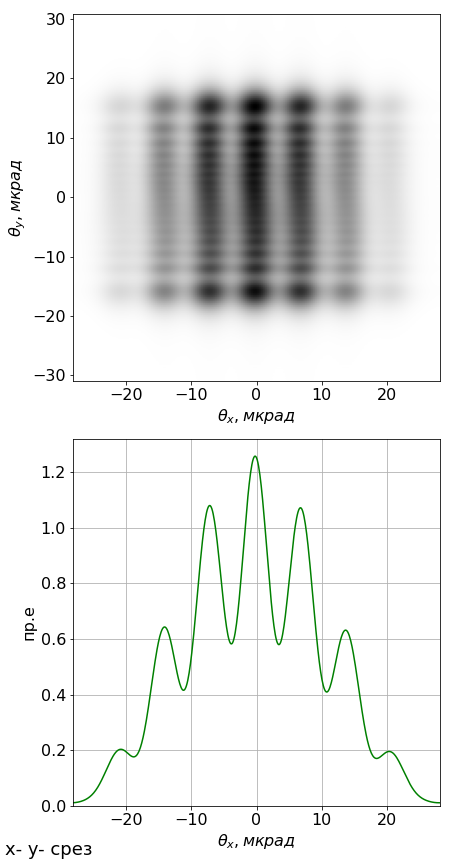
\includegraphics[width=1\linewidth]{x_slits_width_3e-05_separation_7.5e-05_.png}
		\caption{$75$ мкм}
		\label{fig:x_slits_75}
	\end{minipage}
	\begin{minipage}{0.33\textwidth}
		\centering
		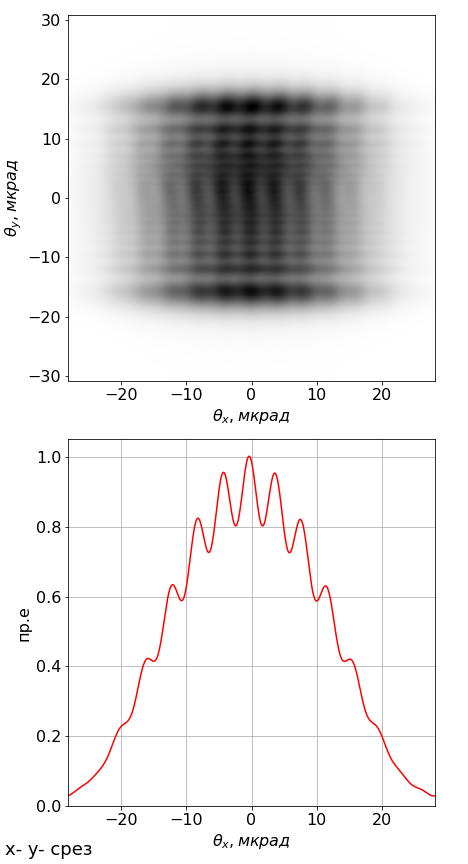
\includegraphics[width=1\linewidth]{x_slits_width_3e-05_separation_0.00015_.png}
		\caption{$150$ мкм}
		\label{fig:x_slits_150}
	\end{minipage}\hfill
	\begin{minipage}{0.33\textwidth}
		\centering
		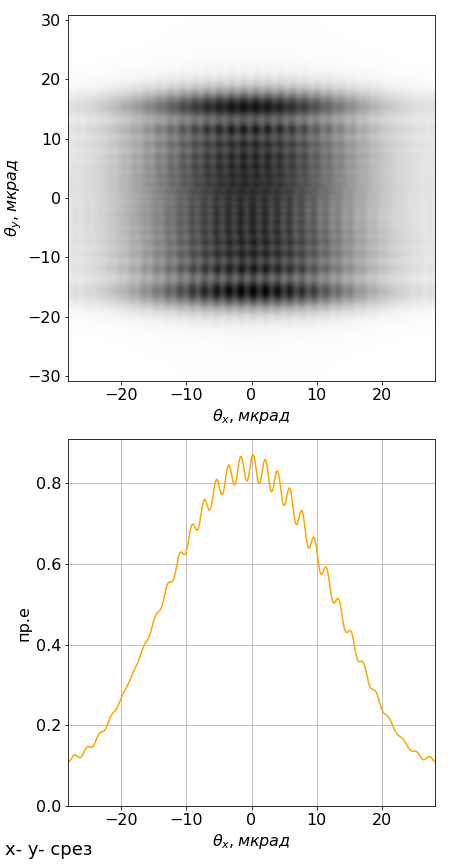
\includegraphics[width=1\linewidth]{x_slits_width_3e-05_separation_0.0003_.png}
		\caption{$300$ мкм}
		\label{fig:x_slits_300}
	\end{minipage}\hfill
\end{figure}
Примечательно заметить, что эти интерференционные картины представлены в $k$-пространстве или, другими словами, представлены в дальней зоне на достаточном расстоянии $z$ от щелей\footnote{так же именно такое изображение получится, если сразу за щелями поставить линзу, в фокусе будет соответствующая дифракционная картина}. Ещё одна особенность получившихся изображений: щели имеют конечный, в данном случае, горизонтальны размер равный $1$ мм, именно поэтому в вертикальном направлении на Рис.~\ref{fig:x_slits_75},~\ref{fig:x_slits_150},~\ref{fig:x_slits_300} видны характерные дифракционные картины от плоскости.

Аналогичные интерферограммы построены для вертикального направления, в котором излучение обладает большей когерентностью. Щели в данном случае ориентированны горизонтально.
\begin{figure}[H]
	\centering
	\begin{minipage}{0.33\textwidth}
		\centering
		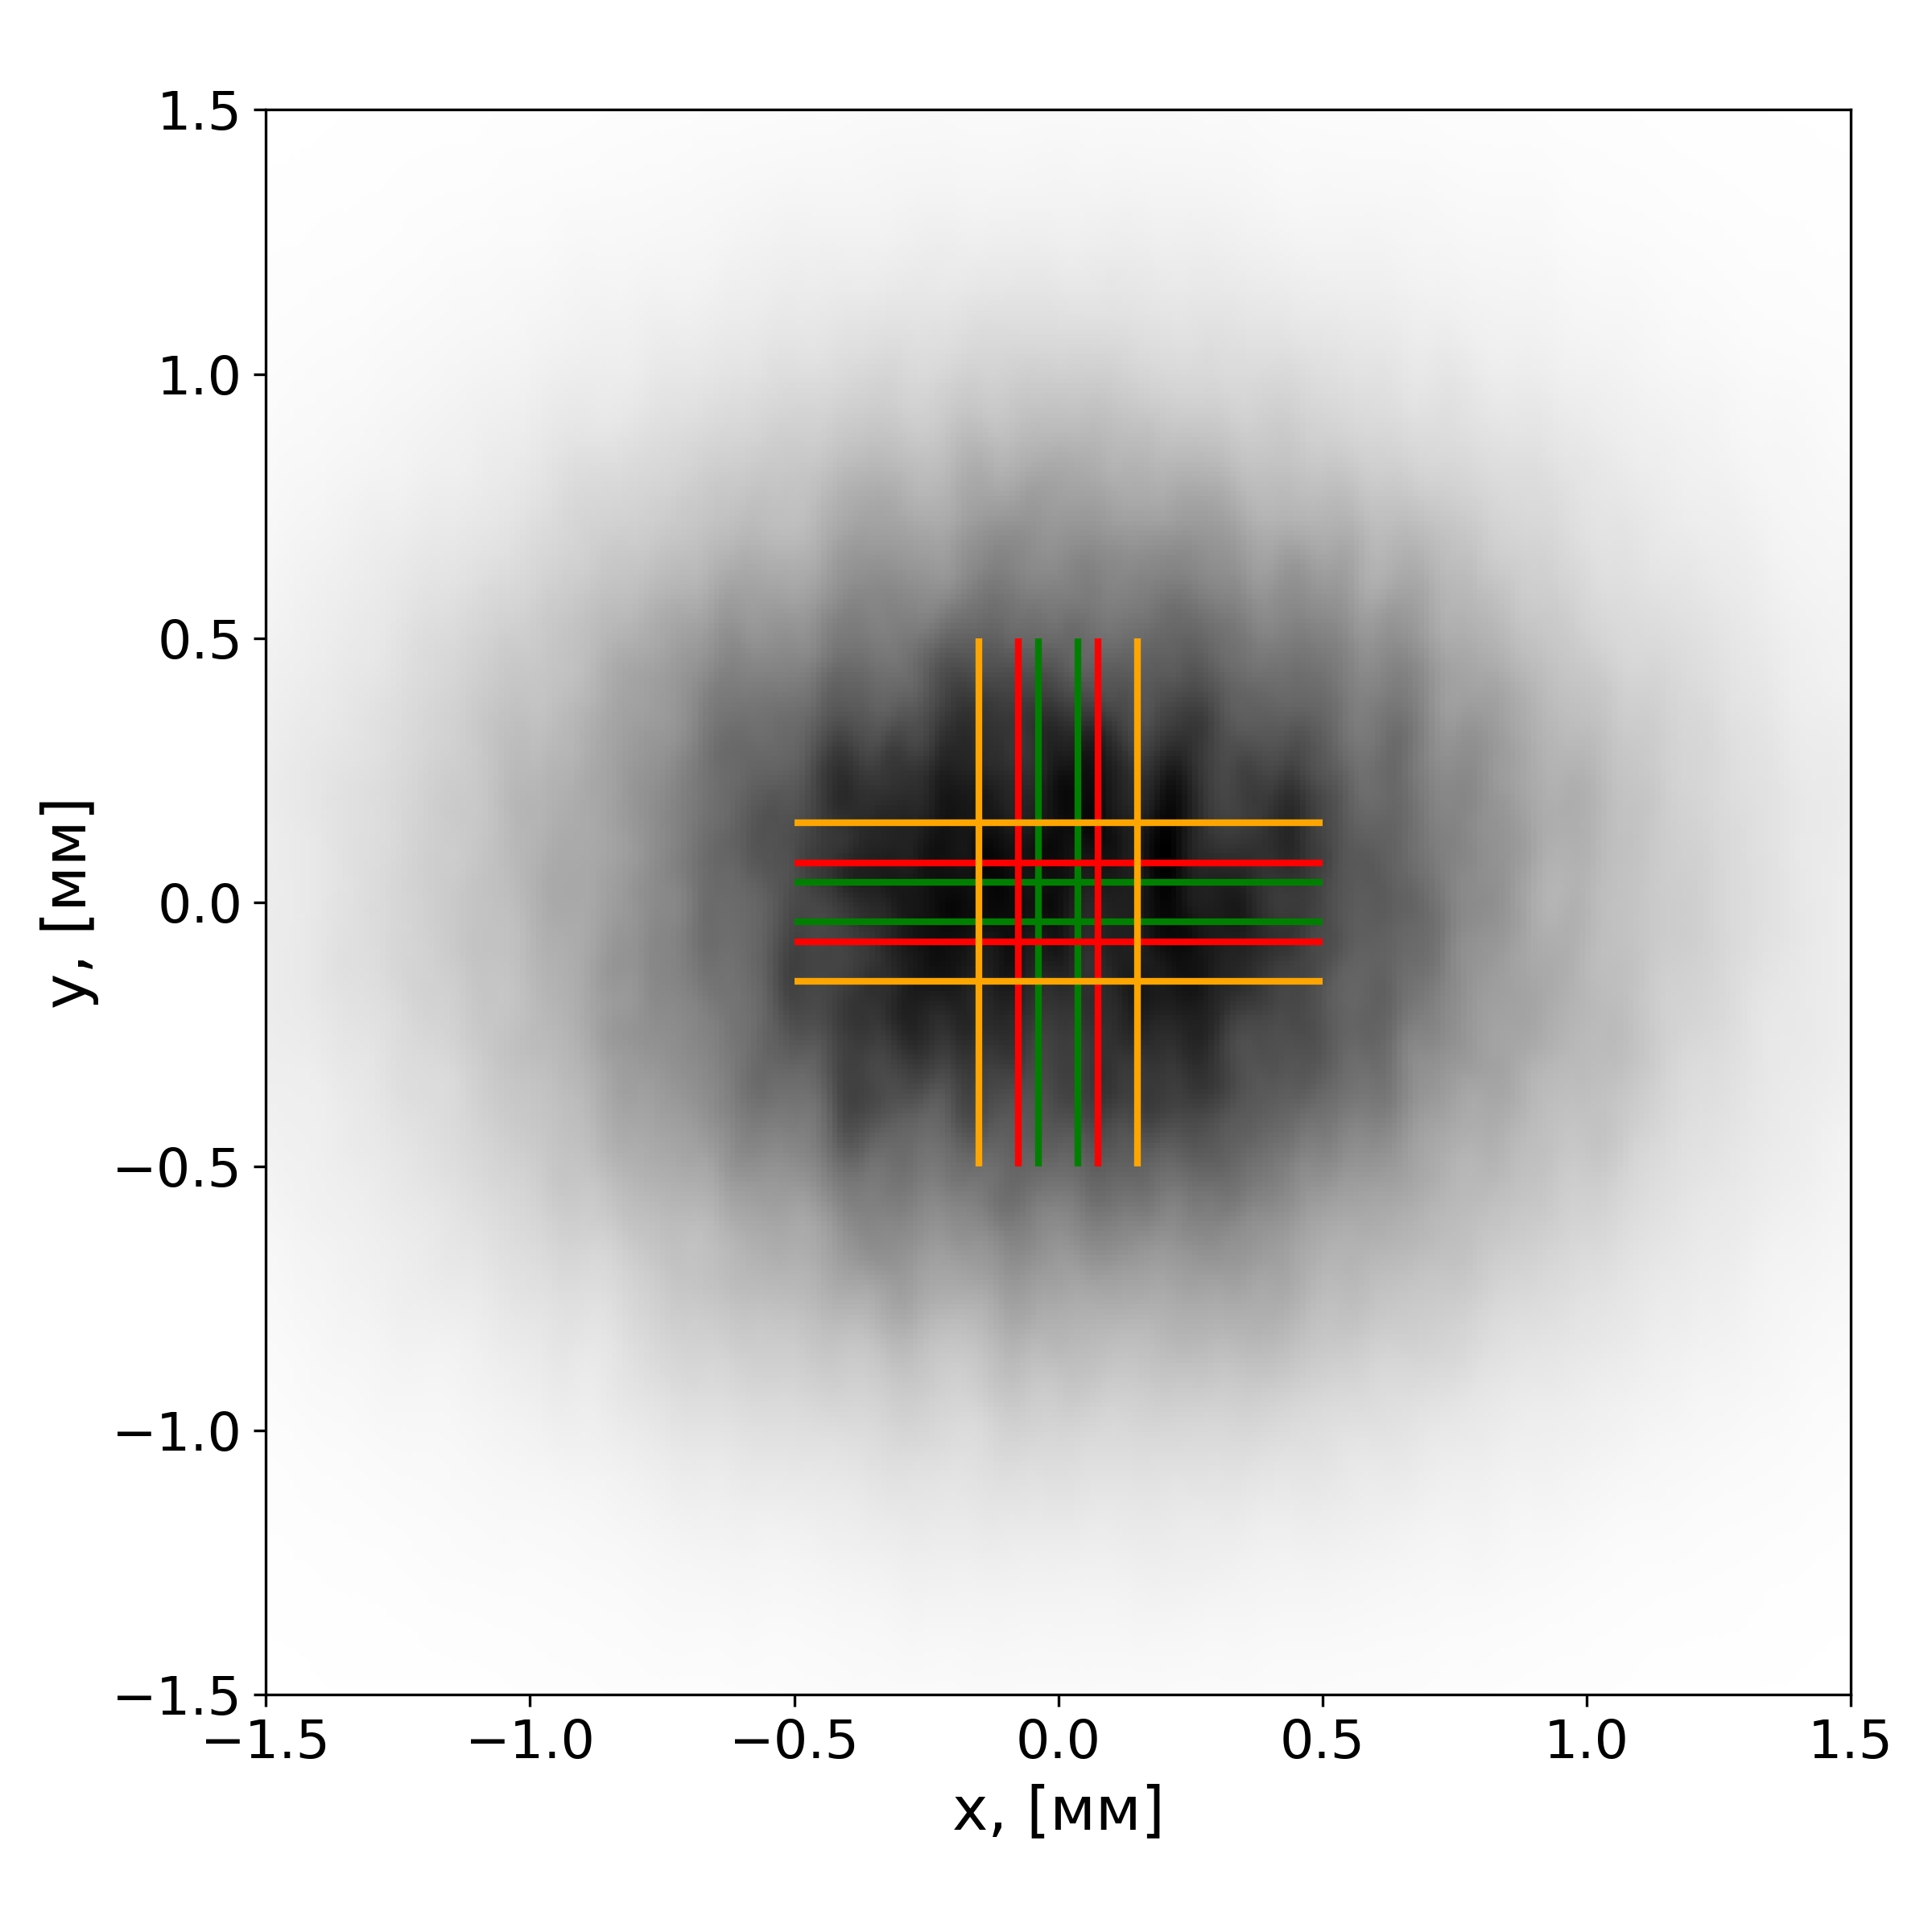
\includegraphics[width=1\linewidth]{field_before_slit.png}
		\caption{\rr{убрать вертикальные полоски}}
		\label{fig:y_field_before_slit}
	\end{minipage}
	\begin{minipage}{0.33\textwidth}
		\centering
		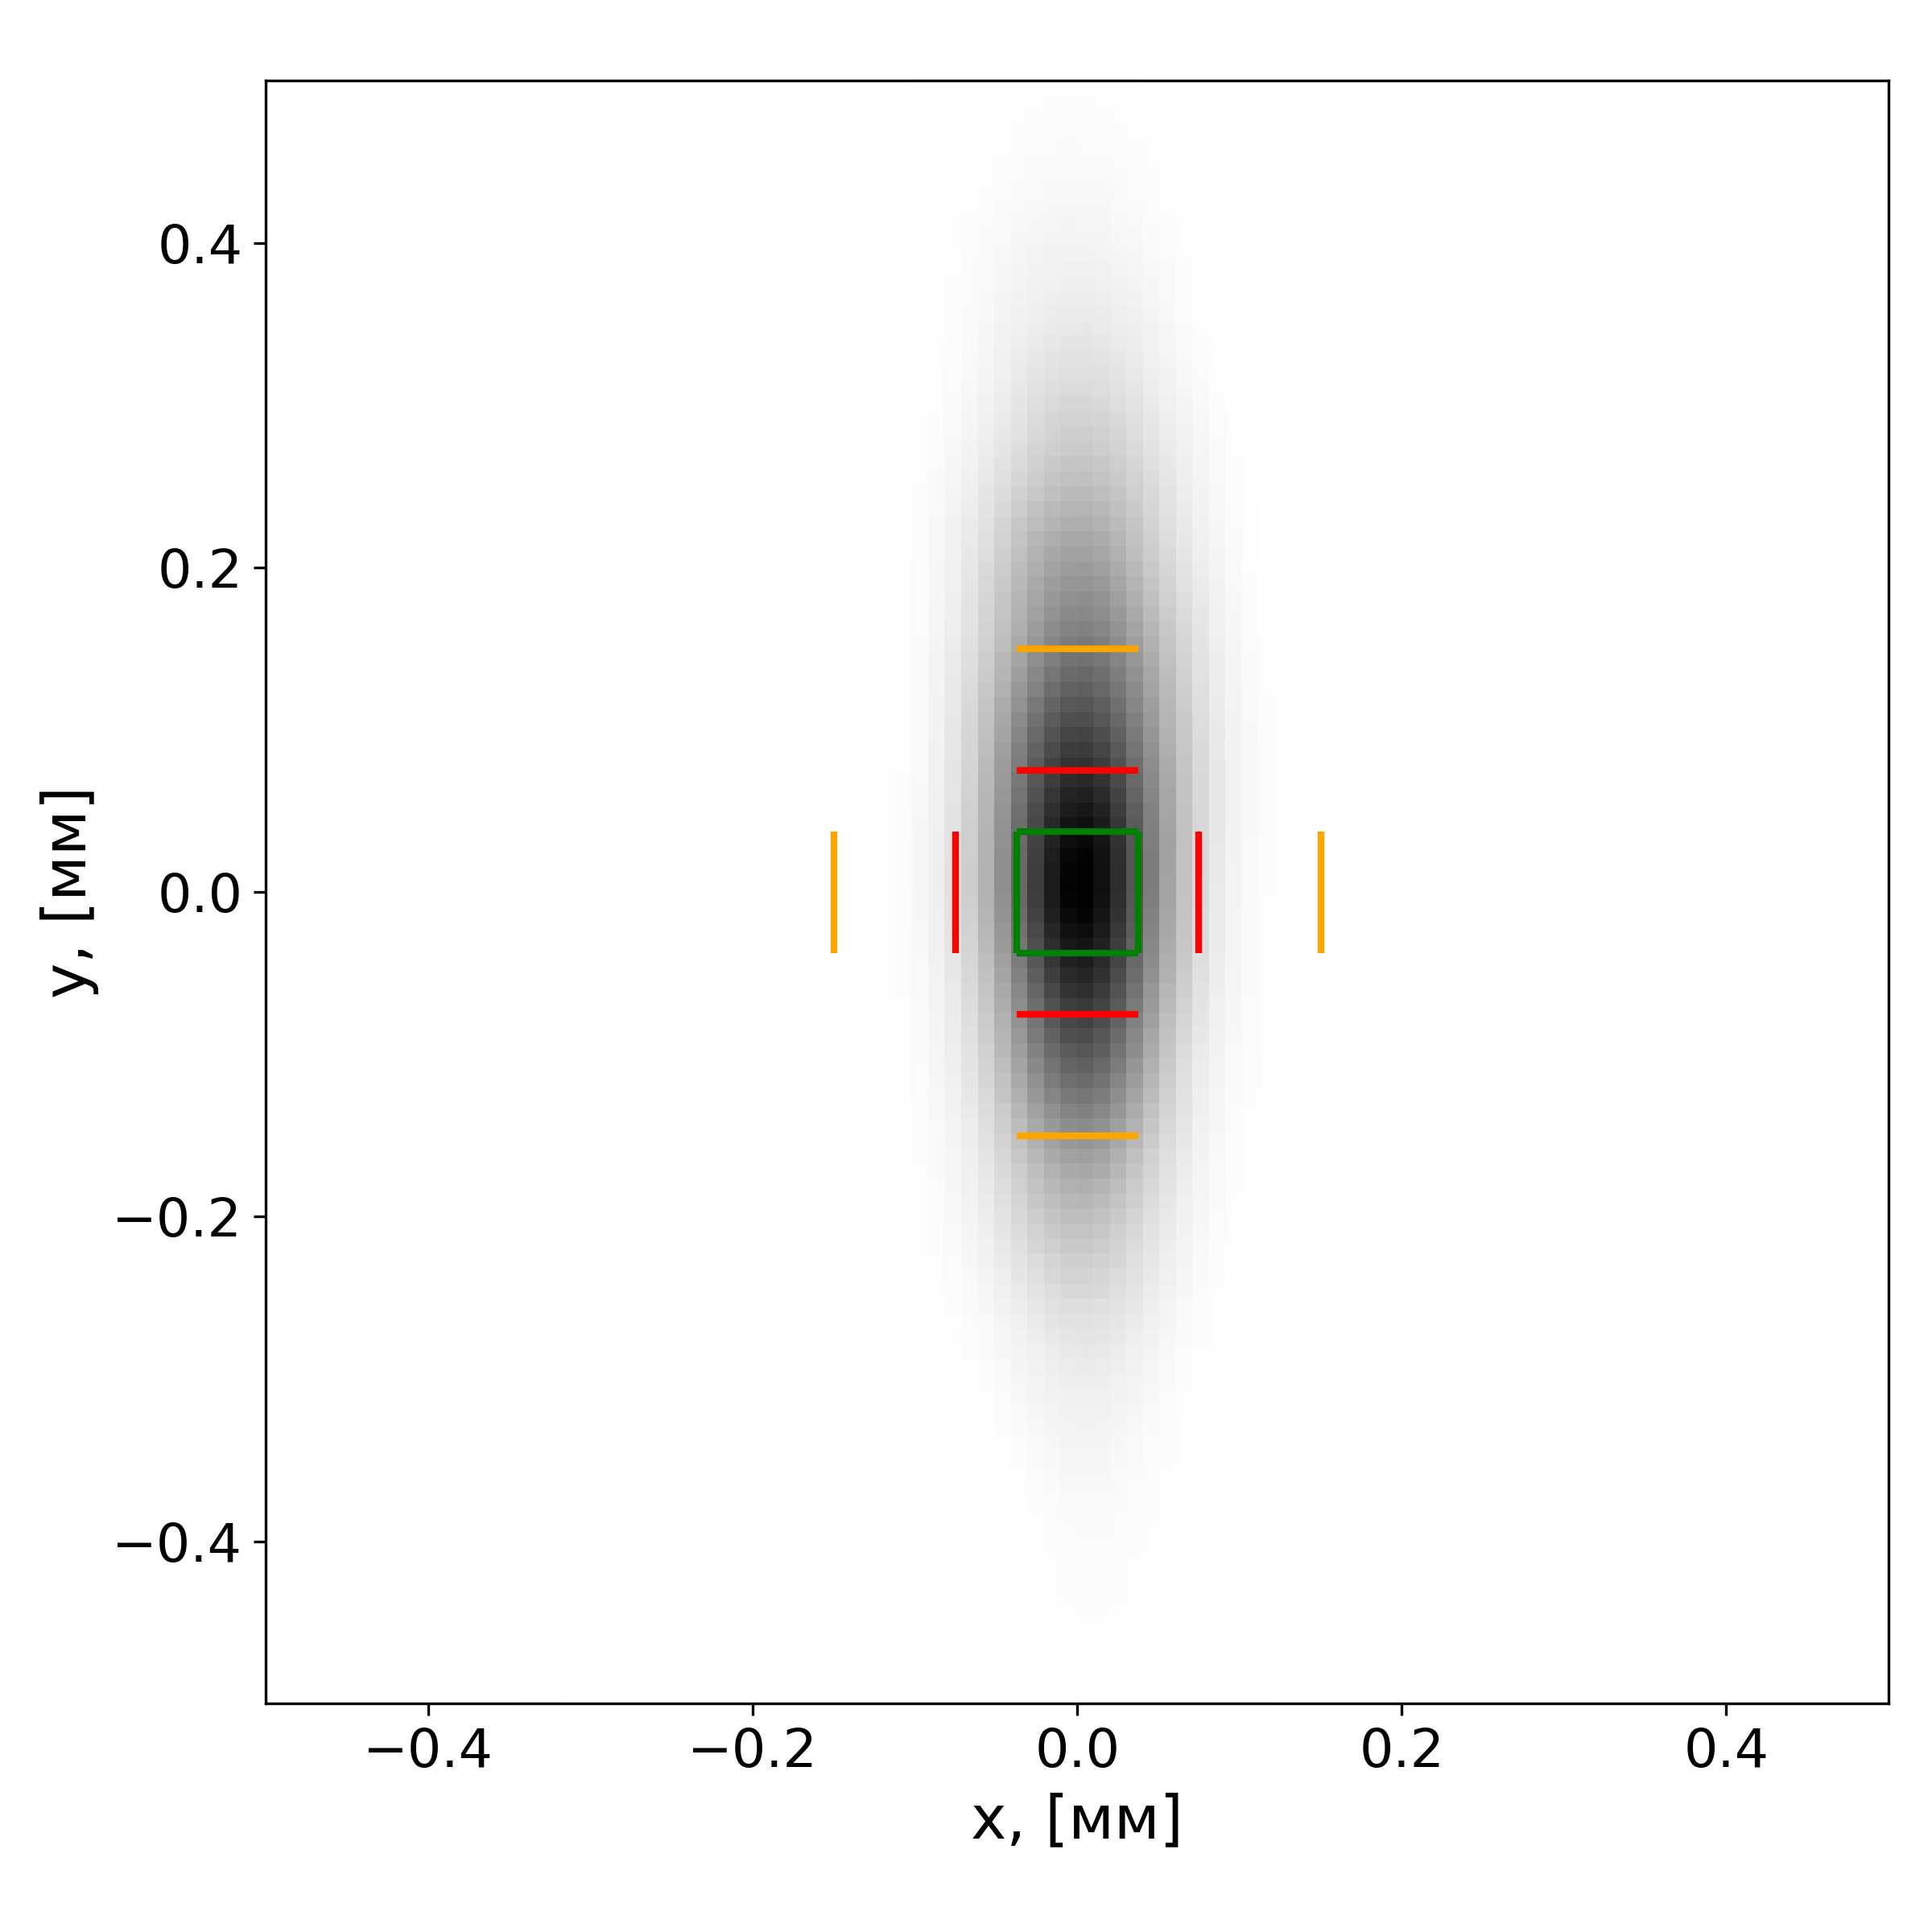
\includegraphics[width=1\linewidth]{corr_before_slit.png}
		\caption{\rr{убрать вертикальные полоски}}
		\label{fig:y_corr_before_slit}
	\end{minipage}\hfill
\end{figure}

\begin{figure}[H]
	\centering
	\begin{minipage}{0.33\textwidth}
		\centering
		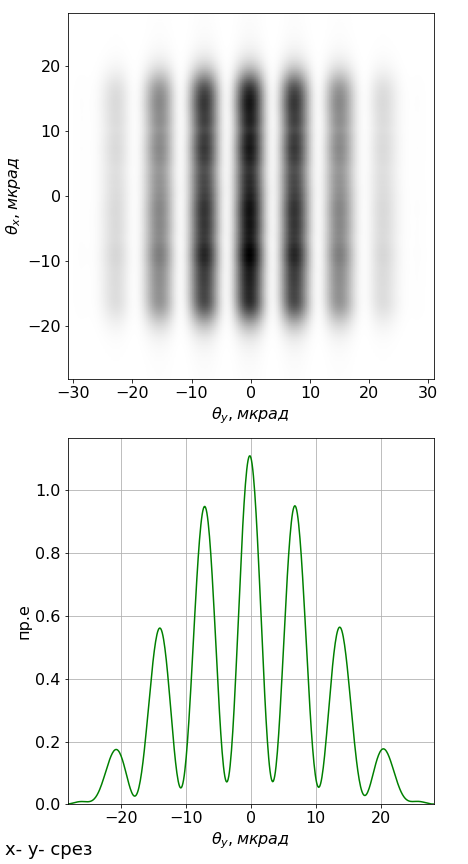
\includegraphics[width=1\linewidth]{y_slits_width_3e-05_separation_7.5e-05_.png}
		\caption{$75$ мкм}
		\label{fig:y_slits_75}
	\end{minipage}
	\begin{minipage}{0.33\textwidth}
		\centering
		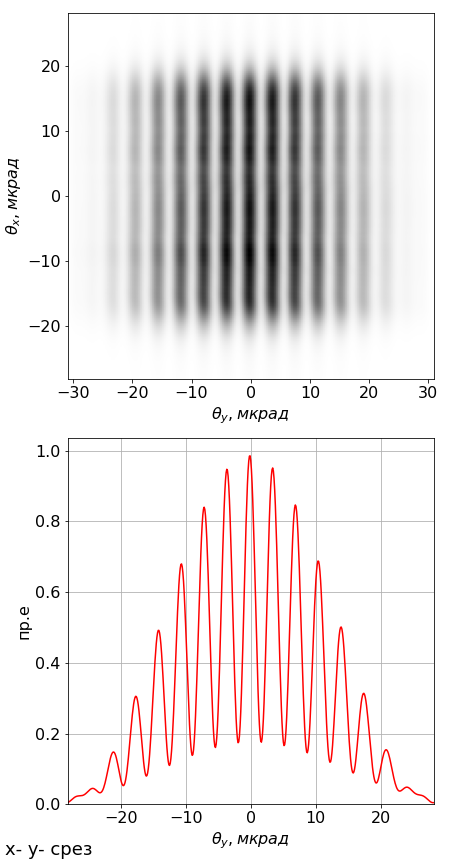
\includegraphics[width=1\linewidth]{y_slits_width_3e-05_separation_0.00015_.png}
		\caption{$150$ мкм}
		\label{fig:y_slits_150}
	\end{minipage}\hfill
	\begin{minipage}{0.33\textwidth}
		\centering
		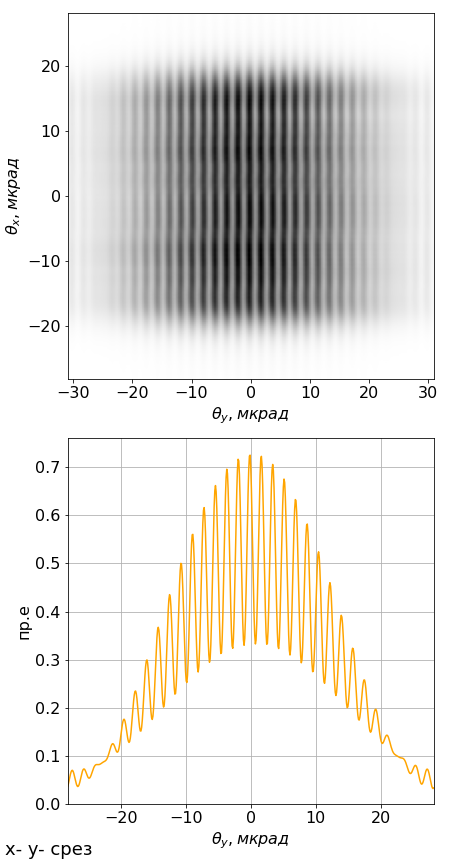
\includegraphics[width=1\linewidth]{y_slits_width_3e-05_separation_0.0003_.png}
		\caption{$300$ мкм}
		\label{fig:y_slits_300}
\end{minipage}\hfill
\end{figure}
Итак, в этом разделе показано влияние частичной когерентности излучения на формирование дифракционной картины. При частично когерентном освещении дифракционная картина «сглаживается»~\cite{goodman_statistical_2015} при уменьшении пятна когерентности или изменение характерного размера оптического элемента, в данном случае межщелевое расстояние. 

\section{Отражение от неидеального зеркала}
В этом разделе мы рассмотрим эффекты возникающие при отражении частично когерентного излучения зеркал с шероховатостями. При отражении от неидеального зеркала волновой фронт деформируется, что, при некачественной полировки поверхности, может в значительной степени влиять на размер и максимальную интенсивность излучения в фокусе, а также на когерентные свойства излучения. Ошибки по высоте $\delta h$ вносят фазовый сдвиг: 
\begin{align}
	\phi = \cfrac{4 \pi \delta h}{\lambda} \sin{(\theta_i)},
	\label{eq:roughness}
\end{align}
где $\theta_i$ -- скользящий угол на зеркало, отсчитываемый от поверхности зеркала. 

Формула~\ref{eq:roughness} даёт простой путь учёта шероховатости поверхностей при моделировании в волновом подходе, таким образом действие неидеальной поверхности учитывается как фазовый фактор, модулирующий волновой фронт. Альтернативный подход -- использование пошагового моделирования процесса отражения волнового фронта от поверхности зеркала с учётом прохождения излучения в вещество, так называемый split-step method~\cite{serkez_design_2015}. Сравнительный анализ этих двух походов приведён в работе~\cite{serkez_design_2015}, где показано совпадение оценки числа Штреля для различных значений среднеквадратического отклонения профиля зеркала, относительно идеальной поверхности. Число Штреля, описывающее относительное падение интенсивности излучения из-за наличия в оптической системе аберраций, может быть использовано для выдвижения критерия (критерий Марешаля) налагающий ограничение на среднеквадратического отклонение $h_{rms}$, а так же отклонение наклона $\mu_{rms}$~\cite{church_specification_1993}:
\begin{align}
	\cfrac{I(0)}{I_0(0)} = 1 - 8\cfrac{\mu^2_{rms}}{\theta_i} - \bigg(\cfrac{4 \pi}{\lambda} \sin{(\theta_i)} \bigg)^2 h^2_{rms} < 0,8.
	\label{eq:Marechal_criterion}
\end{align}
Здесь $I(0)$ и $I_0(0)$ интенсивность излучения на оптической оси в фокусе при отражении от неидеального зеркала и, соответственно, при отражении от идеального зеркала. 

Как видно, формула~\ref{eq:Marechal_criterion} зависит от двух параметров $h_{rms}$ и $\mu_{rms}$. Однако, обычно поверхность зеркала описывается в обратном пространстве частот -- $k$, функцией спектральной плотности $PSD(k)$ по сути являющейся Фурье преобразование профиля зеркала: 
\begin{align}
	PSD(k) =  \cfrac{1}{L} \bigg| \int_{-L/2}^{L/2} \delta h(z) \exp{(-ikz)dz}  \bigg|^2
	\label{eq:PSD_def}
\end{align}
В показано~\cite{angeisky_fractal_nodate}, профиль зеркала имеет фрактальную структуру с параметром D удовлетворяющим $1 < D < 2$, что, соответственно, даёт линейный вид $PSD$-функции в лог-лог масштабе, описываемый двумя параметрами $\alpha$ и $\beta$, при $D = (5 - \alpha)/2$. Соответственно, 
\begin{align}
	\log_{10}(PSD(k)) =  \beta \log_{10}(k) - \alpha.
\end{align}
Через $PSD$-функцию удобно определять среднеквадратичные значения ошибок по высоте и наклону через интегралы:
\begin{align}
	\mu^2_{rms} =  (2 \pi)^2 \int^{1/W}_{1/L} k^2 PSD(k) dk,
\end{align}

\begin{align}
	h^2_{rms} =  \int^{1/\lambda}_{1/W} PSD(k) dk,
\end{align}
где $W$ длина когерентности излучения на зеркале. Видно, что при некоторых значениях $W$ и параметрах оптической системы величина $\mu_{rms}$ теряет свой смысл и равна нулю. Например, для дифракционно ограниченных систем, когда $\theta_{diff} = 1.22 \lambda / D$ много больше чем видимый размер источника $\theta_{source} = \sigma_{x, y}/z_0$, где $z_0$ расстояние от источника до плоскости наблюдения. В этом случае всегда выполняется $W \sim \sqrt{2} L$, \cite{pardini_effect_2015}, и тогда применима формула $h_{rms} = \lambda / 4 \sqrt{5} \pi \theta_i$, что совпадает с аналогичными формулами у~\cite{serkez_design_2015} и~\cite{heimann_linac_2011}\footnote{$4 \pi \sqrt{5}  \approx 28$ }.

Тем не менее, $h_{rms}$ и $\mu_{rms}$ -- некоторые средние, поэтому через них сложно полно описать профиль зеркала. В идеале, при расчёте оптики необходимо знать саму $PSD$ функцию. Обращая формулу~\ref{eq:PSD_def} восстанавливается профиль зеркала~\cite{hua_using_2013},~\cite{xu_statistical_2012},~\cite{barty_predicting_2009}.
\begin{align}
	\delta h(z) = \cfrac{M}{L} F^{-1} \bigg\{\sqrt{L \cdot PSD(k)} \exp{[i \psi(k)]} \bigg\}(z),
\end{align}
где $F^{-1}{\cdot}(z)$ обратное преобразование фурье, а $M$ -- количество точек вдоль оси $z$, $\psi(k)$ -- случайно сгенерированная фаза удовлетворяющая условию $-\pi < \psi(k) <\pi$. Таким образом, зная профиль зеркала $\delta h(z)$ и используя формулу~\ref{eq:roughness}, можно провести моделирование процесса отражения волнового фронта от неидеального зеркала.

Для моделирование была выбрана та же оптическая схема что и для фокусировки с апертурой в разделе~\ref{section:focusing_system_with_aperture}. Однако, чтобы показать действие неидеального зеркала на свойства излучения, апертура была исключена из рассмотрения. На Рис.~\ref{fig:x_SERVAL_radiaiton_after_reflection_2d_3A} и~\ref{fig:y_SERVAL_radiaiton_after_reflection_2d_3A} представлены распределения излучения после отражения от неидеального фокусирующего зеркала со средним значением $h_{rms} = 0,3$ нм и после пропагации волнового фронта через $12,5$ м пустого пространства.
\begin{figure}[H]
	\centering
	\begin{minipage}{0.49\textwidth}
		\centering
		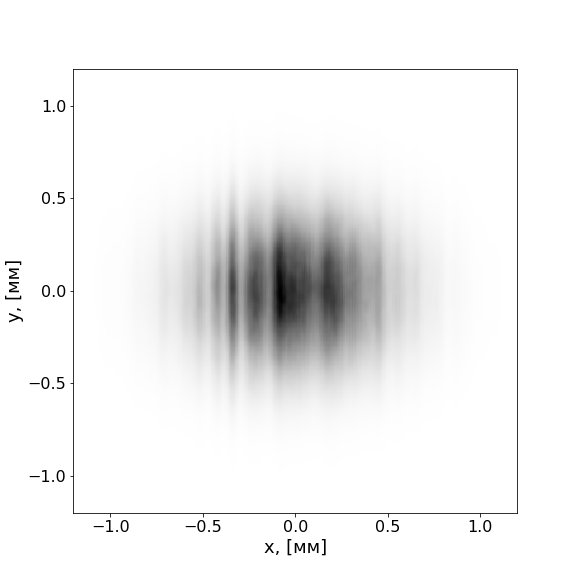
\includegraphics[width=1\linewidth]{x_SERVAL_radiaiton_after_reflection_2d_3.0_A.png}
		\caption{Распределение интенсивности излучения после отражения и $12,5$ м пустого пространства, ошибки по высоте введены по $x$}
		\label{fig:x_SERVAL_radiaiton_after_reflection_2d_3A}
	\end{minipage}
	\begin{minipage}{0.49\textwidth}
		\centering
		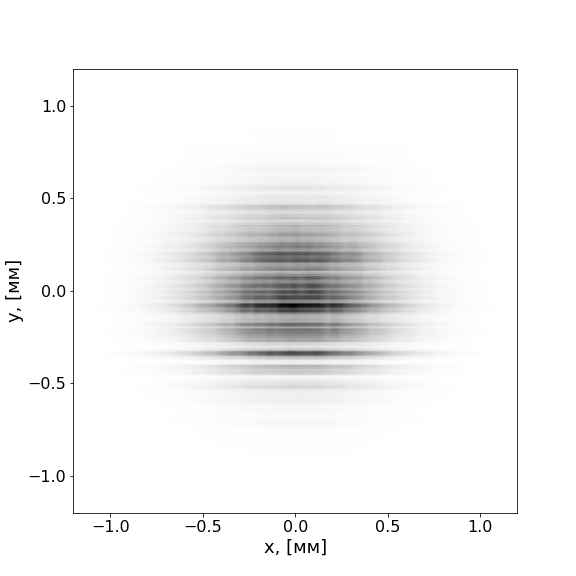
\includegraphics[width=1\linewidth]{y_SERVAL_radiaiton_after_reflection_2d_3.0_A.png}
		\caption{Распределение интенсивности излучения после отражения и $12,5$ м пустого пространства, ошибки по высоте введены по $y$}
		\label{fig:y_SERVAL_radiaiton_after_reflection_2d_3A}
	\end{minipage}\hfill
\end{figure}
\noindent Видно, для горизонтального направление модуляции волнового фронта более сглажены из-за меньшей степени когерентности в этом направлении, в отличии от вертикального направления с большей степенью когерентности.

Для сравнения того, как влияют разные профили зеркала на свойства излучения после пропагации и в фокусе на Рис.~\ref{fig:x_SERVAL_radiaiton_after_reflection},~\ref{fig:y_SERVAL_radiaiton_after_reflection},~\ref{fig:x_SERVAL_radiaiton_in_focus},~\ref{fig:y_SERVAL_radiaiton_in_focus} представлены соответствующие распределения интенсивность излучения после отражения от зеркала со среднеквадратичным отклонениями равными $0,3$ нм и $0,6$ нм. Сравнение приведено для \textit{двух ориентаций} моделируемого зеркала: ошибки введены по горизонтальному направлению  на Рис.~\ref{fig:x_SERVAL_radiaiton_after_reflection},~\ref{fig:x_SERVAL_radiaiton_in_focus}. и, соответственно, по вертикальному направлению на Рис.~\ref{fig:y_SERVAL_radiaiton_after_reflection},~\ref{fig:y_SERVAL_radiaiton_in_focus}, что соответствует вертикальному и горизонтальному ориентациям зеркал. Для всех случаев была выбрана $PSD$ функция с коэффициентом $\beta = -1,8$, нормированная на соответствующие значение среднеквадратического отклонения.

\begin{figure}[H] 
	\centering 	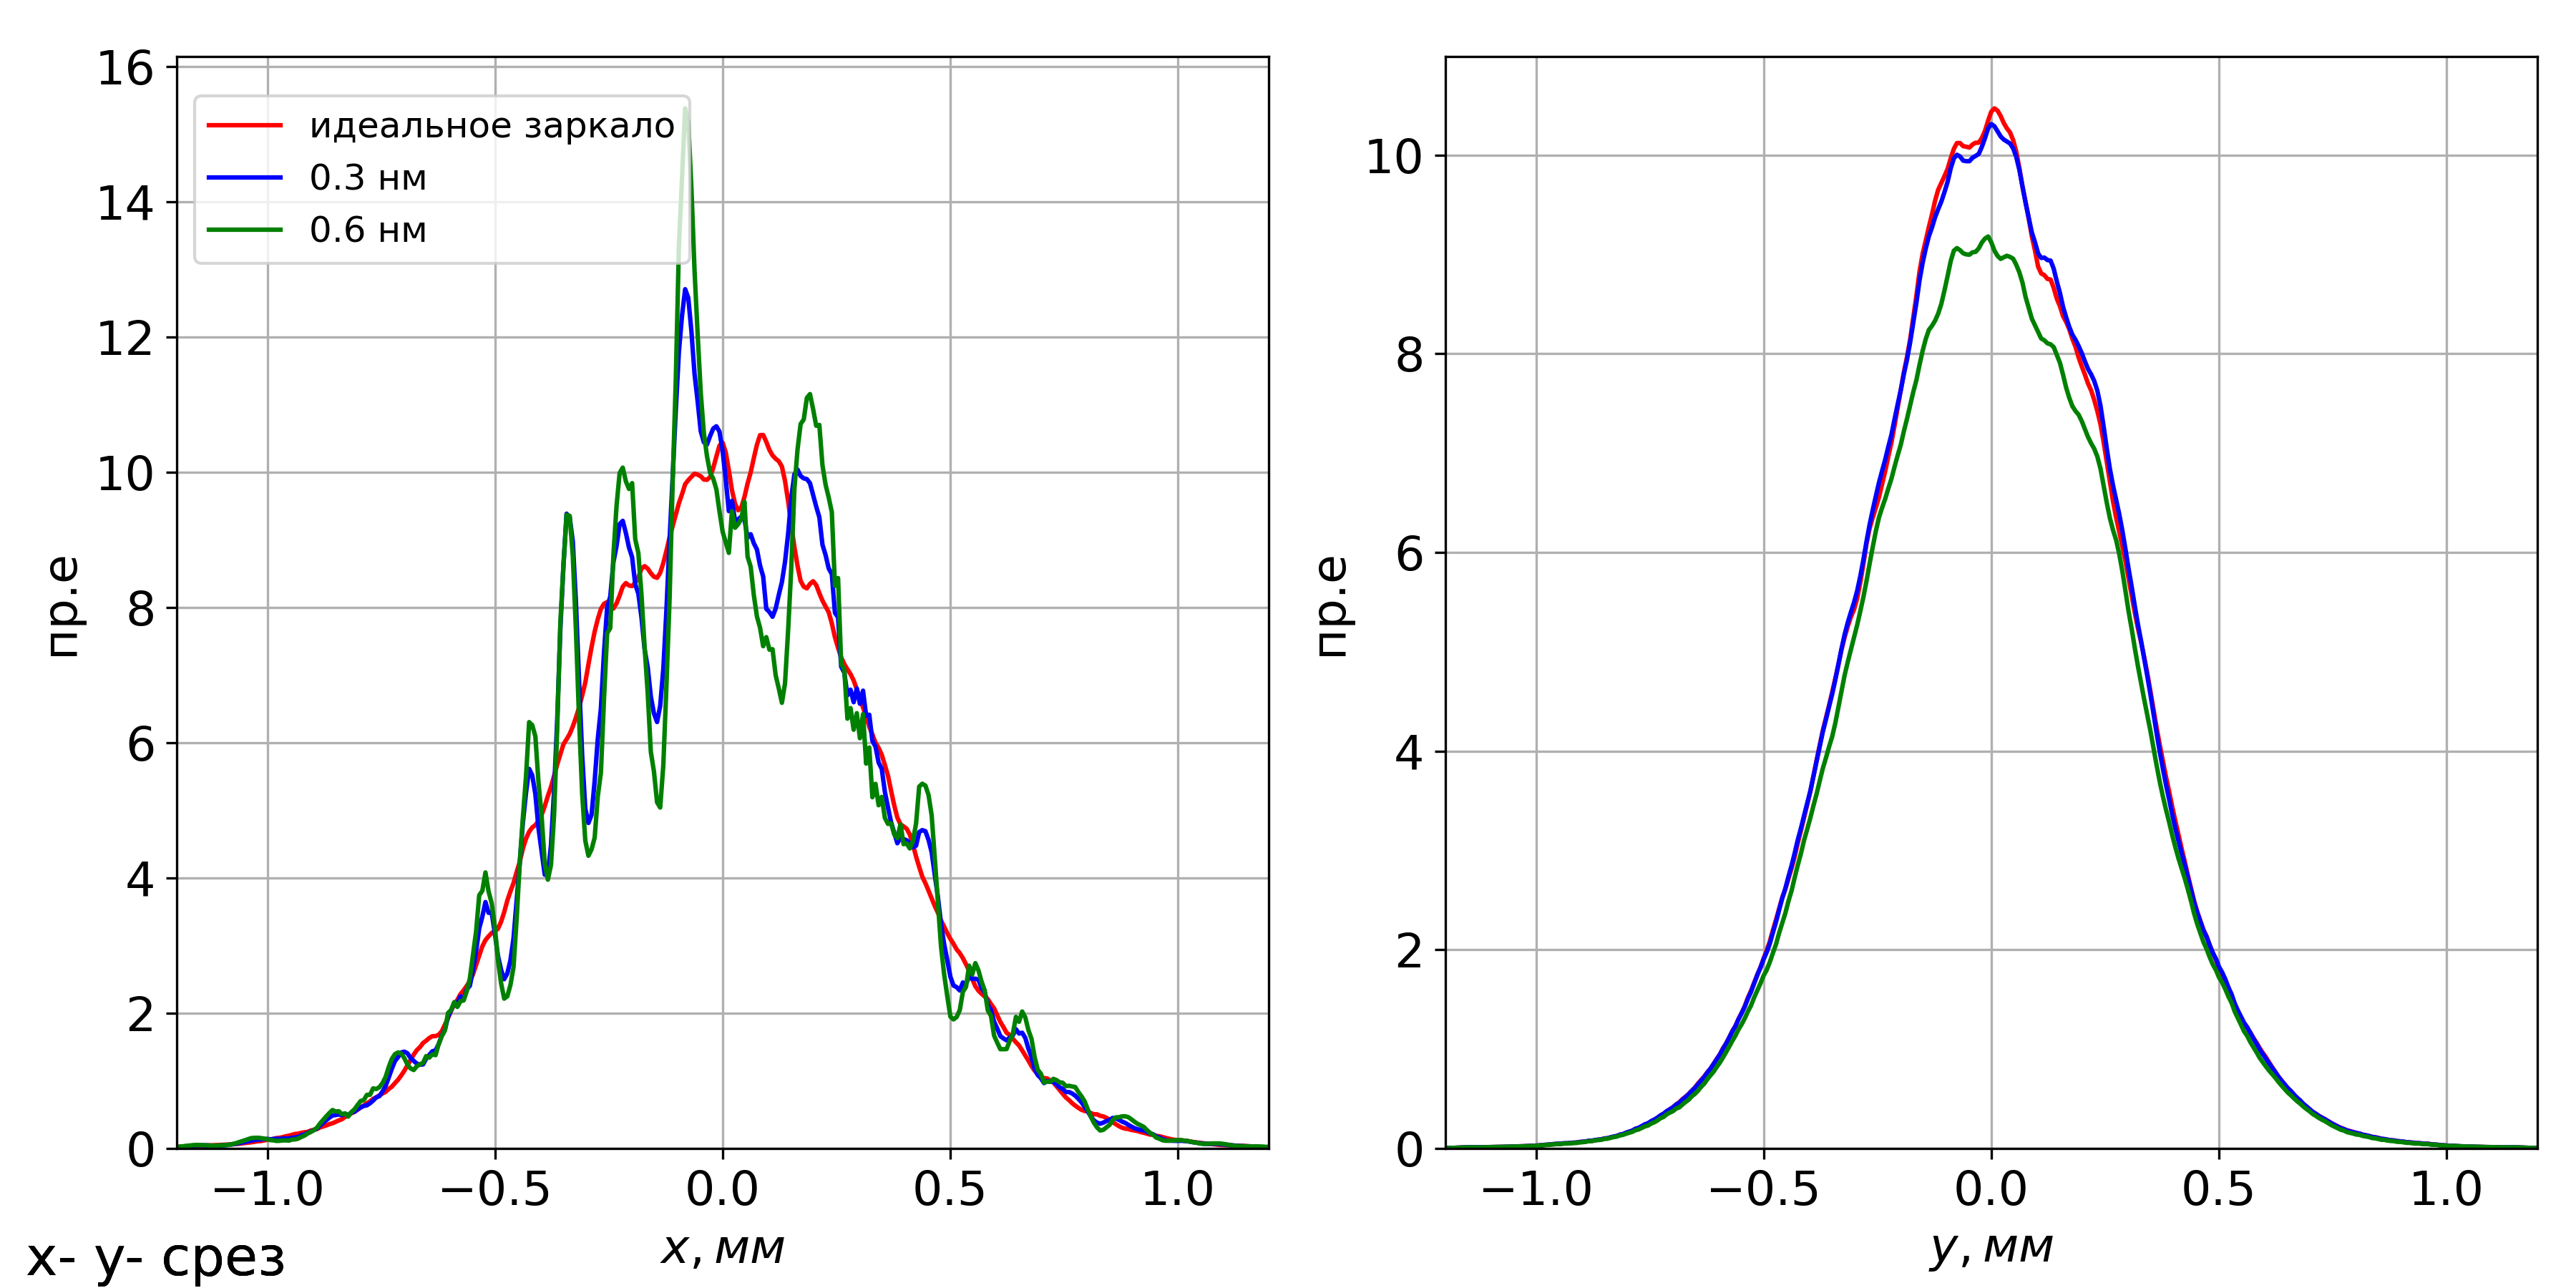
\includegraphics[width=0.99\linewidth]{x_SERVAL_radiaiton_after_reflection.png}
	\caption{Распределение интенсивности излучения после пропагции на 12.5 от зеркала, ошибки по высоте введены по горизонтальному направлению}
	\label{fig:x_SERVAL_radiaiton_after_reflection}
\end{figure}

\begin{figure}[H] 
	\centering 	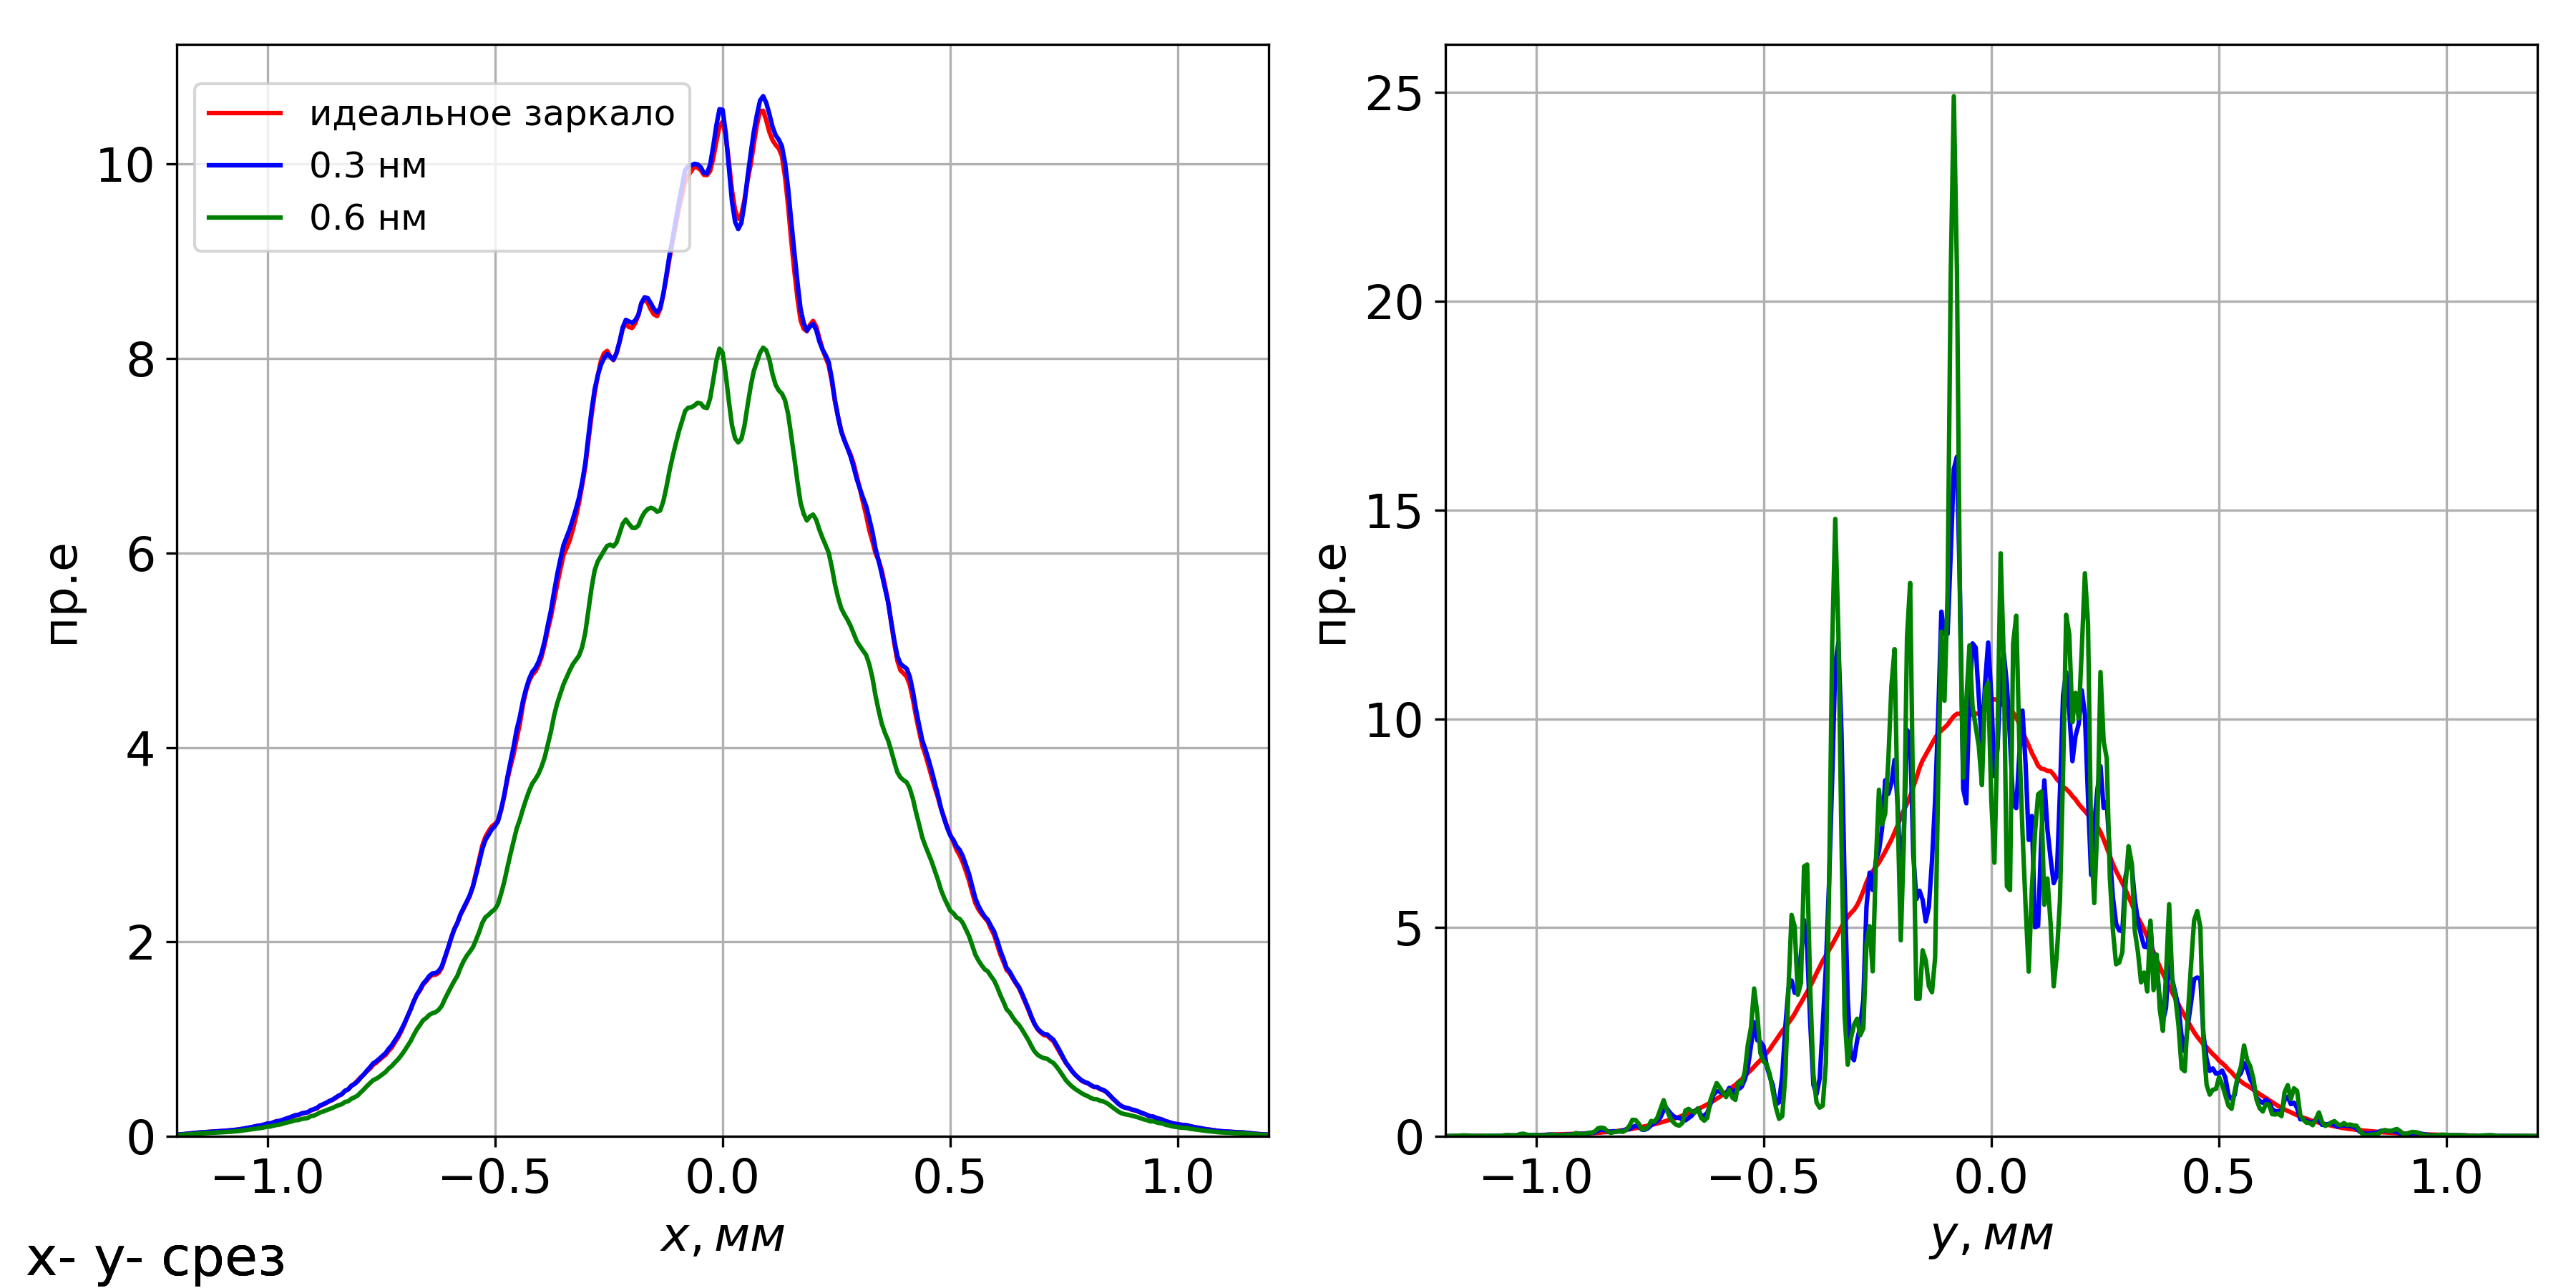
\includegraphics[width=0.99\linewidth]{y_SERVAL_radiaiton_after_reflection.png}
	\caption{Распределение интенсивности излучения после пропагции на 12.5 от зеркала, ошибки по высоте введены по вертикальному направлению}
	\label{fig:y_SERVAL_radiaiton_after_reflection}
\end{figure}
Для каждого из случаев при генерации выбиралось одинаковое начальное число (англ. seed) при генерации псевдослучайного величины, что делалось для воспроизводимости результатов. Именно поэтому модуляции волнового фронта при увеличении величины шероховатости просто повторяют свою форму, но с большей амплитудой.
\begin{figure}[H] 
	\centering 	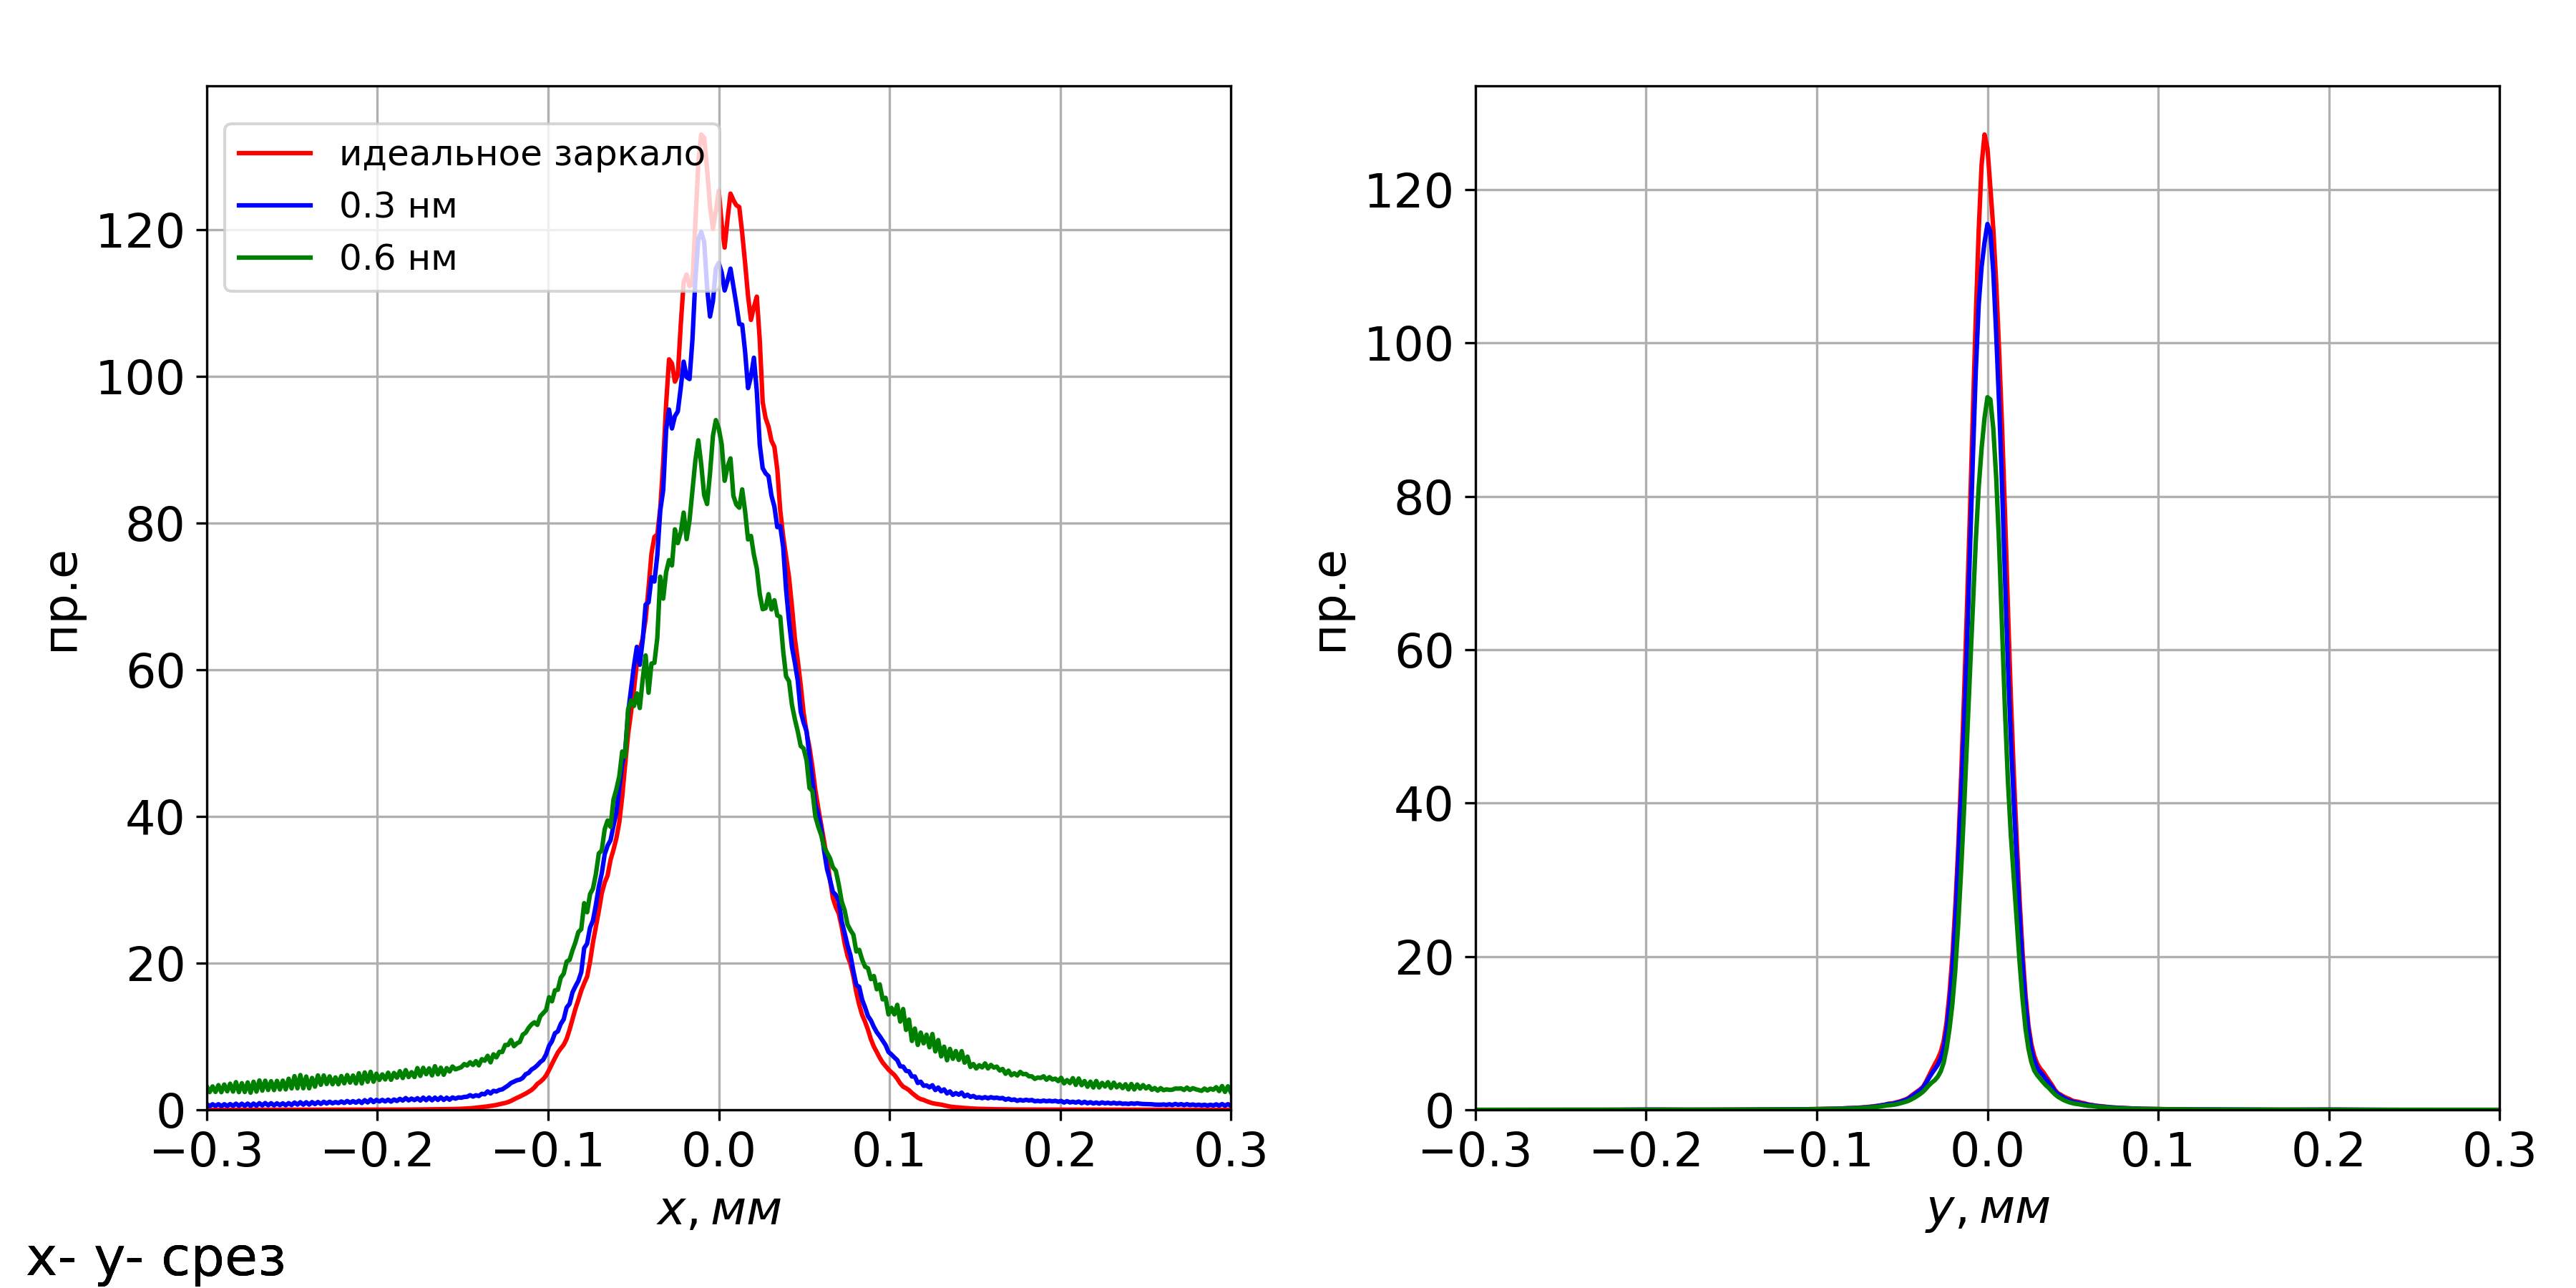
\includegraphics[width=0.99\linewidth]{x_SERVAL_radiaiton_in_focus.png}
	\caption{Распределение интенсивности излучения в фокусе, ошибки по высоте введены по горизонтальному направлению}
	\label{fig:x_SERVAL_radiaiton_in_focus}
\end{figure}

\begin{figure}[H] 
	\centering 	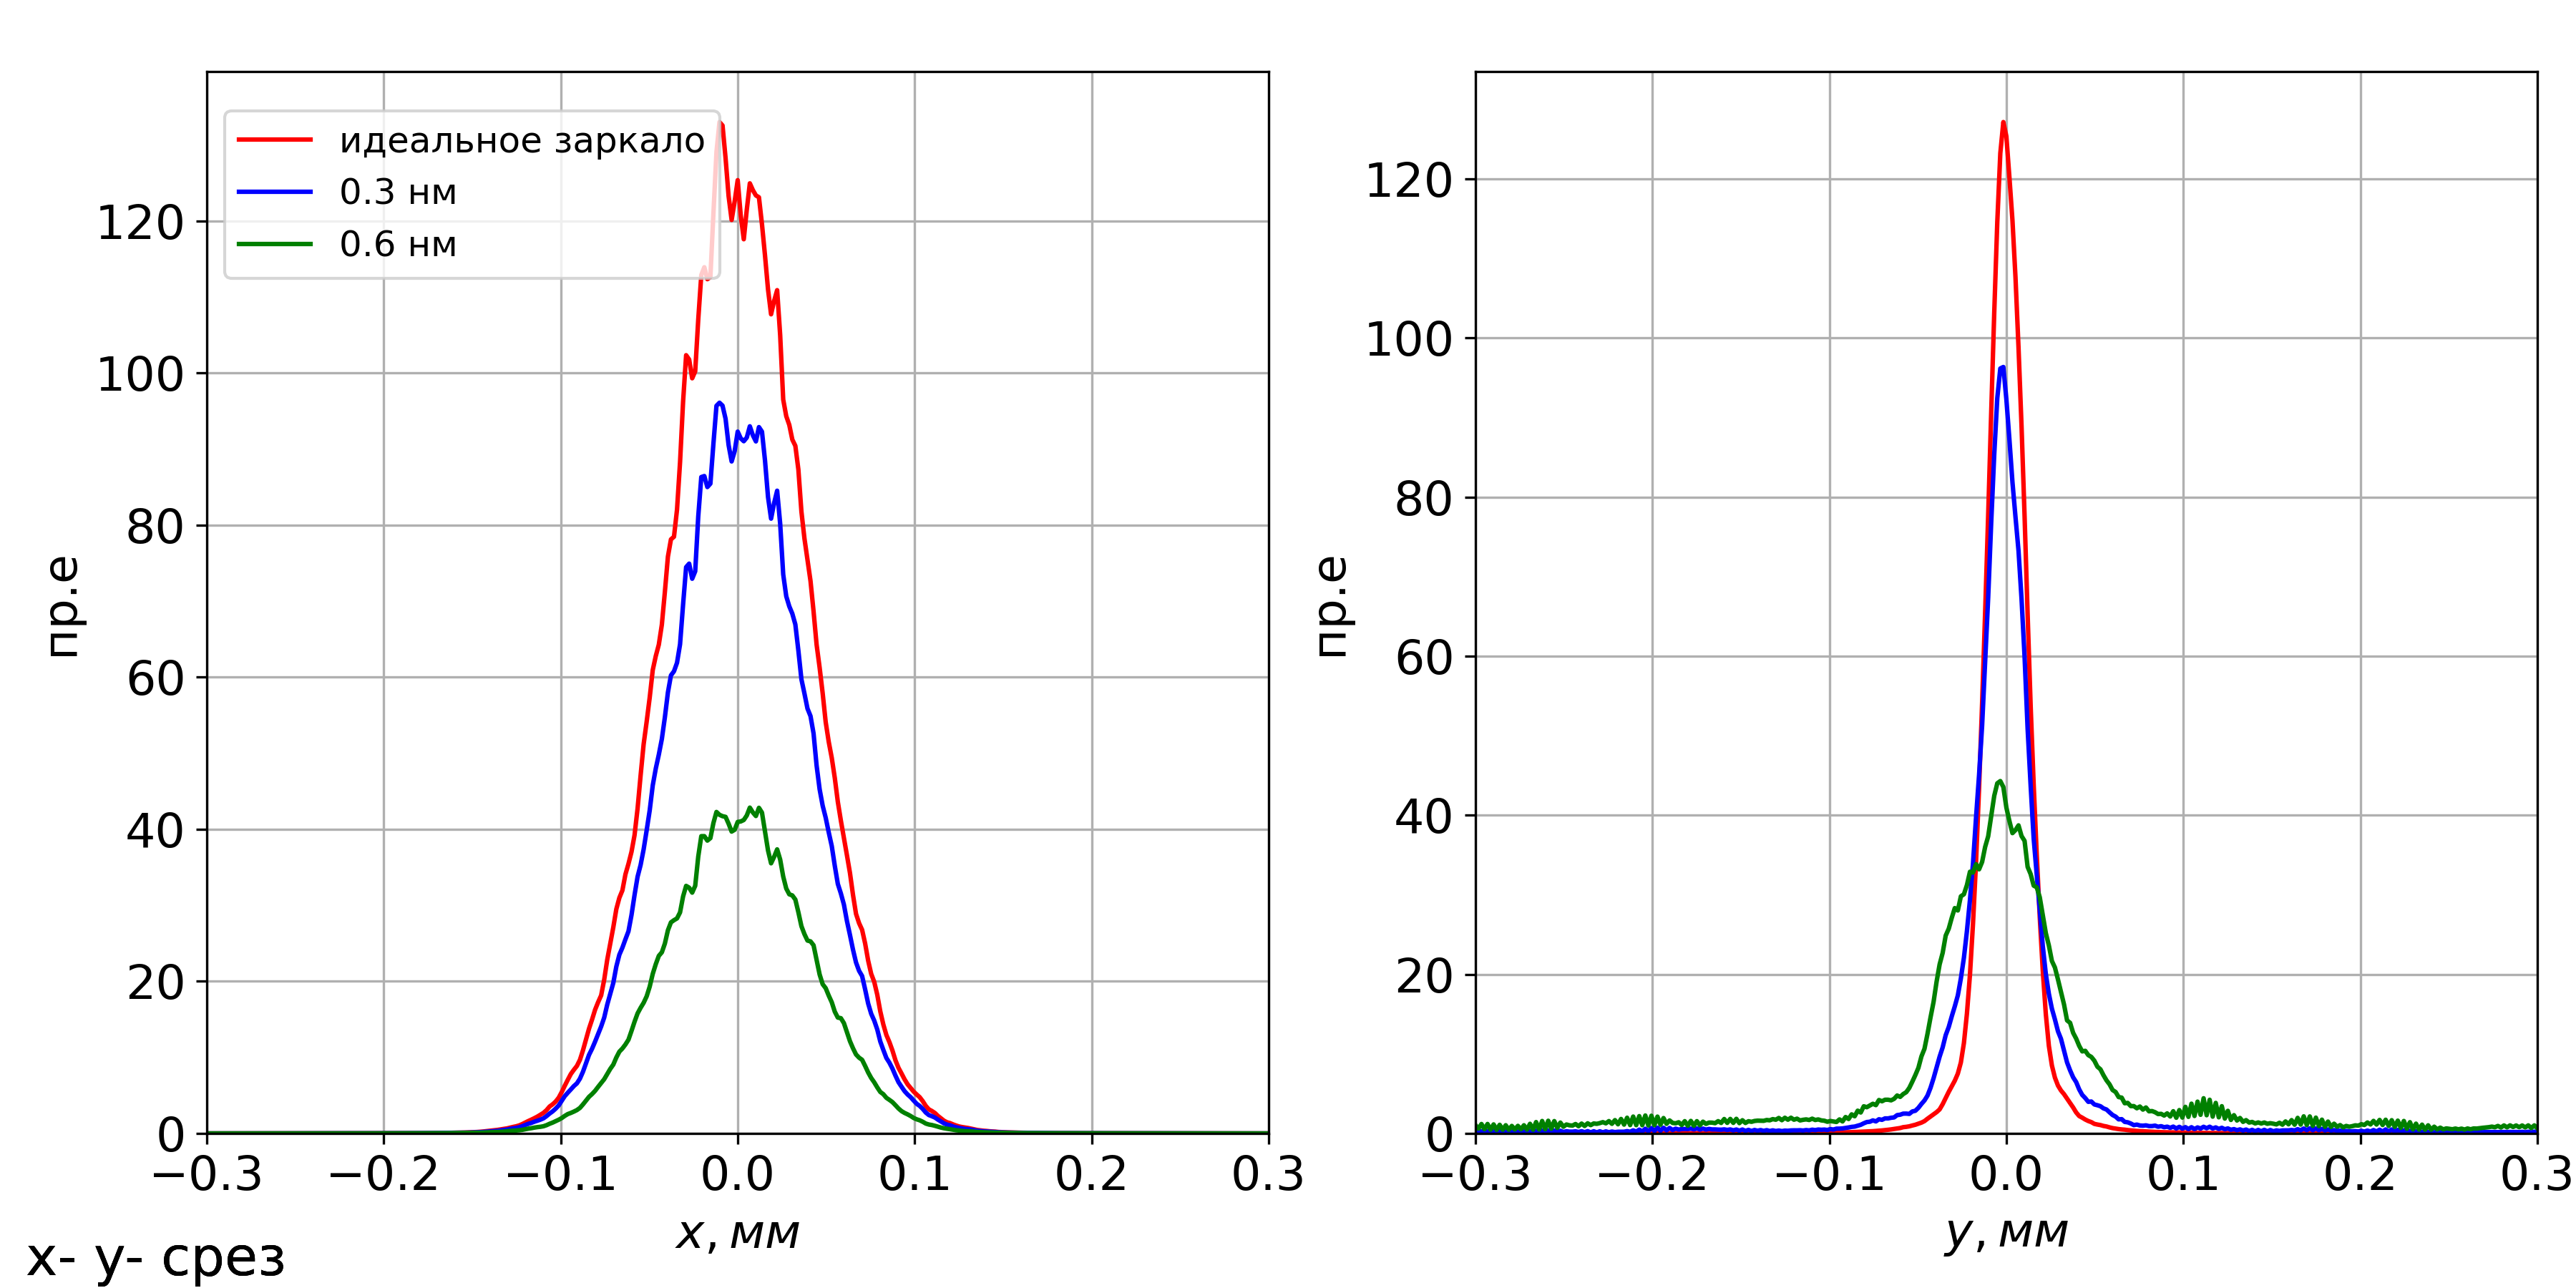
\includegraphics[width=0.99\linewidth]{y_SERVAL_radiaiton_in_focus.png}
	\caption{Распределение интенсивности излучения в фокусе, ошибки по высоте введены по вертикальному направлению}
	\label{fig:y_SERVAL_radiaiton_in_focus}
\end{figure}

Как видно на Рис.~\ref{fig:x_SERVAL_radiaiton_in_focus} и~\ref{fig:y_SERVAL_radiaiton_in_focus} шероховатости приводят к расплыванию фокусного пятна и, следственно, падению пиковой амплитуды интенсивности поля. Например, эффект увеличение размера фокусного пятна приводит к ухудшению разрешающей способности монохроматоров, основанных на дифракционных решётках, поэтому следует налагать довольно жёсткие требования на среднеквадратичную амплитуду шероховатостей рентгеновских зеркал,~\cite{strocov_high-resolution_2010},~\cite{sankari_hippie_nodate}. 

